\label{Chapter5}
 \setstretch{1.5}

%**************************************************************************************************************************************************************
%		Section I :  Introduction
%**************************************************************************************************************************************************************
\section{Introduction}
%\newcommand*{\Resize}[2]{\resizebox{#1}{!}{$#2$}}%


%Range (or distance) estimation is an important component in technologies such as electronic surveying~\cite{Jacobs_ambiguity_resolution_interferometery_1981, anderson1998surveying}, global positioning~\cite{Teunissen_GPS_LAMBDA_2006,Teunissen_GPS_1995}, and ranging cameras~\cite{time_of_flight_cam_continuous_wave_2009,Arrigo_patent_2014}. Common methods of range estimation are based upon received signal strength~\cite{Chitte_RSS_Estimation2009, HingCheung_RSSbasedRangeEstimation2012}, time of flight (or time of arrival)~\cite{XinrongLi_TOA_range_estimation2004, Lanzisera_TOA_range_estimation2011}, and phase of arrival~\cite{Fauzia_POA_range_estimation2007, Povalac_POA_rangeestimation2011}. This paper focuses on the phase of arrival method which provides the most accurate range estimates in many applications. Phase of arrival has become the technique of choice in modern high precision surveying and global positioning~\cite{Thangarajah_PDOA_rangeestimation2012, RTK_Report2003, Grejner-Brzezinska_ambguity-resolution2007, Odijk-nteger-ambiguity-resolutionPPP}. 
%
%A difficulty with phase of arrival is that only the principal component of the phase can be observed.  This limits the range that can be unambiguously estimated.  This is sometimes referred to as the problem of \emph{phase ambiguity} and it is related to what has been called the \emph{notorious wrapping problem} in the circular statistics and meteorology literature~\cite{Fisher1993}.  One approach to address this problem is to utilise signals of multiple different wavelengths and observe the phase at each.  The range can then be measured within an interval of length equal to the least common multiple of the wavelengths.  Range estimators from such observations have been studied by numerous authors.  Techniques include the beat wavelength method of Towers~et~al.~\cite{Towers_frequency_selection_interferometry_2003,Towers:04_generalised_frequency_selection}, the method of excess fractions~\cite{Falaggis_excess_fractions_2011,Falaggis_excess_fractions_2012,Falaggis_excess_fractions_2013,Falaggis_algebraic_solution_2014}, and methods based on the Chinese Remainder Theorem (CRT)~\cite{Oystein_Ore_general_chinese_Remainder_1952, Oded_Chinese_remaindering_with_errors_2000, Xia_generalised_CRT_2005, Xia2007, XWLi2008, W.Wang_closed_form_crt_2010, YangBin_range_estimation_with_CRT_2014, Xiao_multistage_crt_2014}.  Least squares/maximum likelihood and maximum a posteriori estimators of range have been studied by Teunissen~\cite{Teunissen_GPS_1995}, Hassibi and Boyd~\cite{Hassibi_GPS_1998}, and more recently by Li~et~al.~\cite{Li_distance_est_wrapped_phase} and Akhlaq~et~al.~\cite{Akhlaq_basis_construction_range_est_2015}.  A key realisation is that the least squares estimator can be efficiently computed by solving a well known integer programming problem, that of computing a \emph{closest point} in a \emph{lattice}~\cite{Agrell2002}.    Teunissen~\cite{Teunissen_GPS_1995} appears to have been the first to have realised this connection. 
We observed in previous chapters that the accuracy of the least squares range estimator is dependent upon the values of measurement wavelengths. However, the relationship between wavelengths and range estimation accuracy is nontrivial and this complicates wavelengths selection procedures. In this chapter, we develop an algorithm to automatically select wavelengths for use with the least square range estimator from~\Chap{Chapter3}~\cite{Akhlaq_basis_construction_range_est_2015}.
%In the previous chapter, we provided an upper bound on phase measurement errors for the least squares range estimator. This bound is based on the inradius of the lattice. We observed that this bound depends upon the measurement wavelengths. This naturally leads to the problem of selecting wavelengths that maximise this bound and hence the accuracy of the least squares range estimator. 
The wavelengths selection procedure is typically subject to practical constraints such as minimum and maximum wavelength (i.e. bandwidth constraints) and constraints on the maximum identifiable range. Procedures have been described for the beat wavelength~\cite{Towers_frequency_selection_interferometry_2003} and the excess fractions~\cite{Falaggis_excess_fractions_2012} methods.  Some of these methods are heuristic and require a non-negligible amount of experimentation.  Procedures for selecting wavelengths for the CRT and least squares range estimators have not yet been developed.

For the least squares estimator one possible approach for wavelength selection is to utilise the inradius of the lattice. However, the relation between the measurement wavelengths and the inradius is also nontrivial. Therefore, in this chapter, we use the relation between the wavelengths, the determinant of the lattice and its Voronoi cell to select wavelengths that maximise the accuracy of the estimator. We will notice that finding the determinant of a lattice using Corollary~\ref{cor:intlatticedim1} is simple in our case that simplifies the wavelengths selection procedure for the least squares range estimator. 

For the purpose of wavelengths selection, we devise an optimisation criterion connected with the mean square error under constraints on the minimum and maximum wavelengths and on the identifiable range.  The optimisation criterion is developed using  interesting properties of a particular class of \emph{lattices}, a structure common in algebraic and computational number theory~\cite{SPLAG,Martinet2003,cohen1993compnumtheory,McKilliam2010thesis}.  These properties lead to simple and sufficiently accurate approximations for the mean square range error in terms of the wavelengths.  The resulting constrained optimisation problem is simple enough to be minimised by a depth first search.  Monte-Carlo simulations indicate that wavelengths that minimise this criterion can result in considerably more accurate range estimates than wavelengths selected by ad hoc means.

The chapter is organised as follows. Section~\ref{ch5:sec:phase-and-range-relation}  provides an upper bound on the correct solution of the quadratic form~\ref{ch3:eq:hatz} using a well known relation between the determinant of a lattice and its Voronoi cell.  %Section~\ref{sec:lattice-theory} describes required properties from the theory of lattices~\cite{SPLAG,Martinet2003,cohen1993compnumtheory,McKilliam2010thesis}.  
The interesting properties of a particular class of lattices constructed by intersection with and projection onto a subspace are described.  These properties are used to develop simple and sufficiently accurate approximations for the mean square error of the least squares range estimator in Section~\ref{sec:appr-error-range}.  Section~\ref{sec:optim-freq-range} uses these approximations to design an optimisation criterion related to the mean square error and describes an algorithm to compute wavelengths that minimise the criterion.  The algorithm is based on depth first search and can take a long time when the number of wavelengths is not small.  For this case we describe two methods that reduce the search time at the expense of not guaranteeing that the true minimising wavelengths are found.  The results of Monte-Carlo simulations are presented in Section~\ref{sec:sim-results}.  The simulations indicate that wavelengths that minimise (or approximately minimise) the criterion can result is considerably more accurate range estimates than wavelengths selected by ad hoc means.  The simulations corroborate with existing empirical evidence suggesting that the least squares range estimator is often more accurate than other estimators~\cite{Akhlaq_basis_construction_range_est_2015,robustness_least_squares_ausctw_2016}.

%**************************************************************************************************************************************************************
%		Section II :  The estimation of phase and its relationship with range
%**************************************************************************************************************************************************************
\section{Bound on the Correctness of Wrapping Variables}\label{ch5:sec:phase-and-range-relation}

%Suppose that a transmitter sends a signal of the form
%\begin{equation}\label{eq:xtranssignal}
%s(t) = \sin (2\pi ft + 2\pi\phi)
%\end{equation}
%of known phase $\phi$ and frequency $f$ in Hertz.  The signal is assumed to propagate by line of sight to a receiver resulting in the signal 
%\begin{equation}
%y(t) = \alpha s(t - r_0/c) + \omega(t) = \alpha \sin (2\pi ft + 2\pi\theta) +  \omega(t)
%\end{equation}
%where $r_0$ is the distance (or range) in meters between receiver and transmitter, $c$ is the speed at which the signal propagates in meters per second, $\alpha$ is the amplitude of the received signal, $\omega(t)$ represents noise,
%\begin{equation}
%\theta = \phi - \dfrac{ f }{c}r_0 = \phi - \dfrac{r_0}{\lambda}
%\end{equation}
%is the phase of the received signal, and $\lambda = c/f$ is the wavelength.  Alternatively, the transmitter and receiver could be in the same location and the receiver obtains the signal after being reflected off a target.  In this case, the range of the target would be $r_0/2$. The receiver is assumed to be \emph{synchronised} by which it is meant that the phase $\phi$ and frequency $f$ are known to the receiver.  
%
%Our aim is to estimate $r_0$ from the signal $y(t)$. To do this we first calculate an estimate $\hat{\theta}$ of the principal component of the phase $\theta$.  In optical ranging applications the phase estimate might be given by an interferometer.  In sonar or radio frequency ranging applications an estimate might be obtained from samples of the signal $y(t)$ after demodulation.  Whatever the method of phase estimation, the distance $r_0$ between receiver and transmitter is related to $\hat{\theta}$ by the phase difference
%\begin{equation}
%Y = \sfracpart{\phi - \hat{\theta}} = \fracpart{ r_0/\lambda + \Phi },
%\end{equation}
%where $\Phi$ represents phase noise and $\sfracpart{x} = x - \round{x}$.  The notation $\round{x}$ denotes the closest integer to $x$ with half integers rounded up.  For all integers $k$ we have
%\begin{equation}
%Y = \fracpart{ r_0/\lambda + \Phi } = \sfracpart{(r_0 + k\lambda)/\lambda + \Phi}
%\end{equation}
%and so ranges $r_0$ and $r_0 + k \lambda$ result in the same phase difference.  For this reason the range is identifiable from the phase only if we assume $r_0$ to lie in some interval of length $\lambda$.  A natural choice is the interval $[0, \lambda)$.  This poses a problem if the range $r_0$ is larger than the wavelength $\lambda$.  
%
%A common approach to address this problem is to transmit multiple signals at multiple different frequencies and observe the phase at each. In this approach, $N$ phase estimates $\hat{\theta}_1,\ldots,\hat{\theta}_N$ and $N$ phase differences 
%%\begin{equation}\label{eq:Yndefn}
%\begin{equation}\label{eq:Yndefn}
%Y_n = \sfracpart{\phi - \hat{\theta}_n} = \fracpart{ r_0/\lambda_n + \Phi_n}, \qquad n = 1, \dots, N
%%& = \fracpart{ r_0/\lambda_n + X_n} \qquad n = 1,\dots,N 
%%& = r_0/\lambda_n + X_n - z_{0n}
%\end{equation}
%%\end{equation}
%are computed, where $\lambda_n = c/f_n$ is the wavelength of the $n$th signal and $\Phi_1,\dots,\Phi_N$ represent phase noise.  Let 
%\[
%P = \lcm(\lambda_1,\dots,\lambda_N)
%\] 
%be the least common multiple of the wavelengths.  The least common multiple is the smallest positive integer such that $P/\lambda_1, \dots, P/\lambda_N$ are all integers.  Observe that the ranges $r_0$ and $r_0 + kP$ for any integer $k$ result in the same phase differences $Y_1,\dots,Y_N$ and so $r_0$ can be uniquely identified only within an interval of length $P$.  A natural choice is the interval $[0,P)$.  The least common multiple $P$ is typically much larger than any individual wavelength and so the identifiable range can be considerably enlarged by the use of multiple wavelengths.   If $\lambda_n/\lambda_m$ is irrational for any $n$ and $m$ then the least common multiple $P$ does not exist.  In this paper we assume this is not the case and that a finite least common multiple $P$ does exist.  This is a common assumption in the literature and in practice.  %In what follows we will call the ranges $r_0$ and $r_0 + kP$ as 

In this section we utilise the concept of correct wrapping variables introduced in~\Sec{ch4:sec:phase-and-range-relation}. To motivate our wavelength selection procedure we make the assumption that the phase noise $\Phi_1,\dots,\Phi_n$ in~\ref{ch4:eq:Yndefn_vecform} are zero mean, independent and identically distributed (i.i.d.) wrapped normal random variables~\cite[p.~50]{Mardia_directional_statistics}\cite[p.~76]{McKilliam2010thesis}\cite[p.~47]{Fisher1993}.  In this case, 
\[
\Phi_n = \fracpart{\epsilon_n} \qquad n = 1, \dots, N
\]
where $\epsilon_1,\dots,\epsilon_N$ are independent and identically distributed normal random variables with zero mean and variance $\sigma^2$.  Under this assumption, the least squares range estimator from~\cite{Akhlaq_basis_construction_range_est_2015} is also the maximum likelihood estimator. Observe that
\[
Y = \fracpart{r_0/\lambda_n + \Phi_n} = \fracpart{r_0/\lambda_n + \fracpart{\epsilon_n}} = \fracpart{r_0/\lambda_n + \epsilon_n}
\]
and that the phase differences can be written in the form 
\[
Y_n =  \fracpart{ r_0/\lambda_n + \epsilon_n} =  r_0/\lambda_n + \epsilon_n + \zeta_n
\]
where the integers
\[
\zeta_n = -\round{r_0/\lambda_n + \epsilon_n} \qquad n = 1 ,\dots, N 
\]
are called \emph{wrapping variables}. The wrapping variables are related to the number of whole wavelengths that occur over the range $r_0$ between the transmitter and the receiver.  Writing in column vector form
\begin{equation}\label{ch5:eq:Yndefn_vecform}
\ybf = r_0\wbf + \epsilonbf + \zetabf
\end{equation}
where the column vectors
\[
\ybf = \left(\begin{matrix} Y_1 \\ \vdots \\ Y_N \end{matrix}\right)  \;\; 
\zetabf = \left( \begin{matrix} \zeta_1 \\ \vdots \\ \zeta_N \end{matrix}\right) \;\;
\wbf = \left( \begin{matrix} \frac{1}{\lambda_1} \\ \vdots \\ \frac{1}{\lambda_N} \end{matrix} \right) \;\; 
\epsilonbf = \left( \begin{matrix} \epsilon_1 \\ \vdots \\ \epsilon_N \end{matrix} \right) .
\]
%The $n$th element of the vector $\wbf$ is the reciprocal of the $n$th wavelength, that is, $w_n = 1/\lambda_n$.  Observe that $P$ is the smallest positive number such that the vector 
%\[
%\vbf = P\wbf = (P/\lambda_1, \dots, P/\lambda_N) \in \ints^N,
%\]
%that is, such that the elements of $\vbf = P\wbf$ are all integers.  Equivalently, $P$ is the unique positive real number such that the elements of $\vbf$ are jointly relatively prime, that is, such that 
%\[
%\gcd(v_1,\dots,v_N) = \gcd(P/\lambda_1, \dots, P/\lambda_N) = 1.
%\]



%Observe that
%\[
%Y = \fracpart{r_0/\lambda_n + \Phi_n} = \fracpart{r_0/\lambda_n + \fracpart{\epsilon_n}} = \fracpart{r_0/\lambda_n + \epsilon_n}
%\]
%and that the phase differences can be written in the form 
%\[
%Y_n =  \fracpart{ r_0/\lambda_n + \epsilon_n} =  r_0/\lambda_n + \epsilon_n + \zeta_n
%\]
%where the integers
%\[
%\zeta_n = -\round{r_0/\lambda_n + \epsilon_n} \qquad n = 1 ,\dots, N 
%\]
%are called \emph{wrapping variables}. The wrapping variables are related to the number of whole wavelengths that occur over the range $r_0$ between the transmitter and the receiver.  Writing in column vector form
%\begin{equation}\label{eq:Yndefn_vecform}
%\ybf = r_0\wbf + \epsilonbf + \zetabf
%\end{equation}
%where the column vectors
%\[
%\ybf = \left(\begin{matrix} Y_1 \\ \vdots \\ Y_N \end{matrix}\right)  \;\; 
%\zetabf = \left( \begin{matrix} \zeta_1 \\ \vdots \\ \zeta_N \end{matrix}\right) \;\;
%\wbf = \left( \begin{matrix} \frac{1}{\lambda_1} \\ \vdots \\ \frac{1}{\lambda_N} \end{matrix} \right) \;\; 
%\epsilonbf = \left( \begin{matrix} \epsilon_1 \\ \vdots \\ \epsilon_N \end{matrix} \right) .
%\]
%The $n$th element of the vector $\wbf$ is the reciprocal of the $n$th wavelength, that is, $w_n = 1/\lambda_n$.  Observe that $P$ is the smallest positive number such that the vector 
%\[
%\vbf = P\wbf = (P/\lambda_1, \dots, P/\lambda_N) \in \ints^N,
%\]
%that is, such that the elements of $\vbf = P\wbf$ are all integers.  Equivalently, $P$ is the unique positive real number such that the elements of $\vbf$ are jointly relatively prime, that is, such that 
%\[
%\gcd(v_1,\dots,v_N) = \gcd(P/\lambda_1, \dots, P/\lambda_N) = 1.
%\]
%
%Many range estimators, such as the least squares estimator and those estimators based on the CRT operate in two stages. In the first stage, an estimate $\hat{\zetabf}$ of the wrapping variables $\zetabf$ is made. Given $\hat{\zetabf}$, an estimate of the range $r_0$ is typically given by linear regression, that is, 
%\begin{equation}\label{ch5:eq:rhatlinreg}
%\hat{r}  = \frac{(\ybf - \hat{\zetabf})^\prime\wbf}{\wbf^\prime\wbf}
%\end{equation}
%where superscript $^\prime$ indicates the vector or matrix transpose.  For any integer $k$, the ranges $r_0$ and $r_0 + kP$ are equivalent and so range estimates $\hat{r}$ and $\hat{r} + kP$ for any integer $k$ are equivalent.  % To account for this, the least squares range estimator is given by~\cite[Eq.~(6)]{Akhlaq_basis_construction_range_est_2015}
%% \begin{equation}\label{hatrangeLS}
%% \hat{r}_{\text{LS}}  = \hat{r} - P \floor{\hat{r}/P}.
%% \end{equation}
%It follows that estimates $\hat{\zetabf}$ and $\hat{\zetabf} + kP\wbf$ of the wrapping variables are equivalent, because
%\[
%\frac{(\ybf - \hat{\zetabf} + kP\wbf)^\prime\wbf}{\wbf^\prime\wbf} = \hat{r} + kP.
%\]
%For this reason, the estimated wrapping variables $\hat{\zetabf}$ are to be considered error free (or correct), if $\hat{\zetabf} = \zetabf + kP\wbf$ for some integer $k$.  Because $P$ is the smallest positive integer such that $\vbf = P\wbf \in \ints^N$ this occurs if and only if $\Qbf \hat{\zetabf} = \Qbf \zetabf$ where 
%\begin{equation}\label{eq:Qproj}
%\Qbf = \Ibf - \frac{\wbf\wbf^\prime}{\wbf^\prime\wbf} = \Ibf - \frac{\vbf\vbf^\prime}{\vbf^\prime\vbf}
%\end{equation}
%is the $N \times N$ orthogonal projection matrix onto the $N-1$ dimensional subspace orthogonal to $\wbf$ and $\Ibf$ is the $N\times N$ identity matrix.  In what follows, estimates $\hat{\zetabf}$ of the wrapping variables $\zetabf$ are said to be \emph{correct} if $\Qbf \hat{\zetabf} = \Qbf \zetabf$.
It is shown in \Sec{ch3:sec:range-estim-clos-1}, that the least squares estimator $\hat{\zetabf} \in \ints^N$ of the wrapping variables minimises the quadratic form
\begin{equation}\label{eq:hatz}
\| \Qbf\ybf - \Qbf\zbf \|^2 \qquad \text{over $\zbf \in \ints^N$},
\end{equation}
%An estimate $\hat{\zetabf}$ of the wrapping variables $\zetabf$ for the least squares estimator is obtained by minimising~\cite{Akhlaq_basis_construction_range_est_2015}
%\begin{equation}\label{eq:hatz}
%F(\zetabf) = = \arg\min_{\zetabf \in \ints} \| \Qbf\ybf - \Qbf\zetabf \|^2
%\end{equation}
%The wrapping variables $\zetabf = [\zeta_1,\ldots,\zeta_n]'$ are obtained by minimising the function~\cite{Akhlaq_basis_construction_range_est_2015}
%\[
%F(\zetabf) = \| \Qbf\ybf - \Qbf\zetabf \|^2
%\]
where $\|\cdot\|$ indicates the Euclidean norm of a vector.  Given $\hat{\zetabf}$, the least square range estimator $\hat{r}$ is then given by~\ref{ch4:eq:rhatlinreg}.  It is shown in \Sec{ch3:sec:range-estim-clos-1} how the quadratic form~\ref{eq:hatz} can be minimised over $\ints^N$ by computing a closest point in a \emph{lattice}.  We will use the properties of this lattice from \Sec{sec:ch2-lattice-theory}  to develop our wavelengths selection procedure.

%\begin{figure}[t] 
%	\centering      
%		\includegraphics[scale=0.43]{figs/pdf_Comparisons.eps} 
%		\caption{Comparison of projected normal and wrapped normal distributions.}     
%		\label{fig:prognormwrappednormclose}   
%\end{figure} 
%%%%%%%%%%%%%%%%%%%%%%%%%%%%%%%%%%%%%%%%%%%%%%%%%%%%%%%%%%%%%%%%%%%%%
%\begin{figure}[t]
%  \centering 
%  \begin{tikzpicture}
%    \selectcolormodel{gray} 
%    \begin{axis}[font=\footnotesize,xmode=normal,ymode=normal,height=7cm,width=9cm,xlabel={$x$},ylabel={f(x)},ylabel style={at={(0.08,0.50)}},xlabel style={at={(0.5,0.1)}}, legend style={draw=none,fill=none,legend pos=north west,cells={anchor=west},font=\footnotesize}]
%      \addplot[solid] table {chapters/ch5/chapters/ch5/data/projectedNormalpdf1}; % 30
%      \addplot[dotted] table {chapters/ch5/chapters/ch5/data/wrappedNormalpdf1};% 0.11 (originally set to 0.08 at the start in KL distance program)
%      \node [above] at (500,80) {$\sigma^2 = 0.11$};
%      \addplot[solid] table {chapters/ch5/chapters/ch5/data/projectedNormalpdf2}; % 4.0 
%      \addplot[dotted] table {chapters/ch5/chapters/ch5/data/wrappedNormalpdf2};% 0.062 (originally set to 0.05 at the start in KL distance program )
%      \node [above] at (500,180) {$\sigma^2 = 0.06$};
%      \addplot[solid] table {chapters/ch5/chapters/ch5/data/projectedNormalpdf3}; % 0.3
%      \addplot[dotted] table {chapters/ch5/chapters/ch5/data/wrappedNormalpdf3};% 0.0076(originally set to 0.0008 at the start in KL distance program )
%      \node [above] at (540,455) {$\sigma^2 = 0.0076$};
%      \legend{Projected normal ,Wrapped normal} 
%   \end{axis}  
%  \end{tikzpicture}  
%  \caption{Comparison of projected normal and wrapped normal distributions.}\label{fig:prognormwrappednormclose}   
%\end{figure} 
%%%%%%%%%%%%%%%%%%%%%%%%%%%%%%%%%%%%%%%%%%%%%%%%%%%%%%%%%%%%%%%%%%%%%
%**************************************************************************************************************************************************************
%		Section III :  Lattice theory
%**************************************************************************************************************************************************************
%\section{Lattice theory}\label{sec:lattice-theory}
%
%Let $\mathbf{b}_1,....,\mathbf{b}_n$ be linearly independent vectors from $m$-dimensional Euclidean space $\reals^m$ with $m\geq n$.  The set of vectors
%\[
%\Lambda = \{ u_1\bbf_1 + \dots + u_n \bbf_n \mid u_1,\dots,u_n \in \ints \}
%\]
%is called an $n$-dimensional \term{lattice}.  The elements of $\Lambda$ are called \term{lattice points} or \term{lattice vectors}. 
%The vectors $\bbf_1,\dots,\bbf_n$ form a \emph{basis} for the lattice $\Lambda$.  We can equivalently write
%\[
%\Lambda=\{ \Bbf\ubf \mid \ubf \in \ints^n \}
%\]
%where $\Bbf$ is the $m\times n$ matrix with columns $\bbf_1,\dots,\bbf_n$.  %Unless otherwise stated vectors are column vectors in this paper.  
%The matrix $\Bbf$ is called a \term{basis} or \term{generator} for $\Lambda$.  The set of integers $\ints^n$ is called the \term{integer lattice} with the $n \times n$ identity matrix $\bf{I}$ as a basis.  % The basis of a lattice is not unique. If $\Ubf$ is an $n \times n$ matrix with integer elements and determinant $\det\Ubf=\pm 1$ then  $\Ubf$ is called a \term{unimodular matrix} and $\Bbf$ and $\Bbf\Ubf$ are both bases for $\Lambda$.  When $m = n$ the lattice is said to be \term{full rank}.
%When $m > n$ the lattice points lie in the $n$-dimensional subspace of $\reals^m$ spanned by $\bbf_1,\dots,\bbf_n$.  The parallelepiped formed by basis vectors $\bbf_1,\dots,\bbf_n$ is called a \term{fundamental parallelepiped} of the lattice $\Lambda$.  A fundamental parallelepiped has $n$-dimensional volume $\sqrt{\det \Bbf^\prime\Bbf }$ where $\det \Bbf^\prime\Bbf$ is the determinant of the $n\times n$ matrix $\Bbf^\prime\Bbf$.  This quantity is also called the \emph{determinant} of the lattice and is denoted by $\det\Lambda$.  
%
%Let $\Lambda$ be an $n$-dimensional lattice and let $H$ be the $n$-dimensional subspace spanned by its lattice points. The \term{dual lattice} of $\Lambda$, denoted $\Lambda^*$, contains those points from $H$ that have integer inner product with all points from $\Lambda$, that is,
%\[
%\Lambda^* = \{ \xbf  \in H \mid \xbf^\prime \ybf \in \ints \text{ for all } \ybf \in \Lambda \}.
%\]
%The determinant of a lattice and its dual are reciprocals, that is, $\det\Lambda = (\det\Lambda^*)^{-1}$~\cite[p. 10]{SPLAG}.  A lattice and its dual have interesting properties when intersected with or projected onto a subspace.
%
%\begin{proposition} \label{prop:projectedintersection}
%Let $\Lambda\subset\reals^n$ be an $n$ dimensional lattice, and let $H$ be an $n-k$ dimensional subspace of $\reals^n$.  Let $H^\perp$ be the $k$ dimensional space orthogonal to $H$ and let $p$ be the orthogonal projection onto $H$.  The set $\Lambda \cap H$ is an $n-k$ dimensional lattice if and only if $\Lambda \cap H^\perp$ is a $k$ dimensional lattice.  Moreover, if $\Lambda \cap H$ is an $n-k$ dimensional lattice then:
%\begin{enumerate}
%\item The dual of $\Lambda \cap H$ is the orthogonal projection of $\Lambda^*$ onto $H$, that is, $(\Lambda \cap H)^* = p(\Lambda^*)$.
%\item The determinants of $\Lambda$, $\Lambda \cap H$ and $\Lambda^* \cap H^{\perp}$ are related by $\det(\Lambda) \det(\Lambda^* \cap H^{\perp}) = \operatorname{det}(\Lambda \cap H)$.
%\end{enumerate}
%\end{proposition}
%\begin{proof}
%Proposition~1.3.4 and Corollary~1.3.5 of \cite{Martinet2003}.
%\end{proof}
%
%For the purpose of developing our wavelength optimisation criterion we will be particularly interested in Proposition~\ref{prop:projectedintersection} when $\Lambda$ is the integer lattice $\ints^n$ and $k = 1$.  We state this special case in the following corollary.  The corollary makes use of the fact that the interger lattice is \emph{self-dual}, that is, $\ints^n = (\ints^n)^*$.
%
%\begin{corollary} \label{cor:intlatticedim1}
%Let $\vbf\in\ints^n$ be a vector of jointly relatively prime integers, let $H$ be the $n-1$ dimensional subspace orthogonal to $\vbf$, and let
%\[
%\Qbf = \Ibf - \frac{\vbf\vbf^\prime}{\vbf^\prime\vbf} = \Ibf - \frac{\vbf\vbf^\prime}{\|\vbf\|^2}
%\]
%be the $n\times n$ orthogonal projection matrix onto $H$.  The set of vectors $\ints^n\cap H$ is an $n-1$ dimensional lattice with determinant 
%\[
%\det(\ints^n \cap H) = \|\vbf\|
%\]
%and dual lattice
%\[
%(\ints^n \cap H)^* = \{ \Qbf \zbf \mid \zbf \in \ints^n \}.
%\]
%\end{corollary}
%
%
%The (closed) \term{Voronoi cell}, denoted $\vor\Lambda$, of an $n$-dimensional lattice $\Lambda$ in $\reals^m$ is the subset of $\reals^m$ containing all points nearer or of equal distance (here with respect to the Euclidean norm) to the lattice point at the origin than to any other lattice point. If the lattice is full rank so that $n=m$ then the volume of the Voronoi cell is equal to the volume of a fundamental parallelepiped, that is, $\det\Lambda$.  Otherwise, if $m > n$ the Voronoi cell is unbounded in those directions orthogonal to the subspace spanned by the basis vectors $\bbf_1,\dots,\bbf_n$.  Specifically, if $\xbf$ is contained in this orthogonal subspace, then $\ybf \in \vor\Lambda$ if and only if $\ybf + s \xbf \in \vor\Lambda$ for all $s \in \reals$.   In this case, the intersection of the Voronoi cell with the subspace spanned by $\bbf_1,\dots,\bbf_n$ has $n$-dimensional volume equal to $\det\Lambda$.  % The Voronoi cell $\vor\Lambda$ tesselates $\reals^N$ in the sense that
%% \[
%% \reals^N = \bigcup_{\xbf \in \Lambda} (\vor\Lambda + \tbf)
%% \]
%% and $\vor\Lambda$ and a translate $\vor\Lambda + \tbf$ by a lattice point $\tbf \in \Lambda\backslash  \{\zerobf\}$ intersect at most on the boundary of $\vor\Lambda$.  The set $\Lambda \backslash  \{\zerobf\}$ denotes those lattice points from $\Lambda$ not equal to the origin $\zerobf$.  In particular, if $\interior\Lambda$ denotes the interior of the Voronoi cell, then the intersection of $\interior\Lambda$ and $\vor \Lambda + \tbf$ is empty for all $\tbf \in \Lambda \backslash  \{\zerobf\}$.  This leads to the following simple property that we will find useful.
%
%% \begin{remark}\label{remarksimpleintvor}
%% If $\tbf \in \Lambda$, $\ubf \in \vor\Lambda$, $\vbf \in \interior\Lambda$, and $\ubf = \vbf + \tbf$, then $\tbf = \zerobf$.
%% \end{remark}
%
%A \emph{short vector} in a lattice $\Lambda$ is a lattice point of minimum nonzero Euclidean length, that is, a lattice point of length
%\[
%\dmin =  \min_{\xbf \in \Lambda \backslash \{ \zerobf \} } \| \xbf \|^2.
%\]    
%The length $\dmin$ of a short vector is the smallest distance between any two lattice points.  The \emph{inradius} or \emph{packing radius} $\rho = \dmin/2$ is the length of a point on the boundary of the Voronoi cell that is closest to the origin (Figure~\ref{fig:bound_dmin}).  Equivalently, the inradius is the radius of the largest sphere that fits inside the Voronoi cell.  It is also the radius of the largest sphere that can be centered at each lattice point such that no two spheres intersect.  Such an arrangement of spheres is called a \emph{sphere packing} (Figure~\ref{fig:bound_dmin}).

Of interest to us is the probability that an $m$-variate normal random variable with i.i.d. components having zero mean and variance $\sigma^2$ lies inside the Voronoi cell.  We denote this probability by 
\begin{equation}\label{eq:probcorrectexact}
P(\Lambda, \sigma^2) = \frac{1}{\sigma^m \sqrt{(2\pi)^m}} \int_{\vor\Lambda} e^{-\|\xbf\|^2/2\sigma^2}  d\xbf.
\end{equation}
This probability can be upper bounded by the probability that an $n$-variate normal random variable lies within a sphere of $n$-volume equal to the determinant of the lattice $\det\Lambda$ using~\ref{ch2:upperBoundUsingSphere}, i.e.,
\begin{equation}\label{upperBoundUsingSphere}
P(\Lambda, \sigma^2) \leq F_n \left ( \frac{\Gamma(n/2 + 1)^{2/n} (\text{det}\Lambda)^{2/n}}{\pi \sigma^2} \right)
\end{equation}
where $F_n$ is the chi-square cumulative distribution function with $n$ degrees of freedom and $\Gamma$ is the gamma function.  This upper bound will be involved in the construction of our wavelengths optimisation criterion in Section~\ref{sec:optim-freq-range}.
The probability $P(\Lambda, \sigma^2)$ can be lower bounded by the probability that an $n$-variate normal random variable lies within a sphere of radius equal to the inradius $\rho$ of the lattice, i.e., 
\begin{equation}\label{lowerboundinradius}
P(\Lambda, \sigma^2) \geq F_n(\rho/\sigma^2).
\end{equation}
It may be possible to build an alternative wavelengths optimisation criterion using this lower bound rather than~\ref{upperBoundUsingSphere}.  However, the relationship between the wavelengths and the inradius $\rho$ is nontrivial and so we have not attempted this here. 

%Given a lattice $\Lambda$ in $\reals^m$ and a vector $\ybf \in \reals^m$, a problem of interest is to find a lattice point $\xbf \in \Lambda$ such that the squared Euclidean norm
%\[
%\| \ybf - \xbf \|^2 = \sum_{i=1}^m (y_i - x_i)^2
%\] 
%is minimised.  This is called the \term{closest lattice point problem} (or \term{closest vector problem}) and a solution is called a \term{closest lattice point} (or simply \term{closest point}) to $\ybf$ \cite{Agrell2002, MicciancioVoulgaris_deterministic_jv_2013,McKilliam_closest_point_lattice_first_kind_2014}.  The problem has found numerous applications in computer science, engineering, and statistics~\cite{Conway1983VoronoiCodes,Erex2004_lattice_decoding,Clarkson2007,McKilliam2009IndentifiabliltyAliasingPolyphase,McKilliamFrequencyEstimationByPhaseUnwrapping2009,McKilliam_mean_dir_est_sq_arc_length2010,Micciancio_lattice_based_post_quantum_crypto,McKilliam_pps_unwrapping_tsp_2014,McKilliam_fast_sparse_period_est_2015}.  The closest lattice point problem and the Voronoi cell are related in that $\xbf\in\Lambda$ is a closest lattice point to $\ybf$ if and only if $\ybf - \xbf \in \vor\Lambda$.  The closest lattice point is not necessarily unique, that is, there can be multiple lattice points that minimise $\| \ybf - \xbf \|^2$.  This occurs precisely when $\ybf - \xbf$ lies on the boundary of $\vor\Lambda$.  If $\ybf - \xbf$ is contained strictly in the interior of $\vor\Lambda$, then $\xbf \in \Lambda$ is the unique closest lattice point to $\ybf$.  In particular, if $\ybf$ itself is in the interior of $\vor\Lambda$, then the unique closest lattice point to $\ybf$ is the origin $\zerobf$.

Recall from~\ref{ch3:eq:hatz} that the least squares range estimator first computes an estimate $\hat{\zetabf} \in \ints^N$ of the wrapping variables by minimising the quadratic form $\|\Qbf\ybf - \Qbf\zbf \|^2$ with respect to $\zbf \in \ints^N$.  Recall from~\Sec{ch4:sec:phase-and-range-relation} that the $N \times N$ matrix $\Qbf$ is the orthogonal projection into the $N-1$ dimensional subspace orthogonal to the vector $\wbf$ containing the reciprocals of the wavelengths~\ref{eq:Qproj}.  Let $H$ denote this subspace.  The elements in the vector $\vbf = P\wbf$ are jointly relatively prime and so, by Corollary~\ref{cor:intlatticedim1}, the set $\Lambda = \ints^N \cap H$ is an $N-1$ dimensional lattice with determinant $\det \Lambda = \|\vbf\|$ and dual lattice $\Lambda^* = \{ \Qbf \zbf \mid \zbf \in \ints^N \}$.  We see that the problem of minimising the quadratic form~\ref{eq:hatz} is precisely that of finding a closest lattice point to $\Qbf\ybf$ in the lattice $\Lambda^*$.  

This connection between the least squares range estimator and the closest lattice point problem appears to have been first realised by~Teunissen~\cite{Teunissen_GPS_1995}.  %The notation we use here and the connection with Corollary~\ref{cor:intlatticedim1} first appeared in~\cite{Akhlaq_basis_construction_range_est_2015}.
In~\Sec{ch4:sec:phase-and-range-relation} we defined the concept of correct wrapping variables. In the next section, using the definition of correct wrapping variables, we will show that the least squares estimator $\hat{\zetabf}$ of the wrapping variables is correct when the noise $\epsilonbf$ is contained within the Voronoi cell of the lattice $\Lambda^*$.  This fact has been realised by numerous authors including Hassibi and Boyd~\cite{Hassibi_GPS_1998} who relate it to what they call the problem of~\emph{verification}.  More recently this has been utilised by Li~et~al.~\cite{Li_distance_est_wrapped_phase} and Akhlaq~et~al.~\cite{robustness_least_squares_ausctw_2016} for studying the accuracy of the least squares range estimator.  

The existing literature typically makes use of either the lower bound~\ref{lowerboundinradius} based on the inradius $\rho$ of the lattice $\Lambda^*$ or the upper bound~\ref{upperBoundUsingSphere} based on the determinant $\det\Lambda^*$.  The relationship between the wavelengths and the inradius is non trivial.  So far in the literature $\det\Lambda^*$ has been computed by first finding a basis matrix $\Bbf$ for the lattice $\Lambda^*$ and then computing the determinant directly as $\det \Lambda^* = \sqrt{\det \Bbf^\prime\Bbf }$.  The relationship between the wavelengths and the basis $\Bbf$ is nontrivial~\cite{Akhlaq_basis_construction_range_est_2015} and the determinant of the $N\times N$ matrix $\Bbf^\prime\Bbf$ is also not given by a simple expression when $N$ is not small.  For these reasons it at first appears that the relationship between the wavelengths and the determinant $\det\Lambda^*$ is non trivial.

A key realisation we make in this thesis is that $\det\Lambda^*$ is related to the wavelengths in a simple way by Corollary~\ref{cor:intlatticedim1}.  This corollary and the fact that $\det\Lambda^* = (\det\Lambda)^{-1}$ shows that $\det\Lambda^*$ takes the simple form 
\[
\det \Lambda^* = \frac{1}{\|\vbf\|} = \frac{1}{\|P\wbf\|} = \frac{1}{P \sqrt{\sum_{i = 1}^N \lambda_i^{-2}}}.
\]  
Combining this simple expression with the upper bound~\ref{upperBoundUsingSphere} will lead to a simple and sufficiently accurate approximation of the probability that the least square estimator of the unwrapping variables is correct, that is, an approximation of the probability that $\Qbf \hat{\zetabf} = \Qbf \zetabf$.  It is this simple approximation that leads to our optimisation criterion for selecting wavelengths.

%\begin{figure}[t]
%\begin{center}   
%%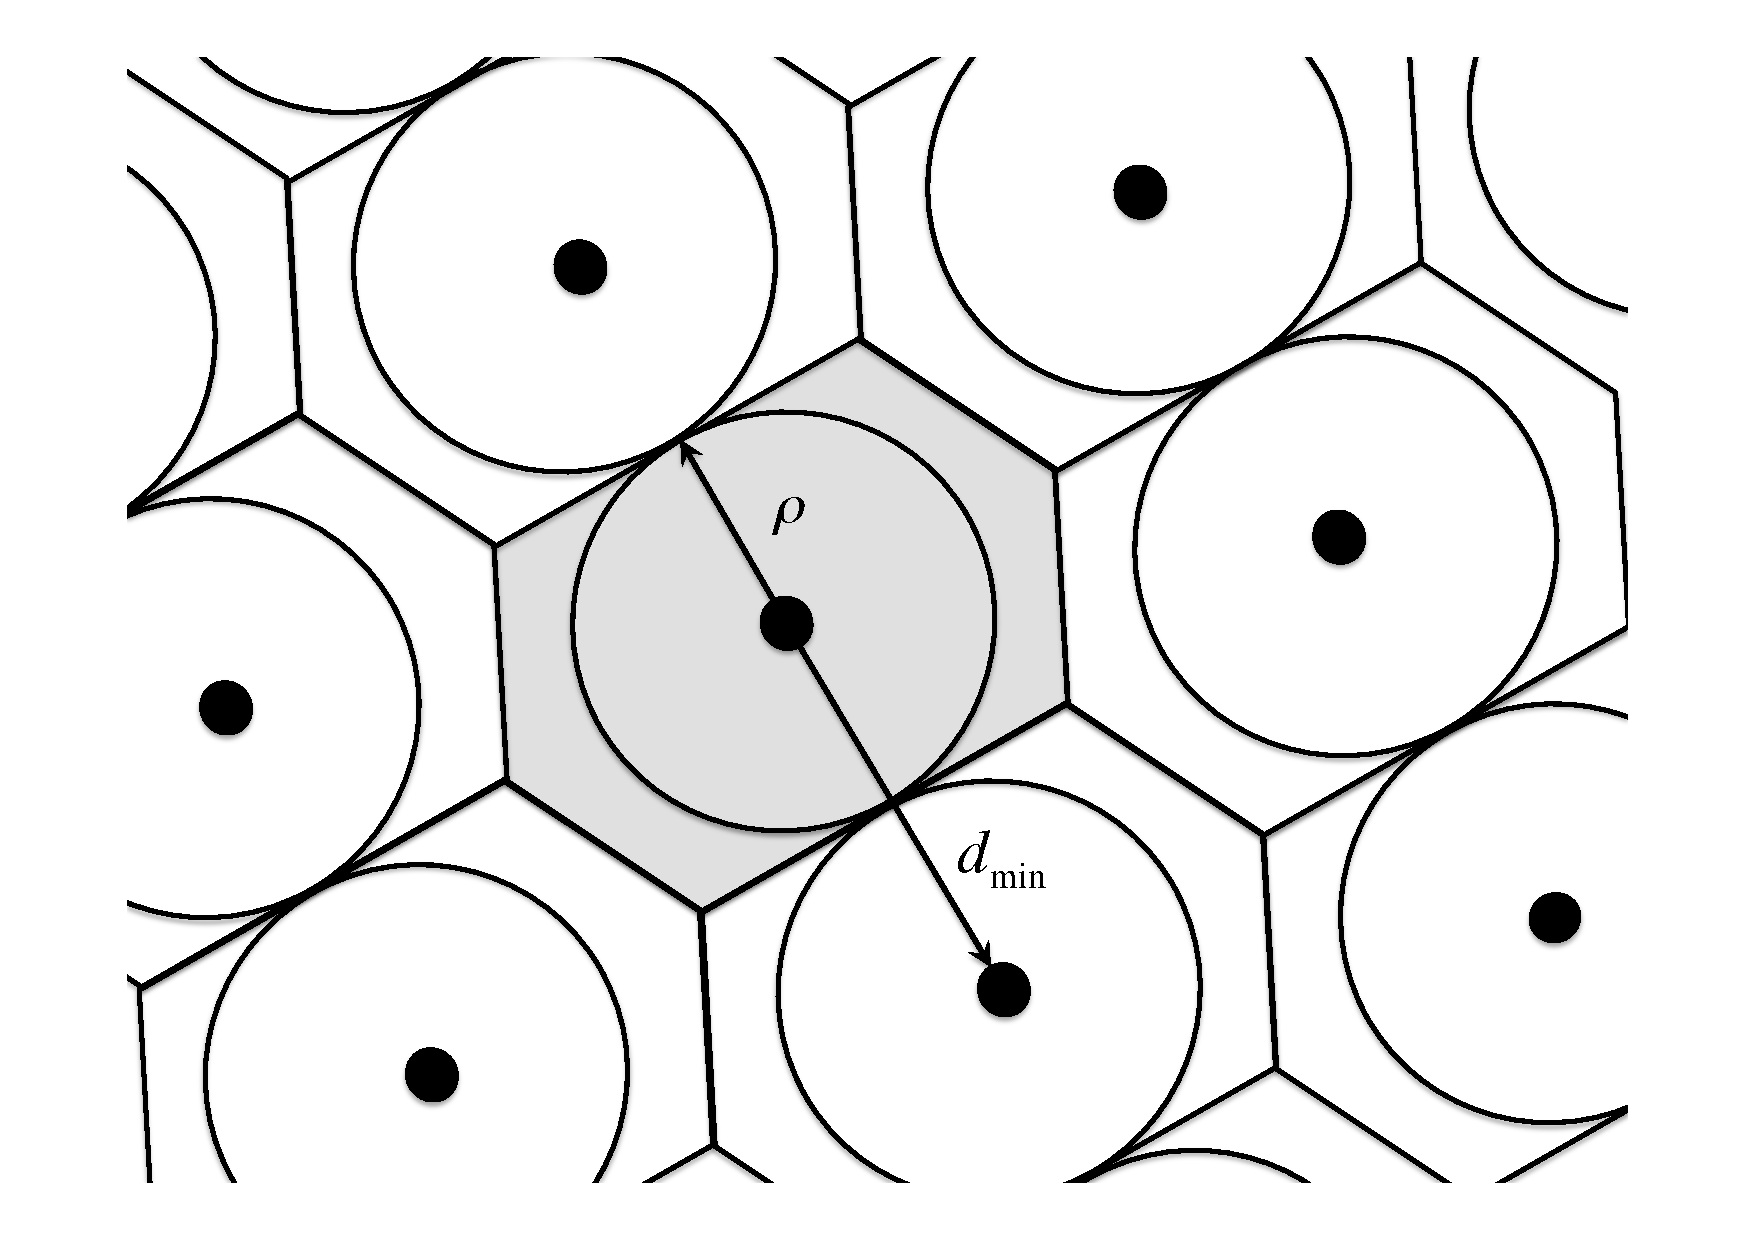
\includegraphics[scale=0.30]{figs/bound_dmin.pdf} 
%%\caption{The length of a short vector $\dmin$ and inradius $\rho = \dmin/2$ of the 2-dimensional lattice. This lattice has two short vectors. The shaded region shows the Voronoi cell of the lattice. The circles exhibit a sphere packing.}
%\includegraphics{figs/latticefigures-1.mps}
%\caption{The inradius $\rho = \dmin/2$ of the 2-dimensional lattice with basis $\bbf_1 = [3,0.72]^\prime, \bbf_2 = [0.6,3.6]^\prime$. The dots are the lattice points.  The origin $\zerobf$ is the lattice point in the center of the figure.  This lattice has two short vectors.  The shaded region shows the Voronoi cell of the lattice.  The solid circles exhibit a sphere packing.  The dashed circle has area (2-volume) equal to that of the Voronoi cell. The sphere with volume equal to the Voronoi cell is used in the upper bound~\ref{upperBoundUsingSphere}.}
%\label{fig:bound_dmin}
%\end{center}  
%\end{figure} 




%*********************************************************************************************************************************************************************************
\section{Approximating range error} \label{sec:appr-error-range}
%*********************************************************************************************************************************************************************************
In Section~\ref{sec:optim-freq-range} we will describe a procedure for selecting favourable sets of wavelengths for the least squares range estimator.  To do so, we first require approximations for the error of the range estimator in terms of the wavelengths $\lambda_1,\dots,\lambda_N$.  We consider two approximations.  The first approximates the error in the case that the least squares estimator of the wrapping variables $\hat{\zetabf}$ is correct.  The second uses~\ref{upperBoundUsingSphere} to upper bound the probability that $\hat{\zetabf}$ is correct.   

Recall from~\Sec{ch4:sec:phase-and-range-relation} that when the wrapping variables are correct $\Qbf \hat{\zetabf} = \Qbf \zetabf$ or equivalently $\zetabf = \hat{\zetabf} + k P \wbf$ for some $k \in \ints$.  In this case, the least squares estimator of the range takes the form~\ref{ch4:eq:rhatlinreg},
\[
\hat{r} = \frac{(\ybf - \hat{\zetabf})^\prime\wbf}{\wbf^\prime\wbf} = \frac{(\ybf - \zetabf + kP\wbf)^\prime\wbf}{\|\wbf\|^2}.
\]
Substituting~\ref{ch5:eq:Yndefn_vecform} for $\ybf$ we find that
\[
\hat{r} = \frac{\epsilonbf^\prime \wbf}{\|\wbf\|^2} + r_0 + kP.
\]
Recall from Section~\ref{ch4:sec:phase-and-range-relation} that range estimates $\hat{r}$ and $\hat{r} + kP$ are considered equivalent for integers $k$.  For this reason the error of the least squares range estimator corresponds with the term $\epsilonbf^\prime \wbf/\|\wbf\|^2$.  Under our assumption that $\epsilon_1,\dots,\epsilon_N$ are i.i.d. and normally distributed with zero mean and variance $\sigma^2$ this error is normally distributed with zero mean and variance
\begin{equation}\label{eq:approxwhenwrappingiscorrect}
\var \frac{\epsilonbf^\prime \wbf}{\|\wbf\|^2} = \frac{\sigma^2}{\|\wbf\|^2} = \frac{\sigma^2}{\sum_{n=1}^N \lambda_n^{-2}}.
\end{equation} 
The variance decreases as $\sum_{n=1}^N \lambda_n^{-2}$ increases.  The variance~\ref{eq:approxwhenwrappingiscorrect} serves as an approximation of the mean square error of the least squares range estimator when the estimated wrapping variables $\hat{\zetabf}$ are correct.  The simulation results in Section~\ref{sec:sim-results} suggest this approximation to be very close.

We now approximate the probability that the wrapping variables are correct, that is, we approximate the probability that $\Qbf\hat{\zetabf} = \Qbf\zetabf$.  Our approximation is based upon the upper bound~\ref{upperBoundUsingSphere}. Recall that $\hat{\zetabf}$ minimises the quadratic form $\|\Qbf \ybf - \Qbf \zbf\|^2$ over $\zbf \in \ints^N$.  It follows that $\Qbf \hat{\zetabf}$ is a closest point in the lattice $\Lambda^* = \{\Qbf \zbf \mid \zbf \in \ints^N \}$ to the point $\Qbf \ybf$.  Equivalently,
\[
\Qbf \ybf - \Qbf \hat{\zetabf} \in \vor\Lambda^*
\]
from the definition of the Voronoi cell.  Using~\ref{ch5:eq:Yndefn_vecform},
\[
\Qbf \ybf - \Qbf \hat{\zetabf} = \Qbf (r_0 \wbf + \epsilonbf + \zetabf) - \Qbf \hat{\zetabf} = \Qbf \epsilonbf - \Qbf(\hat{\zetabf} - \zetabf)
\]
and so
\[
\Qbf \epsilonbf - \Qbf(\hat{\zetabf} - \zetabf) \in \vor\Lambda^*.
\]
We see that $\Qbf(\zetabf - \hat{\zetabf})$ is a closest lattice point to the projection of the noise variables $\Qbf \epsilonbf$.  If $\Qbf \epsilonbf$ lies in the interior of the $\vor\Lambda^*$ then the unique closest lattice point is the origin $\zerobf$, that is, $\Qbf(\zetabf - \hat{\zetabf}) = \zerobf$ or equivalently $\Qbf\zetabf = \Qbf\hat{\zetabf}$.  We have found that the least square estimator $\hat{\zetabf}$ of the unwrapping variables is correct if the projection $\Qbf\epsilonbf$ of the noise variables lies within the interior of the Voronoi cell.  The estimator $\hat{\zetabf}$ can similarly be shown to be incorrect if $\Qbf\epsilonbf \notin \vor\Lambda^*$.  Because the boundary of the Voronoi cell has zero $n$-volume, it follows that the probability that unwrapping variables are correct is the same as the probability that $\Qbf\epsilonbf$ lies in $\vor\Lambda^*$

A further simplification can be made.  The $N-1$ dimensional lattice $\Lambda^*$ lies in the subspace orthogonal to $\wbf$ and so $\vor\Lambda^*$ is unbounded in the direction of $\wbf$.  Specifically, $\Qbf\epsilonbf \in \vor\Lambda^*$ if and only if $\Qbf \epsilonbf + s\wbf \in \vor\Lambda^*$ for all $s \in \reals$.  Because $\epsilonbf = \Qbf \epsilonbf + s \wbf$ for some $s$, it follows that $\Qbf \epsilonbf \in \vor\Lambda^*$ if and only if $\Qbf \epsilonbf + s\wbf = \epsilonbf \in \vor\Lambda^*$, that is,
\[
\Qbf \epsilonbf \in \vor\Lambda^* \Leftrightarrow \epsilonbf \in \vor\Lambda^*.
\]
Thus, the probability that the unwrapping variables are correct is the same as the probability that the noise $\epsilonbf$ lies in $\vor\Lambda^*$, that is, the same as the probability $P(\Lambda^*, \sigma^2)$ from~\ref{eq:probcorrectexact}.  We approximate this probability by the upper bound~\ref{upperBoundUsingSphere},
\begin{equation}\label{eq:upperboundcorrectwrapping}
P(\Lambda^*, \sigma^2) \leq F_{N-1}\left(\frac{\Gamma\big( \tfrac{N}{2} + \tfrac{1}{2} \big)^{2/(N-1)}}{\|\vbf\|^{2/(N-1)}\sigma^2 \pi}\right)
\end{equation}
where we have used the simple expression $\det\Lambda^* = \|\vbf\|^{-1}$ derived from Corollary~\ref{cor:intlatticedim1}.  This bound depends upon the wavelengths $\lambda_1,\dots,\lambda_N$ only through the term
\[
\|\vbf\|^2 = \|P\wbf\|^2 = P^2 \sum_{n=1}^N \lambda_n^{-2} = \lcm^2(\lambda_1,\dots,\lambda_N) \sum_{n=1}^N \lambda_n^{-2}.
\]
The bound increases as this term decreases.

This bound~\ref{eq:upperboundcorrectwrapping} for the probability of correct unwrapping is simpler than similar bounds in the literature that involve computing the determinant $\det\Lambda^* = \sqrt{\det \Bbf^\prime \Bbf}$ directly~\cite{Hassibi_GPS_1998,Li_distance_est_wrapped_phase}.  The simplicity of our bound is made possible by Corollary~\ref{cor:intlatticedim1} leading to the simple expression $\det\Lambda^* = \|\vbf\|^{-1}$.  This simplicity enables the wavelength selection procedure we describe in the next section.

% Substituting~\ref{eq:Yndefn} into $LS$ we obtain
% \[
% LS(r) = \sum_{n=1}^N \fracpart{\frac{r_0-r}{\lambda_n} + \Phi_n}^2.
% \] 

% Put
% \[
% z_{0n} = \round{Y_n - r_0 / \lambda_n}, \qquad n = 1,\dots,N
% \]
% and define the vector $\zbf_0 = (z_{01},\dots,z_{0N})$.  If it happens that $\hat{\zbf} = \zbf_0$ then, from~\ref{eq:leastsquaresrangehatz}, the least squares range estimator becomes
% \[
% \hat{r} = P\left( \frac{(\ybf - \zbf_0)^\prime\vbf}{\vbf^\prime\vbf} - \floor{\frac{(\ybf - \zbf_0)^\prime\vbf}{\vbf^\prime\vbf}}\right)
% \]

%*********************************************************************************************************************************************************************************
\section{Selecting wavelengths for range estimation}\label{sec:optim-freq-range}
%*********************************************************************************************************************************************************************************
In the previous section two approximations,~\ref{eq:approxwhenwrappingiscorrect} and~\ref{eq:upperboundcorrectwrapping}, related to range error were developed.  The first approximation~\ref{eq:approxwhenwrappingiscorrect} describes the variance of the range error when the wrapping variables are correct.  To decrease this variance we should choose wavelengths such that 
\[
\frac{\sigma^2}{\sum_{n=1}^N \lambda_n^{-2}}
\]
is small.  The second approximation~\ref{eq:upperboundcorrectwrapping} upper bounds the probability that the wrapping variables are correct.  To increase this bound we should choose wavelengths such that
\[
P^2 \sum_{n=1}^N \lambda_n^{-2} = \lcm^2(\lambda_1,\dots,\lambda_N) \sum_{n=1}^N \lambda_n^{-2}
\]
is small.  

\newcommand{\lambdamin}{\lambda_{\text{min}}}
\newcommand{\lambdamax}{\lambda_{\text{max}}}
\newcommand{\rmax}{r_{\text{max}}}

These are two competing objectives.  To have both small estimator variance while simultaneously allowing large probability of correct unwrapping we propose to choose wavelengths that minimise an objective function of the form
\begin{equation}\label{eq:Qobjectivefunction}
L(\lambda_1,\dots,\lambda_N) = P^2 \sum_{n=1}^N \lambda_n^{-2} + \frac{ \gamma}{\sum_{n=1}^N \lambda_n^{-2}}
\end{equation}
where $\gamma > 0$ weights the importance of the individual objectives and is free to be chosen. The weight $\gamma$ can be chosen to incorporate $\sigma^2$ if it is known.  We have found that choosing
\[
\gamma = \frac{N^2 \rmax^2}{\lambdamax^{2}\lambdamin^{2}}
\]
works well empirically.  The quantities $\rmax$, $\lambdamin$, and $\lambdamax$ will be introduced shortly.  This choice for $\gamma$ is used in the experiments performed in Section~\ref{sec:sim-results} and has the convenient property of being independent of the noise variance $\sigma^2$.  The choice is approximately the ratio of the minimum value of the two individual objectives. The motivation behind this being to approximately balance the importance given to both objectives. 

We incorporate into this optimisation problem three practical constraints.  First, we suppose that the wavelengths are all contained in an interval $[\lambdamin,\lambdamax]$.  In practice the minimum and maximum allowable wavelengths $\lambdamin$ and $\lambdamax$ might be dictated by hardware constraints, such as antennae size, or properties of the medium through which the signal propagates.  The second constraint is upon the maximum identifiable range.  We suppose that the system must be capable of unambiguously estimating range on an interval of some prespecified length $\rmax$, that is, $P \geq \rmax$.  For example $\rmax$ maybe a few meters for indoor applications, a few tens of meters for outdoor electronic surveying, and a few thousand kilometers for global positioning via satellite.  Finally, we assume that one of the wavelengths, say $\lambda_1$, is fixed and known.  We assume that $\lambda_1 = \lambdamax$ in what follows.  This constraint simplifies the optimisation problem and, since $\lambdamax$ is free to be selected, results in only minor loss of generality.  

Our optimisation problem is now to find wavelengths $\lambda_2,\dots,\lambda_{N}$ that minimise
\[
L_1(\lambda_2,\dots,\lambda_{N}) = L(\lambdamax,\lambda_2,\dots,\lambda_{N})
\]
subject to constraints
\begin{align}
&\lambdamin \leq \lambda_n \leq \lambdamax \qquad n = 2,\dots,{N} \label{eq:bandwidthcontraint} \\
&P = \lcm(\lambdamax,\lambda_2,\dots,\lambda_{N}) \geq \rmax. \label{eq:rangecontraint} 
\end{align}
These are referred to as the \emph{bandwidth constraint} and the \emph{range constraint} respectively.  The least common multiple $P = \lcm(\lambdamax,\lambda_2,\dots,\lambda_{N})$ depends upon the wavelengths in a non trivial way.  This optimisation problem is multivariate, nonlinear, and nonconvex with nonconvex constraints.  It is not immediately obvious how a solution is to be found.  We will show how this problem can be transformed into an equivalent problem involving $2(N-1)$ integer parameters.  This equivalent problem can be solved by a depth first search.

%First assume that the wavelengths are in decending order, that is, $\lambda_1 \geq \lambda_2 \geq \dots \geq \lambda_N$.  This assumption is without loss of generality because the objective function $L$ and the constraints are unchanged by permutation of $\lambda_1,\dots,\lambda_N$.  Under this assumption the range constraint can be refined to
% \begin{equation}
% \lambdamax \geq \lambda_{n-1} \geq \lambda_n \geq \lambda_{n+1} \geq \lambdamin \qquad n = 2,\dots,N-1. \label{eq:refinedbandwidthconstraint}
% \end{equation}
A solution of the minimisation problem is such that the wavelengths $\lambda_1 = \lambdamax$ and $\lambda_2, \dots, \lambda_{N-1}$ are rationally related, that is, $\lambda_n/\lambda_m$ is rational for all $n,m$.  Otherwise, $P = \lcm(\lambdamax,\lambda_2,\dots,\lambda_{N}) = \infty$ and $L_1$ will not be minimised. Thus, there exist positive integers $p_2,\dots,p_{N}$ and $q_2,\dots,q_{N}$ such that $\gcd(p_n,q_n) = 1$ and
\begin{equation}\label{eq:lambda-as-p-q}
\lambda_{n} = \frac{p_n}{q_n}\lambda_1 = \frac{p_n}{q_n}\lambdamax \qquad n = 2,\dots,N.
\end{equation}
%The case when $n = 1$ above asserts that $p_1 = q_1 = 1$.  %Also, because $\lambda_1 \geq \lambda_n$ we have $q_n \geq p_n$.  
Now,
\begin{equation}\label{eq:P-as-p-q} 
P = \lcm\left(\lambdamax, \frac{p_2}{q_2}\lambdamax, \dots, \frac{p_N}{q_N}\lambdamax \right) = \lambdamax Q
\end{equation}
where
\[
Q = \lcm\left(1,  \frac{p_2}{q_2}, \dots, \frac{p_N}{q_N} \right).
\]
A simpler expression for $Q$ can be obtained.  %First observe that $\lcm(d,a/b) = \lcm(d,a)$ is an integer if $d$ is an integer and $a$ and $b$ are relatively prime integers.  
Let $\ell_1,\dots,\ell_N$ satisfy
\[
\ell_1 = 1, \qquad \ell_{n} = \lcm\left( \ell_{n-1}, \frac{p_n}{q_n} \right) \qquad n = 2,\dots,N
\]
and observe that $Q = \ell_N$.  Because $\ell_1$ is an integer and $p_2$ and $q_2$ are relatively prime $\ell_2 = \lcm(\ell_1,p_2/q_2) = \lcm(1,p_2)$ is an integer.  Similarly,
\[
\ell_3 = \lcm\left(\ell_2,\frac{p_3}{q_3}\right) = \lcm(\ell_2,p_3) = \lcm(1,p_2,p_3) 
\]
is an integer and, by induction,
\[
\ell_N = \lcm\left(\ell_{N-1},\frac{p_N}{q_N}\right) = \lcm(1,p_2,\dots,p_N).
\]
Now $Q = \ell_N = \lcm(p_2,\dots,p_N)$.  Observe that $Q$ does not depend on the denominators $q_2,\dots,q_N$.  It is convenient to introduce vectors $\pbf = (p_2,\dots,p_N)$ and $\qbf = (q_2,\dots,q_N)$ and write $Q(\pbf)$ to highlight the dependence of $Q$ on $p_2,\dots,p_N$.

From the range constraint~\ref{eq:rangecontraint} and \ref{eq:P-as-p-q},
\begin{equation}\label{eq:reecondedrangeconst}
Q(\pbf) = \lcm(p_2, \dots, p_N) = \frac{P}{\lambdamax} \geq \frac{\rmax}{\lambdamax}
\end{equation}
and from the bandwidth constraint~\ref{eq:bandwidthcontraint} and \ref{eq:lambda-as-p-q},
\begin{equation}\label{eq:reecondedbrandwidthconst}
\frac{\lambdamin}{\lambdamax} \leq \frac{p_{n}}{q_{n}} \leq 1 \qquad n = 2,\dots,N.
\end{equation}
Define the objective function
\begin{align}
L_2(\pbf,\qbf) &= L_1\big(\tfrac{p_2}{q_2}\lambdamax, \dots, \tfrac{p_N}{q_N}\lambdamax\big) \nonumber \\
&= Q^2(\pbf) D(\pbf,\qbf) + \frac{ \gamma \lambdamax^2}{D(\pbf,\qbf)}.  \label{eq:objectvefunctionL1}
\end{align}
where 
\begin{equation}\label{eq:D-p-q}
D(\pbf,\qbf) = 1 + \sum_{n=2}^N \frac{q_n^2}{p_n^2}.
\end{equation}
Our optimisation problem can now be re-encoded into that of finding integers vectors 
\[
\hat{\pbf} = (\hat{p}_2,\dots,\hat{p}_N), \qquad \hat{\qbf} = (\hat{q}_2,\dots,\hat{q}_N)
\]
that minimise $L_2$ subject to constraints~\ref{eq:reecondedrangeconst}~and~\ref{eq:reecondedbrandwidthconst}.  Given these minimisers, the wavelengths
\[ 
\hat{\lambda}_n = \frac{\hat{p}_n}{\hat{q}_n} \lambdamax \qquad n = 2,\dots,N
\]
are a solution of the original optimisation problem, that is, these wavelengths minimise $L_1$ subject to the bandwidth and range constraints~\ref{eq:bandwidthcontraint}~and~\ref{eq:rangecontraint}.  We now describe an algorithm to find minimisers $\hat{\pbf}$ and $\hat{\qbf}$.

% For fixed $\lambda_1$ we will be able to minimise $L_1$ with respect to the integers $p_2,\dots,p_N, q_2,\dots,q_N$ by a depth first search.  That is, we will be able to compute the function
% \[
% L_2(\lambda_1) = \min_{p,q \in \ints^{N-1}} L_1(\lambda_1,p,q)
% \]
% where the minimisation is subject to constraints~\ref{eq:reecondedrangeconst}~and~\ref{eq:reecondedbrandwidthconst}.  Given $L_2$, the optimised wavelength $\hat{\lambda}_1$ can be approximated by minimising $L_2$ over a grid 
% \[
% \lambdamax, \;\;  \lambdamax - \delta, \;\; \lambdamax - 2\delta, \;\; \cdots \;\; \lambdamax - \floor{\tfrac{\lambdamax - \lambdamin}{\delta}} \delta
% \]
% uniformly spaced on the interval $[\lambdamin, \lambdamax]$.  The approximation can be made as close as desired by chooseing $\delta$ small.  It remains to describe a method of minimising $L_1$ with respect to the integers $p_2,\dots,p_N, q_2,\dots,q_N$ for fixed $\lambda_1$, that is, a method for computing the function $L_2$.

We first discover some bounds that the minimisers $\hat{p}_n,\hat{q}_n$ must satisfy.  From~\ref{eq:reecondedbrandwidthconst} and \ref{eq:D-p-q},
\begin{equation}\label{eq:Dineq}
N \leq D(\hat{\pbf},\hat{\qbf})  \leq  1 + \frac{(N-1)\lambdamax^2}{\lambdamin^2}.
\end{equation}
Also
\begin{equation}\label{eq:Qineq}
Q(\hat{\pbf}) = \lcm(\hat{p}_2,\dots,\hat{p}_N) \geq \hat{p}_n \qquad n = 2,\dots,N.
\end{equation}
Let $\widehat{L} = L_2(\hat{\pbf},\hat{\qbf})$ be the minimum value of $L_2$ (and also of $L_1$) and let $\widetilde{L}$ be a finite upper bound on $\widehat{L}$.  For example, it suffices to choose
\begin{equation}\label{eq:L-tilde}
\widetilde{L} = L_1\big(\tfrac{w}{w+1}\lambdamax,\dots,\tfrac{w}{w+1}\lambdamax\big)
\end{equation}
where $w$ is the smallest integer greater than or equal to both $\rmax/\lambdamax$ and $\lambdamin/(\lambdamax-\lambdamin)$.  With this choice $\tfrac{w}{w+1}\lambdamax \in [\lambdamin, \lambdamax]$ so that the bandwidth constraint is satisfied and
\begin{align*}
\lcm\big(\lambdamax,\tfrac{w}{w+1}\lambdamax,\dots,\tfrac{w}{w+1}\lambdamax\big) = \lambdamax w \geq r_{\text{min}}
\end{align*}
so that the range constraint is satisfied.  Now, 
\[
\widetilde{L} \geq \widehat{L} = Q(\hat{\pbf})^2D(\hat{\pbf},\hat{\qbf}) + \frac{ \gamma \lambdamax^2}{D(\hat{\pbf},\hat{\qbf})} 
\]
and using the inequalities~\ref{eq:Qineq} for $Q(\hat{\pbf})$ and~\ref{eq:Dineq} for $D(\hat{\pbf},\hat{\qbf})$ we find that,
\[
\widetilde{L} \geq \widehat{L} \geq \hat{p}_n^2 N + \gamma B \qquad \text{for all $n = 2,\dots,N$}
\]
where 
\[
B = \frac{\lambdamin^2 \lambdamax^2}{\lambdamin^2 + (N-1)\lambdamax^2}.
\]
Because $\hat{p}_n \geq 1$ is a positive integer we obtain the following lower and upper bounds
\begin{equation}\label{eq:pkbound}
1 \leq \hat{p}_n \leq \sqrt{\frac{\widetilde{L} - \gamma B}{N}} \qquad n = 2,\dots,N.
\end{equation}
Given $\hat{p}_n$ upper and lower bounds on $\hat{q}_n$ derive from the bandwidth constraint~\ref{eq:reecondedbrandwidthconst},
 \begin{equation}\label{eq:qkbound}
 \hat{p}_n \leq \hat{q}_n \leq \frac{\lambdamax}{\lambdamin} \hat{p}_n \qquad n = 2,\dots,N.
 \end{equation}
To find minimisers of $L_2$, it suffices to check only those integer vectors $\hat{\pbf}$ and $\hat{\qbf}$ with elements satisfying the above two inequalities \ref{eq:pkbound} and \ref{eq:qkbound}.  Because the number of integer vectors satisfying these inequalities are finite this procedure will terminate in finite time.  The number of candidate solutions that need to be checked can be reduced by incorporating the property $\gcd(\hat{p}_n, \hat{q}_n) = 1$ into the search.  The number of candidates is further reduced by noting that the objective function $L_1$ is unchanged by permutation of the wavelengths $\lambda_2,\dots,\lambda_N$.  Equivalently, $L_2(\pbf,\qbf)$ is unchanged if both arguments $\pbf$ and $\qbf$ undergo the same permutation.  For this reason it is sufficient to suppose that the elements of $\hat{\pbf}$ are in, say, ascending order, that is, $\hat{p}_2 \leq \hat{p}_3 \leq \cdots \leq \hat{p}_N$. 

Psuedocode describing the search procedure is given in Algorithm 1. The algorithm makes use of two functions $\operatorname{psearch}$ and $\operatorname{qsearch}$ that are called recursively.  The integer variables $N$, $p_2,\dots,p_N$, $q_2,\dots,q_N$, and the real variables $\widetilde{L}, \gamma, B$ are assumed to be globally accessible to both functions $\operatorname{psearch}$ and $\operatorname{qsearch}$.  The while loop on line~\ref{alg:psearch:whilepn} of $\operatorname{psearch}$ iterates over those $p_n$ satisfying~\ref{eq:pkbound}. The while loop on line~\ref{alg:qsearch:whileqn} of $\operatorname{qsearch}$ iterates over those $q_n$ satisfying~\ref{eq:qkbound}.  The condition on line~\ref{alg:qsearch:ifgcd} of $\operatorname{qsearch}$ ensures that only those relatively prime $p_n, q_n$ are included in the search. Lines~\ref{alg:updateif} to~\ref{alg:updatewavelengths} update the minimum found value of the objective function $\tilde{L}$ and the corresponding wavelengths whenever a new minimiser of the objective function $L_2$ is found.

This depth first search becomes computationally expensive if the number of wavelengths is not small or the minimum range $\rmax$ is large when compared with the maximum wavelength $\lambdamax$.  For this reason we now suggest some methods that accelerate the search at the expense of not necessarily guaranteeing that the true minimisers of $L$ are found.  The first method simply terminates the search after a specified amount of time and takes the best wavelengths found to that point.  This approach is simple, but can be highly effective because the minimisers of $L$ are regularly found well before the search completes.

The second method places a more restrictive upper bound on $\hat{p}_2,\dots,\hat{p}_N$.  The upper bound is motivated by physical constraints regularly occurring in practice that limit the accuracy to which a signal of a given wavelength can be generated~\cite[Sec.~5.B]{Falaggis_algebraic_solution_2014}.   Rather than the upper bound from~\ref{eq:pkbound} a smaller fixed constant, say $\kappa$, is chosen and those $p_n$ satisfying $1 \leq \hat{p}_n \leq \kappa$ are searched.  The condition on Line~\ref{alg:psearch:whilepn} of $\operatorname{psearch}$ is correspondingly modified to $p_n \leq \kappa$.   From ~\ref{eq:qkbound} we see that the new bound on $\hat{p}_n$ places a new bound on $\hat{q}_n$,
\[
\hat{q}_n \leq \frac{\lambdamax}{\lambdamin} \hat{p}_n \leq \frac{\lambdamax}{\lambdamin} \kappa
\]
Recall that the wavelengths take the form $\hat{\lambda}_n = \hat{p}_n \lambdamax/\hat{q}_n$ and so this new bound limits the resolution of the wavelengths searched by the optimiser.  Specifically, the wavelengths are restricted to the form $\lambdamax p/q$ where $p \leq q$ and $q$ is smaller than $\kappa\lambdamax/\lambdamin$.

\begin{algorithm} \label{alg:main}
\SetAlCapFnt{\small} 
\SetAlTitleFnt{}
\DontPrintSemicolon
\KwIn{$N, \rmax, \lambdamin, \lambdamax, \gamma$}
$d = \ceil{\max\big(\frac{\rmax}{\lambdamax}, \frac{\lambdamin}{\lambdamax-\lambdamin}\big)}$ \;
$(\hat{\lambda}_2, \dots, \hat{\lambda}_N) = \big(\tfrac{w}{w+1}\lambdamax,\dots,\tfrac{w}{w+1}\lambdamax\big)$ \;
$\widetilde{L} = L_1\big(\hat{\lambda}_2, \dots, \hat{\lambda}_N)$ \;
$B = \frac{\gamma \lambdamin^2 \lambdamax^2}{\lambdamin^2 + (N-1)\lambdamax^2}$\;
$p_2 = 1$ \;
$\operatorname{psearch}(2)$ \;
\KwRet{$(\lambdamax , \hat{\lambda}_2, \dots, \hat{\lambda}_N)$}  
\caption{Computes wavelengths optimised for the least squares range estimator.}
\end{algorithm}

\begin{function} \label{alg:psearch}
\SetAlCapFnt{\small}
\SetAlTitleFnt{}
\DontPrintSemicolon
\KwIn{$n \in \{2,\dots,N \}$}
\While{$p_{n}^2 \leq (\widetilde{L} - \gamma B)/N$ \nllabel{alg:psearch:whilepn} }{
$q_n = p_n$ \;
$\operatorname{qsearch}(n)$ \;
$p_n = p_n+1$ 
}
\caption{psearch($n$)}
\end{function}

\begin{function} \label{alg:qsearch}
\SetAlCapFnt{\small}
\SetAlTitleFnt{}
\DontPrintSemicolon
\KwIn{$n \in \{2,\dots,N \}$}
\While{ $q_n \leq p_n \lambdamax/\lambdamin$ \nllabel{alg:qsearch:whileqn} } {
\If{ $\gcd(p_n,q_n) = 1$ \nllabel{alg:qsearch:ifgcd} } {
\If{ $n < N$ } {
$p_{n+1} = p_n$ \;
$\operatorname{psearch}(n+1)$ \;
}
\ElseIf{$L_2(\pbf,\qbf) \leq \widetilde{L}$ \emph{and} $\lcm(\pbf) \geq \tfrac{\rmax}{\lambdamax}$ \nllabel{alg:updateif} } {
$\widetilde{L} = L_2(\pbf,\qbf)$ \;
$\hat{\lambda}_n = \lambdamax p_n/q_n \;\; n = 2,\dots,N$ \nllabel{alg:updatewavelengths} \;
}
}
$q_n = q_n + 1 $
}
\caption{qsearch($n$)}
\end{function}

In practice we cannot generate sinusoidal signals with arbitrarily precise wavelengths.  For example, optical interferometric experiments are limited by uncertainties in the refractive index of the medium through which the signal propagates~\cite[Sec.~5.B]{Falaggis_algebraic_solution_2014}.  Audio and radio frequency devices are limited by the stability of oscillators used to generate signals.  For these reasons, restricting the wavelength optimisation to a finite resolution is likely to be of little practical consequence.  It might even be necessary for some applications.  In practice, one might select $\kappa$ so that $\kappa\lambdamax/\lambdamin$ is related to the precision with which a sinusoidal signal can be generated. 


\section{Numerical Results}\label{sec:sim-results}
We present the results of Monte-Carlo simulations with the least squares range estimator, the excess fractions estimator~\cite{Falaggis_excess_fractions_2011},  the algebraic method of Falaggis~et~al.~\cite{Falaggis_algebraic_solution_2014}, the beat wavelength method of~Towers~et~al.~\cite{Towers_frequency_selection_interferometry_2003}, and range estimators based on the single-stage and multi-stage CRT algorithms of Xiao~et~al.~\cite{Xiao_multistage_crt_2014}. %the least squares range estimator, the range estimator based on the method of excess fractions~\cite{Falaggis_excess_fractions_2011} and the range estimator based on the single stage and multi-stage CRT algorithms of Xiao~et.~al.~\cite{Xiao_multistage_crt_2014}. 
In each simulation the phase noise variables $\Phi_1,\dots,\Phi_N$ are wrapped normally distributed, that is, $\Phi_n = \fracpart{\epsilon_n}$ where $\epsilon_1,\dots,\epsilon_N$ are independent and normally distributed with zero mean and variance $\sigma^2$.  The number of Monte-Carlo trials used for each value of $\sigma^2$ is $10^5$. 

\fig{fig:leastsquares_EF_CRT_N3} shows the sample mean square error of these estimators for $N=3$ wavelengths. In each simulation the true range is $r_0 = 6\pi$ and we consider three different sets of wavelengths
\[
A = \{ 2 , 3, 5\},
\]
\[ 
B = \{  \tfrac{30}{13}, \tfrac{15}{4}, 5\},
\]
\[
C = \{  2,   \tfrac{2068965517241379}{10^{15}},   \tfrac{2446705212072528}{10^{15}} \}.
\]
The wavelengths from all the sets are contained in the interval $[2, 5]$ and the identifiable range is $\lcm(A)=\lcm(B)=30$. The wavelengths $A$ are used in the simulations of Li et. al.~\cite{Li_distance_est_wrapped_phase} and $B$ are optimised wavelengths given by Algorithm 1. Wavelengths $C$ are obtained using optimal wavelengths selection for the beat wavelength method of~Towers~et~al.~\cite{Towers_frequency_selection_interferometry_2003} to measure the same distance of $\rmax=30$. The maximum range of the beat wavelength method is equal to the largest synthetic/beat wavelength generated. When the noise variance is small the probability that the wrapping variables are correct is large and so we expect the mean square error of the least squares estimator to be similar to~\ref{eq:approxwhenwrappingiscorrect}.  This predicted mean square error is shown by the solid line for wavelengths $A$ and by the dashed line for wavelengths $B$.  Observed from~\fig{fig:leastsquares_EF_CRT_N3} that these predictions accurately model the behaviour of the least squares estimator when $\sigma^2$ is small.  

Wavelengths $A$ result in slightly reduced sample mean square error compared with $B$ when $\sigma^2$ is small.  As $\sigma^2$ increases the sample mean square error exhibits a `threshold' effect and increases suddenly. The threshold occurs at $\sigma^2 \approx 5 \times 10^{-4}$ with wavelengths $A$ and $\sigma^2 \approx 9 \times 10^{-4}$ with wavelength $B$ for the least squares estimator. Wavelengths $B$ are more accurate than $A$ when $\sigma^2$ is greater than approximately $5 \times 10^{-4}$. The threshold for the CRT and excess fractions based range estimators occurs at approximately the same value of $\sigma^2$ with wavelengths $A$. The CRT estimator performs poorly with wavelengths $B$. The threshold for the excess fractions estimator is similar to that of the least squares estimator with wavelength $B$.  However, the mean square error of the excess fraction estimator is larger than that of the least squares estimator when the noise variance is small. The beat wavelength estimator with wavelengths $C$ performs poorly compared with the least squares and the excess fractions estimators with wavelengths $A$ and $B$. The threshold for the beat wavelength method with wavelengths $C$ occurs at $\sigma^2 \approx 3 \times 10^{-4}$. 

\begin{figure}[t]
  \centering 
  \begin{tikzpicture}
    \selectcolormodel{gray}
    \begin{axis}[font=\footnotesize,xmode=log,ymode=log,height=10cm,width=12cm,ylabel={MSE},ylabel style={at={(-0.1,0.5)}},xlabel style={at={(0.53,-0.05)}}, legend style={draw=none, fill=none, at={(1,1)},xmin=4e-5,xmax=7e-2, legend pos=south east, cells={anchor=west}, inner xsep = 1pt, inner ysep = 1pt, nodes = {inner sep=0.05pt, text depth = 0.05cm}},xlabel={$\sigma^2$}]
	\addplot[mark=*,only marks,mark options={scale= 0.7}] table {chapters/ch5/data/LeastSquaresA};
	\addplot[mark=o,only marks,mark options={fill=black , scale=  1}] table {chapters/ch5/data/LeastSquaresB};
	\addplot[mark=diamond,only marks,mark options={fill=black , scale=  1}]table {chapters/ch5/data/CRTA};
	\addplot[mark=square, only marks,mark options={fill=black , scale=  1}]table {chapters/ch5/data/CRTB};
	\addplot[densely dashdotted]table {chapters/ch5/data/ExcessFractionsA};
	\addplot[densely dotted]table {chapters/ch5/data/ExcessFractionsB};
	\addplot[mark=square,mark options={solid}]table {chapters/ch5/data/TowersC};
        \addplot[solid ,domain=4e-5:7e-2] {x/( 1/2/2 + 1/3/3+ 1/5/5 )};
	\addplot[loosely dashed ,domain=4e-5:7e-2] {x/( 13/30*13/30 + 4/15*4/15 + 1/5*1/5 )};
        %\addplot[mark=o,only marks,mark options={scale= 0.5}] table {chapters/ch5/data/LeastSquaresD};
        
	\legend{Least squares $A$, Least squares $B$, CRT $A$, CRT $B$, EF $A$, EF $B$, Beat wavelength $C$, MSE $A$ using \ref{eq:approxwhenwrappingiscorrect}, MSE $B$ using \ref{eq:approxwhenwrappingiscorrect},}
   \end{axis}  
  \end{tikzpicture}    
 \caption{Sample mean square error of the least squares range estimator, the excess fraction based range estimator~\cite{Falaggis_excess_fractions_2011}, the beat wavelength method~\cite{Towers_frequency_selection_interferometry_2003}, and the range estimator based on the single stage and multi-stage CRT algorithms of Xiao~et.~al.~\cite{Xiao_multistage_crt_2014} with $N=3$ wavelenths.}
  \label{fig:leastsquares_EF_CRT_N3}   
\end{figure} 

\fig{fig:leastsquares_EF_CRT_N4_1} displays the simulations results when there are $N=4$ wavelengths from the sets
\[
D = \{ \tfrac{101039}{66}, \tfrac{1076285}{682}, \tfrac{198036440}{125389}, \tfrac{17572}{11} \},
\]
\[
%B  = \{  1528,   \tfrac{26309}{17}, \tfrac{20404}{13}, \tfrac{17572}{11}  \}.
E  = \{  1528,   \tfrac{3868970284693}{25\times 10^8}, \tfrac{156953786407767}{10^{11}}, \tfrac{17572}{11}  \}.
\]
\[
F = \{1528,   \tfrac{1528064857863967}{10^{12}},   \tfrac{1529861512776706}{10^{12}},   \tfrac{1583226826910749}{10^{12}}\}
\]
%\[
%C = \{1539, 1540, 1595, 1596 \}
%\]
%\[
%D = \{1528, 1528, 1543, 1597   \}
%\]
\normalsize 

The wavelengths from all the sets are contained in the interval $[1528 , \tfrac{17572}{11}]$.  Wavelengths $E$ are those selected for the excess fractions estimator using the procedure described in~\cite{Falaggis_excess_fractions_2012}.  These wavelengths are measured in nanometers in~\cite{Falaggis_excess_fractions_2012}.  The least common multiple of $E$ is greater than $2 \times 10^{22}$ meters.  However, the maximum range of the excess fractions estimator is not the least common multiple, but is instead what is called the \emph{unambiguous measurement range} (UMR)~\cite{Falaggis_excess_fractions_2012} and is $1.8\times10^7\si{\nano\meter} = \SI{0.018}{\meter}$ in this case. Wavelengths $F$ are optimal wavelengths for the beat wavelength method and are obtained using optimal wavelength selection method of~Towers~et~al~\cite{Towers_frequency_selection_interferometry_2003} to measure the same distance of $1.8\times10^7\si{\nano\meter} = \SI{0.018}{\meter}$. Wavelengths $D$ are optimised for the least squares estimator using Algorithm 1 with $\rmax = 1.8\times 10^7$ equal to the UMR.  To speed up the search we put $\kappa = 1000$ as described in Section~\ref{sec:optim-freq-range}.  The identifiable range with wavelengths $D$ is 
\[
\lcm(D) =  198036440/11 \approx 18003312 > 1.8\times 10^7.
\]  

In each simulation the true range $r_0 = 4000000\pi \approx 0.7 \rmax$.  It can be observed from this figure that the single and multi-stage CRT estimators~\cite{Xiao_multistage_crt_2014} and the algebraic method of Falaggis~et~al.~\cite{Falaggis_algebraic_solution_2014} perform very poorly when compared with the beat wavelength, the excess fractions~\cite{Falaggis_excess_fractions_2011} and the least squares estimator. 
%When $\sigma^2$ is less than $ \approx 5\times 10^{-11}$ the single and multi-stage CRT estimators perform similar to the least squares estimator. When $\sigma^2$ is less than $ \approx 9\times 10^{-8}$ the modified excess fractions based estimator performs slightly poor than the least squares estimator. 
When $\sigma^2$ is less than $ \approx 8\times10^{-6}$ the least squares estimator is slightly more accurate than the beat wavelength and the excess fractions estimator. %However, when $\sigma^2$ is greater than $ \approx 2\times 10^{-7}$ the least squares and the CRT estimators outperform the modified excess fractions based estimator.
%As $\sigma^2$ increases the sample mean square error exhibits a threshold' effect and increases suddenly.
%The threshold for the least squares estimator occurs at $ \approx 10^{-4.8}$ whereas the threshold for the single and multi-stage CRT, the modified excess fractions, and the excess fractions based estimators occur at $ \approx 4\times 10^{-11}$, $ \approx 8\times 10^{-8}$, and $ 10^{-5}$ respectively.
The thresholds for the beat wavelength, the excess fractions and the least squares estimators occur at approximately $7 \times 10^{-6}$, $10^{-5}$ and  $2 \times 10^{-5}$ respectively. The least squares estimator is the most accurate among the estimators. It can also be observed that \ref{eq:approxwhenwrappingiscorrect} provides a very good approximation for the MSE of the least squares estimator.


%The performance of the classical excess fractions based estimator is similar for the wavelengths $A$ and $B$ respectively. When the noise variance $\sigma^2$ is small the least squares estimator exhibits smaller mean square error with wavelengths $A$ as compared to that of excess fractions based range estimator with wavelengths $B$. As $\sigma^2$ increases the sample mean square error exhibits a �threshold� effect and increases suddenly. Single stage estimator with wavelengths $C$ performs poorly compared to the least squares and excess fractions range estimators with wavelengths $A$ and $B$ respectively. A large improvement is gained by use of the multi-stage CRT estimator by splitting the wavelengths from $C$ into two sets $\{ 1596, 1539 \}$ and $\{ 1595, 1540\}$. Simulations indicate that this is the best splitting of the wavelengths for the multi-stage CRT estimator in this case. Two stage CRT estimator performs similar to the least squares range estimator with wavelengths $A$ and slightly better than the excess fractions range estimator with wavelengths $B$ when the noise variance $\sigma^2$ is less than $ \approx 4\times 10^{-6}$. Least sqaures range estimator with wavelengths $D$ performs very poorly as compared to least squares, excess fractions and CRT estimators with wavelengths $A$, $B$ and $C$ respectively as indicated in the simulation results.

\begin{figure}[t]
  \centering 
  \begin{tikzpicture}
    \selectcolormodel{gray}
    \begin{axis}[font=\footnotesize,xmode=log,ymode=log,height=10cm,width=12cm,ylabel={MSE},ylabel style={at={(-0.1,0.5)}},xlabel style={at={(0.53,-0.05)}}, legend style={draw=none, fill=none, at={(1,1)}, legend pos=south east,cells={anchor=west}, inner xsep = 1pt, inner ysep = 1pt, nodes = {inner sep=0.05pt, text depth = 0.05cm}},xmin=1e-6,xmax=3e-4,ymin=1e-6,ymax=1e15,xlabel={$\sigma^2$}]
	\addplot[mark=o,only marks,mark options={scale= 1}] table {chapters/ch5/data/LeastSquaresD};
	\addplot[densely dashdotted] table {chapters/ch5/data/ExcessFractionsE};
	\addplot[dotted]table {chapters/ch5/data/ExcessFractionsAlgebraicE};
	\addplot[solid, mark=diamond,only marks,mark options={fill=black , scale=  1}]table {chapters/ch5/data/CRTD};
	\addplot[solid, mark=square,only marks,mark options={fill=black , scale=  1}]table {chapters/ch5/data/TwoStageCRTD};
	\addplot[mark=square,mark options={solid}]table {chapters/ch5/data/TowersF};
	\addplot[loosely dashed ,domain=1e-6:7e-2] {x/( 66/101039*66/101039 + 682/1076285*682/1076285 + 125389/198036440*125389/198036440 + 11/17572*11/17572 )};
        %\addplot[mark=o,only marks,mark options={scale= 0.5}] table {chapters/ch5/data/LeastSquaresD};
        
	\legend{Least squares D, EF method E, Algebraic method E,  1-stage CRT D, 2-stage CRT D, Beat wavelength F, MSE D using \ref{eq:approxwhenwrappingiscorrect} }
   \end{axis}  
  \end{tikzpicture}    
 \caption{Sample mean square error of the least squares range estimator, the excess fraction based range estimator~\cite{Falaggis_excess_fractions_2011}, the algebraic method of Falaggis~et~al.~\cite{Falaggis_algebraic_solution_2014}, the beat wavelength method~\cite{Towers_frequency_selection_interferometry_2003}, and the range estimator based on the single stage and multi-stage CRT algorithms of Xiao~et.~al.~\cite{Xiao_multistage_crt_2014} with $N=4$ wavelenths.}
  \label{fig:leastsquares_EF_CRT_N4_1}   
\end{figure} 

%\begin{figure}[t]
%  \centering 
%  \begin{tikzpicture}
%    \selectcolormodel{gray}
%    \begin{axis}[font=\footnotesize,xmode=log,ymode=log,height=10cm,width=12cm,ylabel={MSE},ylabel style={at={(-0.1,0.5)}},xlabel style={at={(0.53,-0.05)}}, legend style={draw=none, fill=none, at={(1,1)}, legend pos=south east,cells={anchor=west}, inner xsep = 1pt, inner ysep = 1pt, nodes = {inner sep=0.05pt, text depth = 0.05cm}},xmin=1e-6,xmax=3e-4,ymin=1e-6,ymax=1e15,xlabel={$\sigma^2$}]
%	\addplot[mark=o,only marks,mark options={scale= 1}] table {chapters/ch5/data/LeastSquaresC2};
%	\addplot[densely dashdotted] table {chapters/ch5/data/ExcessFractionsD2};
%	\addplot[dotted]table {chapters/ch5/data/ExcessFractionsAlgebraicD2};
%	\addplot[solid, mark=diamond,only marks,mark options={fill=black , scale=  1}]table {chapters/ch5/data/CRTC2};
%	\addplot[solid, mark=square,only marks,mark options={fill=black , scale=  1}]table {chapters/ch5/data/TwoStageCRTC2};
%	\addplot[loosely dashed ,domain=1e-6:7e-2] {x/( 66/101039*66/101039 + 682/1076285*682/1076285 + 125389/198036440*125389/198036440 + 11/17572*11/17572 )};
%        %\addplot[mark=o,only marks,mark options={scale= 0.5}] table {chapters/ch5/data/LeastSquaresD};
%        
%	\legend{Least squares C, EF method D, Algebraic method D, 1-stage CRT C, 2-stage CRT C, MSE C using \ref{eq:approxwhenwrappingiscorrect} }
%   \end{axis}  
%  \end{tikzpicture}    
% \caption{Sample mean square error of the least squares range estimator, the excess fraction based range estimator~\cite{Falaggis_excess_fractions_2011}, the algebraic method of Falaggis~et~al.~\cite{Falaggis_algebraic_solution_2014} and the range estimator based on the single stage and multi-stage CRT algorithms of Xiao~et.~al.~\cite{Xiao_multistage_crt_2014} with $N=4$ wavelenths.}
%  \label{fig:leastsquares_EF_CRT_N4_1}   
%\end{figure} 
%\begin{figure}[t]
%  \centering 
%  \begin{tikzpicture}
%    \selectcolormodel{gray}
%    \begin{axis}[font=\footnotesize,xmode=log,ymode=log,height=8cm,width=9cm,ylabel={MSE},ylabel style={at={(-0.1,0.5)}},xlabel style={at={(0.53,-0.05)}}, legend style={draw=none, fill=none, at={(1,1)}, legend pos=south east, inner xsep = 1pt, inner ysep = 1pt, nodes = {inner sep=0.05pt, text depth = 0.05cm}},xmin=5e-6,xmax=5e-5,ymin=1e-3,ymax=1e15,xlabel={$\sigma^2$}]
%	\addplot[mark=*,only marks,mark options={scale= 1}] table {chapters/ch5/data/LeastSquaresC};
%	\addplot[mark=o,only marks,mark options={fill=black , scale= 1}] table {chapters/ch5/data/ExcessFractionsD};
%	\addplot[solid, mark=diamond,only marks,mark options={fill=black , scale= 1}]table {chapters/ch5/data/ExcessFractionsAlgebraicD};
%%	\addplot[solid, mark=square,only marks,mark options={fill=black , scale= 1}]table {chapters/ch5/data/CRTAzoomed};
%%	\addplot[solid]table {chapters/ch5/data/TwoStageCRTAzoomed};
%	
%        %\addplot[mark=o,only marks,mark options={scale= 0.5}] table {chapters/ch5/data/LeastSquaresD};
%        
%	\legend{Least squares A, EF method B, EF Algebraic B, 1-stage CRT A, 2-stage CRT A }
%   \end{axis}  
%  \end{tikzpicture}    
% \caption{Sample mean square error of the least squares range estimator, the excess fraction based range estimator~\cite{Falaggis_excess_fractions_2011} and 2-stage CRT algorithm of Xiao~et.~al.~\cite{Xiao_multistage_crt_2014} with $N=4$ wavelenths.}
%  \label{fig:leastsquares_EF_CRT_N4_1} 
%\end{figure} 

In another simulation in Figure~\ref{fig:leastsquares_EF_CRT_N5_1} we compare the sample mean square error of the least squares range estimator, the excess fractions~\cite{Falaggis_excess_fractions_2011}, the beat wavelength method~\cite{Towers_frequency_selection_interferometry_2003} and the single stage and multi-stage CRT based estimators of Xiao~et.~al.~\cite{Xiao_multistage_crt_2014} with $N=5$ wavelengths. In each simulation the true range $r_0 = 300\pi$. Three different sets of wavelengths are considered,
\[
G = \{2, 3, 5, 7, 11\},
\]
\[
H = \{\tfrac{110}{31},  \tfrac{66}{17}, \tfrac{77}{18}, \tfrac{22}{3}, 11\},
\]
\[
I = \{ 2,   \tfrac{2001733102253033}{10^{15}},   \tfrac{2010145912086660}{10^{15}},  \tfrac{2060633086544078}{10^{15}}, \tfrac{2414105213128363}{10^{15}}\}.
\]
The wavelengths from all sets are contained in the interval $[2,11]$ and $P = \lcm(G) = \lcm(H) = 2310$ so that the identifiable range is the same. Wavelengths $G$ are relatively prime integers and are used in~\cite{Li_distance_est_wrapped_phase}. Wavelengths $H$ are obtained using Algorithm 1 with $\kappa=15$. Wavelengths $I$ are optimal wavelengths for the beat wavelength method and are obtained using optimal wavelength selection method of~Towers~et~al.~\cite{Towers_frequency_selection_interferometry_2003} to measure the same distance of $2310$.%Algorithm 1 becomes computationally expensive as the number of wavelengths are increased. However, by setting $p_1=p_2=\ldots=p_N=P$ it terminates in reasonable time and still provides a set of wavelengths that works well. Wavelengths $D$ are obtained by setting $p_1=p_2=\ldots=p_5=P$ in Algorithm 1.%The first set $E$ contains pairwise relatively prime integers and so is suitable for the basis of Li~et.~al.~\cite{Li_distance_est_wrapped_phase}, our basis, and the excess fractions and CRT based estimators.  This set $E$ was used in the simulations in~\cite{Li_distance_est_wrapped_phase}. The second set $F$ is obtained using Algorithm 1 and is not suitable for the basis of Li~et.~al.~\cite{Li_distance_est_wrapped_phase} because its elements can not be scaled to pairwise relatively prime integers.  To see this, observe that the smallest positive number by which we can multiply the elements of $F$ to obtain integers is $c = \tfrac{5924555610077}{2310}$.  Multiplying the elements by $c$ we obtain the set
%\small
%\begin{equation}
%\begin{split}
%c \times F = &\{6755479601, 11328022199, 21388287401,\\
%  & 26807943937, 28078462607 \} \nonumber
%%c \times B = &\{11271540630,   22173987990,   22984525410,   \\
%%& 24937884510,   41919396343 \} \nonumber
%\end{split}
%\end{equation}
%\normalsize
%and these elements are not pairwise relatively prime.   

\begin{figure}
  \centering 
  \begin{tikzpicture}
    \selectcolormodel{gray} 
    \begin{axis}[font=\footnotesize,xmode=log,ymode=log,height=10cm,width=12cm,ylabel={MSE},ylabel style={at={(-0.09,0.55)}},xlabel style={at={(0.53,-0.05)}}, legend style={draw=none, fill=none, at={(1,1)}, legend pos=south east,cells={anchor=west}, inner xsep = 1pt, inner ysep = 1pt, nodes = {inner sep=0.05pt, text depth = 0.05cm}},xmin=7e-6,xmax=1e-2,ymin = 1e-10, ymax = 1e8, xlabel={$\sigma^2$}]
	% \addplot[dashed] table {chapters/ch5/data/LeastSquaresA};
	\addplot[mark=*,only marks,mark options={scale= 1}] table {chapters/ch5/data/LeastSquaresG};
        \addplot[mark=o,only marks,mark options={scale= 1}] table {chapters/ch5/data/LeastSquaresH};
	\addplot[mark=diamond,only marks,mark options={scale= 1}] table {chapters/ch5/data/CRTG}; 
	\addplot[mark=square,only marks,mark options={scale= 1}] table {chapters/ch5/data/CRTH};
	\addplot[mark=triangle,only marks,mark options={scale= 1}] table {chapters/ch5/data/TwoStageCRTH};
	\addplot[densely dashdotted] table {chapters/ch5/data/ExcessFractionsG};
	\addplot[densely dotted] table {chapters/ch5/data/ExcessFractionsH};
	\addplot[mark=square,mark options={solid}]table {chapters/ch5/data/TowersI};
	\addplot[solid ,domain=4e-6:7e-2] {x/( 1/2/2 + 1/3/3+ 1/5/5 + 1/7/7 + 1/11/11)};
	\addplot[loosely dashed ,domain=4e-5:7e-2] {x/( 3/22*3/22 + 17/66*17/66 + 18/77*18/77 + 31/110*31/110 + 1/11/11 )};
	
		\legend{Least squares G, Least squares H,  1-stage CRT G, 1-stage CRT H, 2-stage CRT H, EF method G, EF method H, Beat wavelength I, MSE E using \ref{eq:approxwhenwrappingiscorrect}, MSE F using \ref{eq:approxwhenwrappingiscorrect}}
		
   \end{axis}  
  \end{tikzpicture}   
 \caption{Sample mean square error of the least squares range estimator, the excess fraction based range estimator~\cite{Falaggis_excess_fractions_2011}, the beat wavelength estimator~\cite{Towers_frequency_selection_interferometry_2003} and the range estimator based on the single stage and multi-stage CRT algorithms of Xiao~et.~al.~\cite{Xiao_multistage_crt_2014} with $N=5$ wavelenths.}\label{fig:leastsquares_EF_CRT_N5_1}   
\end{figure} 

%\begin{figure}
%  \centering 
%  \begin{tikzpicture}
%    \selectcolormodel{gray} 
%    \begin{axis}[font=\footnotesize,xmode=log,ymode=log,height=8cm,width=9cm,ylabel={MSE},ylabel style={at={(-0.09,0.55)}},xlabel style={at={(0.53,-0.05)}}, legend style={draw=none, fill=none, at={(1,1)}, legend pos=south east, inner xsep = 1pt, inner ysep = 1pt, nodes = {inner sep=0.05pt, text depth = 0.05cm}},xmin=5e-5,xmax=1e-3,xlabel={$\sigma^2$}]
%	% \addplot[dashed] table {chapters/ch5/data/LeastSquaresA};
%	\addplot[mark=o,only marks,mark options={scale= 1}] table {chapters/ch5/data/LeastSquaresCzoomed};
%        \addplot[mark=*,only marks,mark options={scale= 1}] table {chapters/ch5/data/LeastSquaresDzoomed};
%       	\addplot[mark=triangle,only marks,mark options={scale=1}] table {chapters/ch5/data/ExcessMethodsCzoomed};
%% \addplot[mark=o,only marks,mark options={scale= 0.5}] table {chapters/ch5/data/CRTA};
%%	\addplot[mark=*,only marks,mark options={scale= 0.5}] table {chapters/ch5/data/CRTEzoomed}; 
%	% \addplot[solid] table {chapters/ch5/data/LeastSquaresB};
%	\addplot[dashed] table {chapters/ch5/data/CRTCzoomed};
%%	\addplot[dotted] table {chapters/ch5/data/TwoStageCRTF};
%	\legend{Least squares C, Least squares D,  EF method C, CRT C}
%   \end{axis}  
%  \end{tikzpicture}   
% \caption{Zoomed picture of Figure~\ref{fig:leastsquares_EF_CRT_N5_1}: sample mean square error of the least squares range estimator, the excess fraction based range estimator~\cite{Falaggis_excess_fractions_2011} and the range estimator based on the single stage and multi-stage CRT algorithms of Xiao~et.~al.~\cite{Xiao_multistage_crt_2014} with $N=5$ wavelenths.}\label{fig:leastsquares_EF_CRT_N5_2}   
%\end{figure} 

%In each simulation the true range $r_0 = 200\pi$ and the phase noise variables $\Phi_1,\dots,\Phi_N$ are wrapped normally distributed, that is, $\Phi_n = \fracpart{X_n}$ where $X_1,\dots,X_N$ are independent and normally distributed with zero mean and variance $\sigma^2$. The number of Monte-Carlo trials used for each value of $\sigma^2$ is $10^5$.  
The behaviour of the least squares, excess fractions and single-stage CRT estimators is similar for the wavelengths $F$. No benefit is gained by applying the multi-stage CRT estimator with wavelengths $F$.  When the noise variance $\sigma^2$ is small the least squares estimator exhibits slightly smaller mean square error than the excess fractions and CRT estimators.  The threshold for all of the estimators occurs at $\sigma^2 \approx 8 \times 10^{-5}$ with wavelengths $F$.  Different behaviour is exhibited with wavelength $G$.  When the noise variance $\sigma^2$ is small the least squares estimator exhibits slightly smaller mean square error with wavelengths $F$ than with $G$.  However, the threshold with wavelengths $G$ occurs at $\sigma^2 \approx 2\times 10^{-4}$.  Wavelengths $G$ are more accurate than $F$ when $\sigma^2$ is greater than approximately $8\times10^{-5}$. The single-stage CRT estimator performs comparatively poorly with wavelengths $G$. %The threshold occurs at approximately $\sigma^2 \approx 1.5 \times 10^{-8}$ 
A small improvement is gained by use of the multi-stage CRT estimator by splitting the wavelengths from $G$ into two sets $\{\tfrac{110}{31} , 11\}$ and $\{ \tfrac{22}{3}, \tfrac{66}{17} , \tfrac{77}{18}\}$.  Simulations indicate that this is the best splitting of the wavelengths for the multi-stage CRT estimator in this case. The excess fractions estimator performs very poorly with wavelengths $G$. The threshold for the beat wavelength method with wavelengths $I$ occurs at approximately the same position as that for the least squares estimator with wavelengths $F$. When the noise variance is small the least squares estimator with wavelengths $G$ performs slightly better than the beat wavelength estimator with wavelengths $I$. However, it should be noted that the separation between the measurement wavelengths for the beat wavelength method is very small which makes it unsuitable for practical applications at long ranges.


%It is clear from the simulation results that within the given bandwidth there exist some wavelengths that result in more accurate estimates of the range than the prime and mutually co-prime wavelengths. Wavelength selection algorithm proposed in this paper gives us such wavelengths.

%The first set $A$ contains pairwise relatively prime integers and so is suitable for the basis of Li~et.~al.~\cite{Li_distance_est_wrapped_phase}, our basis, and the CRT estimator.  This set $A$ was used in the simulations in~\cite{Li_distance_est_wrapped_phase}.  The second set $B$ is not suitable for the basis of Li~et.~al.~\cite{Li_distance_est_wrapped_phase} because its elements can not be scaled to pairwise relatively prime integers.  To see this, observe that the smallest positive number by which we can multiply the elements of $B$ to obtain integers is $c = \tfrac{6124949}{210}$.  Multiplying the elements by $c$ we obtain the set
%\[
%c \times B = \{77531, 100409, 149389, 197579 \}
%\]  
%and these elements are not pairwise relatively prime.% because, for example, $\gcd(77531, 100409) = 1271$.
%
%%It is obvious from Fig. that wavelengths $B$ using the proposed least squares estimator outperforms the optimal wavelength set $A$ for excess fractions method.
%
%In each simulation the true range $r_0 = 9$mm and the phase noise variables $\Phi_1,\dots,\Phi_N$ are wrapped normally distributed, that is, $\Phi_n = \fracpart{X_n}$ where $X_1,\dots,X_N$ are independent and normally distributed with zero mean and variance $\sigma^2$.  In this case, the least squares estimator is also the maximum likelihood estimator.  Figure~\ref{fig:leastsquares_and_EF} shows the sample mean square error for $\sigma^2$ in the range $10^{-6}$ to $10^{-2}$.  The number of Monte-Carlo trials used for each value of $\sigma^2$ is $10^5$.  %computed exactly using the algorithm of Schnorr and Euchner~\cite{Agrell2002,schnorr_euchner_sd_1994}. 
%
%Figure~\ref{fig:leastsquares_and_EF} presents the results of simulations with both sets $A$ and $B$.  The behaviour of the least squares and single-stage CRT estimators is similar for the wavelengths $A$.  No benefit is gained by applying the multi-stage CRT estimator with wavelengths $A$.  When the noise variance $\sigma^2$ is small the least squares estimator exhibits slightly smaller mean square error than the CRT estimator.  As $\sigma^2$ increases the sample mean square error exhibits a `threshold' effect and increases suddenly.  For wavelengths $A$ this threshold occurs at $\sigma^2 \approx 2 \times 10^{-4}$.  Different behaviour is exhibited with wavelengths $B$.  When the noise variance $\sigma^2$ is small the least squares estimator exhibits slightly smaller mean square error with wavelengths $A$ than with $B$.  However, the threshold with wavelengths $B$ occurs at $\sigma^2 \approx 4\times 10^{-4}$.  Wavelengths $B$ are more accurate than $A$ when $\sigma^2$ is greater than approximately $2\times 10^{-4}$.  The single-stage CRT estimator performs comparatively poorly with wavelengths $B$.  The threshold occurs at approximately $\sigma^2 \approx 10^{-6}$.  Only small improvement is gained by use of the multi-stage CRT estimator by splitting the wavelength from $B$ into two sets $\{\tfrac{210}{79}, \tfrac{210}{31}\}$ and $\{\tfrac{210}{61}, \tfrac{210}{41}\}$.  Simulations indicate that this is the best splitting of $B$ for the multi-stage CRT estimator.

 \begin{figure}
\centering
  \begin{tikzpicture}
    \selectcolormodel{gray} 
    \begin{axis}[font=\footnotesize,ymode=log,height=10cm,width=12cm,xlabel={$N$},ylabel={time (ms)}, legend style={draw=none,fill=none,legend pos=south east,cells={anchor=west},font=\footnotesize}]
      \addplot[mark=*,mark repeat={3},mark options={scale= 0.6}] table {chapters/ch5/data/LeastSquaresBenchmark};
      \addplot[mark=diamond,mark repeat={3}] table {chapters/ch5/data/CRTBenchmark};
      \addplot[densely dashdotted] table {chapters/ch5/data/ExcessMethodBenchmark}; 
      \addplot[dashdotted] table {chapters/ch5/data/BeatWavelengthBenchmark}; 
      \legend{Least squares, CRT, Excess fractions, Beat wavelength}
   \end{axis}
  \end{tikzpicture}  
 \caption{Computation time benchmark: Comparison of the least squares estimator, the CRT estimator and the excess fractions estimator.}
 \label{fig:benchmarks}
\end{figure}



Figure~\ref{fig:benchmarks} shows the computation time required for the least squares estimator computed using a sphere decoder (\Sec{sec:ch2-lattice-theory}), the single stage CRT estimator of Xiao~et.~al.~\cite{Xiao_multistage_crt_2014}, the excess fractions based estimator~\cite{Falaggis_excess_fractions_2011}, and the beat wavelength based estimator of~Towers~et~al.~\cite{Towers_frequency_selection_interferometry_2003} as the number of wavelengths $N$ increases.  The wavelengths are set to integers $\{1,2,3,\dots,N\}$ in each benchmark.   In these benchmarks the beat wavelength based estimator is faster than all other estimators. The least squares estimator is faster than the CRT for $N$ less than 38. However, for large $N$ the least square estimator computed using the sphere decoder becomes prohibitively expensive. The excess fractions estimator is computationally expensive even for a small number of wavelengths. The computational complexity of the excess fractions estimator increases with the ratio between the unambiguous measurement range (UMR) and the smallest wavelength. The complexity can be prohibitive even for three wavelengths if this ratio is large.

\section{Conclusion}\label{sec:conclusion}
From previous chapters we observed that there exists a non trivial relationship between the measurement wavelengths and the accuracy of the least squares range estimator. In this chapter, we provided an algorithm to automatically select an optimised set of wavelengths to maximise the accuracy of the least squares range estimator. This selection procedure is typically subject to practical constraints such as minimum and maximum wavelength (i.e. bandwidth constraints) and constraints on the maximum identifiable range. 

The relationship between measurement wavelengths and range estimation accuracy is, however, non trivial and this complicates wavelength selection procedures. In this chapter we first make a key realisation that relates the measurement wavelengths to the determinant of the lattice. This observation helped us to exploit the relationship between the measurement wavelengths and the Voronoi cell of the lattice through an upper bound on the volume of the Voronoi cell. 

For the purpose of wavelength selection algorithm, we first defined two approximations for the error of the range estimator in terms of the measurement wavelengths. The first approximates the error in the case that the least squares estimator of the wrapping variables is correct. The second upper bounds the probability that the wrapping variables are correct. Next we formulated an optimisation criterion that aims to minimise the mean square error of the estimator. Based on this optimisation criterion a depth first search algorithm is developed that outputs a set of wavelengths that typically yield smaller mean square error when employed with the least square estimator. Simulations indicate that the wavelengths obtained using this algorithm outperform the existing wavelength selection methods for the excess fractions range estimator and the beat wavelength method and also outperform the CRT based range estimators. 

% For the least squares estimator this threshold occurs at $\sigma^2 \approx 2\times 10^{-4}$ with wavelengths $A$ and $\sigma^2 \approx 4\times 10^{-4}$ for wavelength $B$.  

% It can be observed that the LSRE with wavelengths $B$ outperforms the single-stage CRERE with wavelengths $A$ and $C$ as well as the multi-stage CRERE with wavelengths $C_1 = \{77531, 197579\}$ and $C_2 = \{100409, 149389\}$. Figure~\ref{fig:leastsquares_EF_CRT_N5} also presents the zoomed picture of the gain obtained by using wavelengths $B$ over $A$ for the LSRE. When the noise variance $\sigma^2$ is small LSRE with $A$ result in slightly reduced sample mean square error as compared with $B$.  As $\sigma^2$ increases the sample mean square error exhibits a `threshold' effect and increases suddenly.  The threshold occurs at $\sigma^2 \approx 1.2\times 10^{-4}$ for $A$ and $\sigma^2 \approx 3\times 10^{-4}$ for $B$.  Wavelengths $B$ are more accurate than $A$ when $\sigma^2$ is greater than approximately $1.2\times 10^{-4}$..



 
 
 
 
 
 
 
 
 
 
 
 
 %%%%%%%%%%%%%%%%%%%%%%%%%%%%%%%%%%%%%%%%%%%%%%%%%%%%%%%%%%%%%%%%%%%%%%%%%

%\section{Introduction}
%\newcommand*{\Resize}[2]{\resizebox{#1}{!}{$#2$}}%
%Range (or distance) estimation is an important part of modern localisation systems such as electronic surveying~\cite{Jacobs_ambiguity_resolution_interferometery_1981, anderson1998surveying} and global positioning systems~\cite{Teunissen_GPS_LAMBDA_2006,Teunissen_GPS_1995}. Common methods of range estimation are based upon: received signal strength~\cite{Chitte_RSS_Estimation2009, HingCheung_RSSbasedRangeEstimation2012}, time of flight (or time of arrival)~\cite{XinrongLi_TOA_range_estimation2004, Lanzisera_TOA_range_estimation2011}, and phase of arrival~\cite{Fauzia_POA_range_estimation2007, Povalac_POA_rangeestimation2011}. Range estimators based upon the phase of arrival method provide higher accuracy when compared to the others. Phase of arrival has become the technique of choice in modern high precision surveying and global positioning~\cite{Thangarajah_PDOA_rangeestimation2012, RTK_Report2003, Grejner-Brzezinska_ambguity-resolution2007, Odijk-nteger-ambiguity-resolutionPPP}. The accuracy of phase of arrival based range estimators is strongly dependent upon the nontrivial relation of the measurement wavelengths and the unambiguous measurement range. This paper focuses on the selection of optimised wavelengths to increase the accuracy of the phase of arrival based range estimator.  
%
%
%%
%%Range (or distance) estimation is an important component of modern technologies such as electronic surveying~\cite{Jacobs_ambiguity_resolution_interferometery_1981, anderson1998surveying} and global positioning systems~\cite{Teunissen_GPS_LAMBDA_2006,Teunissen_GPS_1995}. Common methods of range estimation are based upon: recieved signal strength~\cite{Chitte_RSS_Estimation2009, HingCheung_RSSbasedRangeEstimation2012}, time of flight (or time of arrival)~\cite{XinrongLi_TOA_range_estimation2004, Lanzisera_TOA_range_estimation2011}, and phase of arrival~\cite{Fauzia_POA_range_estimation2007, Povalac_POA_rangeestimation2011}. This paper focuses on the phase of arrival method which provides the most accurate range estimates in many applications. Phase of arrival has become the technique of choice in modern high precision surveying and global positioning~\cite{Thangarajah_PDOA_rangeestimation2012, RTK_Report2003, Grejner-Brzezinska_ambguity-resolution2007, Odijk-nteger-ambiguity-resolutionPPP}.
%
%%To the authors' best knowledge range estimators using lattice theoretic approach \cite{Li_distance_est_wrapped_phase,Li_coloured_2013} are limited to the use of mutually co-prime wavelengths. This requirement of mutually co-prime wavelengths for range estimation has recently been removed in~\cite{Akhlaq_basis_construction_range_est_2015} where we provided a simple method to find the basis matrix for range estimation problem. In this paper we show that this result leads to a simplified expression for the determinant of the resulting lattice. Optimal wavelength selection techniques for range estimation have already been explored in the literature using beat wavelength method\cite{Towers_frequency_selection_interferometry_2003, Towers:04_generalised_frequency_selection} and the method of excess fractions~\cite{Falaggis_excess_fractions_2012}, however, it is still unaddressed in the existing literature using lattice theoretic approach. In this paper, we also provide an algorithm to find an optimised set of wavelengths for range estimation that outperforms optimal frequency selection techniques provided in \cite{Towers_frequency_selection_interferometry_2003, Towers:04_generalised_frequency_selection,Falaggis_excess_fractions_2012}.
%
%The phase of arrival method inherits the problem of phase ambiguity. 
%%Phase ambiguity occurs when the distance to be measured is longer than the measurement wavelength. Then the distance measured by the phase is only the ``remainder" of the unknown distance due to the periodic nature of the phase. Hence the integer multiple of the measurement wavelength is lost and the resulting distance estimate is ambiguous by this integer multiple. 
%A practical approach to address this phase ambiguity is to transmit signals at multiple different frequencies and observe the phase at each \cite{Urazghildiiev2007,Li_distance_est_wrapped_phase}. The range can then be measured within an interval of length equal to the least common multiple of these wavelengths. Range estimators from such observations have been studied by numerous authors~\cite{Teunissen_GPS_1995,Hassibi_GPS_1998,Towers_frequency_selection_interferometry_2003,Towers:04_generalised_frequency_selection,Li_distance_est_wrapped_phase, Xia2007, XWLi2008,Xiao_multistage_crt_2014, deGroot_94,  Falaggis_excess_fractions_2011, Falaggis_excess_fractions_2013, Falaggis_algebraic_solution_2014}.  Techniques include methods based on the Chinese Remainder Theorem (CRT)~\cite{Oystein_Ore_general_chinese_Remainder_1952,Yuke_new_CRT_1998, Oded_Chinese_remaindering_with_errors_2000, G.Wang_location_and_imaging_2004, Xia_generalised_CRT_2005, Xia2007, XWLi2008, Xiaowei_Li_robust_CRT_2009, W.Wang_closed_form_crt_2010, Xiaowei_Li_location_and_imaging_2011, YangBin_range_estimation_with_CRT_2014, Xiao_multistage_crt_2014}, the beat wavelength method~\cite{deGroot_94, Towers_frequency_selection_interferometry_2003,Towers:04_generalised_frequency_selection}, and the method of excess fractions~\cite{Falaggis_excess_fractions_2011, Falaggis_excess_fractions_2013}. The beat wavelength method is limited only to short range measurements. The excess fractions method~\cite{Falaggis_excess_fractions_2011} can be used for long range measurements but is computationally very complex. A modified excess fractions method is proposed in~\cite{Falaggis_algebraic_solution_2014} that is computationally fast but comparatively poor in performance than the excess fractions method~\cite{Falaggis_excess_fractions_2011}.  % and maximum apriori and least squares estimators of Teunissen~\cite{Teunissen_GPS_1995}, Hassibi and Boyd~\cite{Hassibi_GPS_1998}, and Li~et~al.~\cite{Li_distance_est_wrapped_phase,Li_coloured_2013}.
%%
%%Range estimation using phase measurements of the received signal provides higher accuracy as compared to the other range estimation methods, however, the problem of phase ambiguity is introduced \cite{YongqiangCheng2011}. Phase ambiguity problem occurs due to an inherent property of the phase that the observed value of the phase is always in the range $[- \pi, \pi)$.  Phase ambiguity problem is introduced when the wavelength of the electromagnetic signal is far shorter than the distance to be measured. The distance measured by the phase is only the ``remainder" of the unknown distance due to the periodic nature of the phase. Hence the integer multiple of the signal wavelength is lost and the resulting distance estimate is ambiguous by this integer multiple . The task of rectifying these unknown integral multiples is called \emph{phase unwrapping}.
%%The problem is then transformed into a class of linear Diophantine equations \cite{mordell1969diophantine}. A solution to linear Diophantine equations is not trivial because the number of equations is always less than the number of unknown variables. Among many available methods, the Chinese Remainder Theorem (CRT) is one method for solving linear Diophantine equations \cite{numb_theory_McClellan_1979}. 
%%
%%Multiwavelength interferometry (MWI) based on conventional CRT is sensitive to noise. In the presence of noise, the problem is addressed using statistical estimation techniques~\cite{Vrana1993, XWLi2008, Xia2007, Xiaowei_Li_robust_CRT_2009}. Closed form robust CRT and multi-stage robust CRT~\cite{W.Wang_closed_form_crt_2010, Xiao_multistage_crt_2014} based estimators are proposed to solve the phase ambiguity problem in the presence of phase noise. %The robustness bound obtained is kind of dependent on the gcd of the wavelengths. A better robustness bound requires a large gcd. 
%%However, the robustness is dependent upon the assumption of the existence of the greater common divisor (gcd) between all the wavelengths. 
%%
%%Although the reconstruction is robust but the constraint on the wavelengths makes many frequencies, within a given bandwidth, unusable for range estimation. Wang et. al. \cite{ChenWang_RobbustCRT2011} proposed a robust CRT based ranging method that increases the spectrum utilisation by using only a pair of mutually co-prime wavelengths at a time and conducting multiple measurements with each pair of mutually co-prime wavelengths. As several frequency pairs are used to measure the same distance, several estimates of the same distance are statistically processed to find a robust result. A dual-band robust CRT is also presented by Yang et. al~\cite{YangBin_range_estimation_with_CRT_2014} where the unknown distance is reconstructed from dual-band wrapped phases but the pair-wise co-prime condition on the measurement wavelengths is still required within each individual band. A multi-stage robust CRT is recently proposed by Xiao et. al.~\cite{Xiao_multistage_crt_2014} where the co-prime condition on the wavelengths $\lambda_i$ after factored by their gcd $\Gamma$ is removed. The robustness bound obtained is kind of dependent on the gcd of the wavelengths. A better robustness bound requires a large gcd. This method suggests that we must have a large gcd among the wavelengths used for range estimation which limits its use for practical systems because the best wavelengths for the range estimation problem need not to share a large gcd as described in Section \ref{sec:optim-freq-range} in this paper.
%%However, conventional CRT method is sensitive to noise. In the absence of phase noise, CRT  method can be used to exactly estimate the unknown distance provided that the unknown distance is less than the least common multiple (LCM) of the transmitted wavelengths \cite{general_chinese_rem_thrm_1952, Yuke_new_CRT_1998}. However, in the presence of noise, this problem is unsolvable even using classical CRT method.
%%
%%Therefore, the problem is addressed using statistical estimation techniques in the presence of noise \cite{Vrana1993, XWLi2008, Xia2007, Xiaowei_Li_robust_CRT_2009}. A closed form robust CRT to solve the phase ambiguity problem in the presence of phase noise is also proposed in \cite{W.Wang_closed_form_crt_2010}. However, these methods \cite{XWLi2008, Xia2007, Xiaowei_Li_robust_CRT_2009, W.Wang_closed_form_crt_2010} have special constraint that the measurement wavelengths $\lambda_i$ need to have a gcd $\Gamma > 1$ and the remaining integers after the wavelengths $\lambda_i$ are factored by $\Gamma$ must be pair-wise co-prime. The remainder error levels must be less than $\Gamma/4$ to guarantee the robust reconstruction. Although the reconstruction is robust but the constraint on the wavelengths makes many frequencies, within a given bandwidth, unusable for range estimation. Wang et. al. \cite{ChenWang_RobbustCRT2011} proposed a robust CRT based ranging method that increases the spectrum utilisation by using only a pair of mutually co-prime wavelengths at a time and conducting multiple measurements with each pair of mutually co-prime wavelengths. As several frequency pairs are used to measure the same distance, several estimates of the same distance are statistically processed to find a robust result. A dual-band robust CRT is also presented by Yang et. al~\cite{YangBin_range_estimation_with_CRT_2014} where the unknown distance is reconstructed from dual-band wrapped phases but the pair-wise co-prime condition on the measurement wavelengths is still required within each individual band. A multi-stage robust CRT is recently proposed by Xiao et. al.~\cite{Xiao_multistage_crt_2014} where the co-prime condition on the wavelengths $\lambda_i$ after factored by their gcd $\Gamma$ is removed. The robustness bound obtained is kind of dependent on the gcd of the wavelengths. A better robustness bound requires a large gcd. This method suggests that we must have a large gcd among the wavelengths used for range estimation which limits its use for practical systems because the best wavelengths for the range estimation problem need not to share a large gcd as described in Section \ref{sec:optim-freq-range} in this paper.
%%
%%Wang et. al. proposed a closed form Chinese remainder theorem in \cite{W.Wang_closed_form_crt_2010} where the robustness is dependent upon the assumption of the existence of the greater common divisor (gcd) between all the moduli.
%%
%%MWI has also found applications in optical metrology. The most important techniques in this field are the beat wavelength method~\cite{deGroot_94} and the method of excess fractions~\cite{Falaggis_excess_fractions_2011}. In the beat wavelength method the unambiguous measurement range (UMR) is inversely proportional to the smallest separation in the measurement wavelengths which makes it impractical for long range applications~\cite{Falaggis_excess_fractions_2011}. The method of excess fractions (EF) overcomes this limitation of small wavelength separation to achieve an extended UMR~\cite{Falaggis_excess_fractions_2011} but it is computationally expensive. % due to the least-squares procedure to find the correct fringe order (integer multiple). 
%%Recently Falaggis~et.~al.~\cite{Falaggis_excess_fractions_2013, Falaggis_algebraic_solution_2014} proposed computationally efficient modified EF methods.
%%
%%Multiwavelength interferometry (MWI) has also found applications in optical metrology. The most important techniques in this field are the beat wavelength method~\cite{deGroot_94} and the method of excess fractions~\cite{Falaggis_excess_fractions_2011}. In the beat wavelength method the unambiguous measurement range (UMR) is defined by the largest synthetic wavelength which is inversely proportional to the smallest separation in the measurement wavelengths. To increase the UMR the frequency separation must be very small (e.g. ~2pm in C-band) which makes it impractical for large distance measurements~\cite{Falaggis_excess_fractions_2011}. The method of excess fractions (EF) overcomes this limitation of small wavelength separation to achieve an extended UMR~\cite{Falaggis_excess_fractions_2011}. In the EF method a value for the fringe order (i.e. integer multiple) is assumed at one wavelength (the smallest wavelength) and the fringe orders (i.e. integer multiples) at each of the other wavelengths are determined using the set of measured fractional fringe values. The correct fringe order is the one that gives values close to integers at all other measurement wavelengths~\cite{Falaggis_excess_fractions_2011}. The method of excess fractions is computationally expensive due to the least-squares procedure to find the correct integer fringe order. Recently Falaggis~et.~al.~\cite{Falaggis_excess_fractions_2013, Falaggis_algebraic_solution_2014} provided modified EF methods that provides the correct integer fringe order using a sequence of direct calculations and is computationally efficient then the conventional EF method.
%%
%Both approximate and exact techniques for computing the range estimator and related estimators have also been studied by Teunissen~\cite{Teunissen_GPS_1995}, Hassibi and Boyd~\cite{Hassibi_GPS_1998}, Li~et~al.~\cite{Li_distance_est_wrapped_phase,Li_coloured_2013} and most recently by Assad~et~al.~\cite{Akhlaq_basis_construction_range_est_2015}.  A key realisation is that the least squares estimator can be computed by solving an integer programming problem known as the closest lattice point problem~\cite{Babai1986, Agrell2002}. %Efficient general purpose algorithms for computing a closest lattice point require a basis for the lattice. We provided an explicit basis construction for the least squares estimator recently \cite{Akhlaq_basis_construction_range_est_2015} and removed the pairwise relatively prime condition on the wavelengths. This is important because the accuracy of the range estimator depends upon the wavelengths and the optimal wavelengths need not to be pairwise relatively prime.
%
%%Li~et.~al.~\cite{Li_distance_est_wrapped_phase,Li_coloured_2013} used Babai's closest plane algorithm for range estimation. However, their method is limited to the use of pair-wise relatively prime wavelengths. For the frequency estimation problem, a least squares phase unwrapping algorithm was proposed in \cite{McKilliamFrequencyEstimationByPhaseUnwrapping2009} to unwrap the unknown frequency by utilising the closest lattice point problem.  
%
%%Both approximate and exact techniques for computing the range estimator and related estimators have also been studied by Teunissen~\cite{Teunissen_GPS_1995}, Hassibi and Boyd~\cite{Hassibi_GPS_1998}, and more recently Li~et.~al.~\cite{Li_distance_est_wrapped_phase,Li_coloured_2013}.  A key realisation is that the least squares estimation can be computed by solving an interger programming problem known as the closest lattice point problem~\cite{Babai1986,Agrell2002}.  Teunissen~\cite{Teunissen_GPS_1995} appears to have been the first to have realised this connection. Hassibi and Boyd~\cite[Sec. VII]{Hassibi_GPS_1998} in particular consider the weighted least squares estimator with weights chosen by $w_n = \lambda_n$. (I can't figure out what are the weights in that paper. $\lambda_n$ is the wavelength and $z_n$ are the integer multiples). This choice for the weights appears to have been motivated by the signal model considered in~\cite{Hassibi_GPS_1998}. 
%%For the frequency estimation problem, a least squares phase unwrapping algorithm was proposed in \cite{McKilliamFrequencyEstimationByPhaseUnwrapping2009} to unwrap the unknown frequency by utilising the closest lattice point problem. Closest lattice point problem is also used to unwrap the unknown wrapping variables for the  range estimation problem \cite{Li_distance_est_wrapped_phase,Li_coloured_2013}. They utilised Babai's closest plane algorithm to find the wrapping variables and then estimated the unknown distance via a maximum likelihood method. 
%
%%Reliability of all these range estimation techniques is strongly dependent upon the nontrivial relation of the measurement wavelengths and the unabiguous measurement range. 
%The accuracy of range estimators depends upon the wavelengths used for range estimation. In many real world applications the operating frequency is limited to a certain bandwidth. Within this bandwidth there are some wavelengths that are more favourable compared to the others. Selection of these favorable wavelengths is a challenging task. To the author's knowledge there are no wavelength selection methods available in the literature for the CRT and least squares range estimators. However, wavelength selection methods for the beat wavelength~\cite{deGroot_94} and the excess fractions~\cite{Falaggis_excess_fractions_2011} based range estimators have been studied in~\cite{Towers_frequency_selection_interferometry_2003, Towers:04_generalised_frequency_selection} and~\cite{Falaggis_excess_fractions_2012} respectively. %A heuristic method for wavelength selection for the excess fractions based range estimator~\cite{Falaggis_excess_fractions_2012}. % ~\cite{Falaggis_excess_fractions_2012} provides a heuristic approach to wavelength selection using excess fractions method.
%
%%A heuristic approach to optimal wavelength selection based on the method of excess fractions is provided in~\cite{Falaggis_excess_fractions_2012}. However, to the author's knowledge, there is no wavelength selection method available in the literature for the least squares range estimator.
%
%%Beat wavelength method for range estimation over large distances is not practically suitable due to the requirement of very close frequency separation~\cite{Falaggis_excess_fractions_2011}. Although the method of excess fractions overcomes this drawback of close frequency separation for long distances, it is computationally very expensive. Modified excess fractions method (i.e. Algebraic solution)~\cite{Falaggis_algebraic_solution_2014} is computationally efficient than the excess fractions method but is not robust. %Our proposed method to find the basis matrix~\cite{Akhlaq_basis_construction_range_est_2015} resulted in computing the determinant of the resulting lattice by simply taking the length of a vector. This simplified description of the determinant of a lattice led us to find an optimised set of frequencies for range estimation problem. 
%
%%Reliability of the range estimation techniques is strongly dependent upon the nontrivial relation of the measurement wavelengths and the unabiguous measurement range. In many real world applications the operating frequency is limited to a certain bandwidth. Within this bandwidth there are certain wavelengths that are more favourable as compared to the other wavelengths. Selection of these favorable wavelengths is a challenging task. Optimal wavelength selection methods for range estimation have already been explored by some researchers using the beat wavelength approach~\cite{Towers_frequency_selection_interferometry_2003, Towers:04_generalised_frequency_selection} and the method of excess fractions~\cite{Falaggis_excess_fractions_2012}. Beat wavelength method for range estimation over large distances is not practically suitable due to the requirement of very close frequency separation~\cite{Falaggis_excess_fractions_2011}. Although the method of excess fractions overcomes this drawback of close frequency separation for long distances, it is computationally very expensive. Modified excess fractions method (i.e. Algebraic solution)~\cite{Falaggis_algebraic_solution_2014} is computationally efficient than the excess fractions method but is not robust. %Our proposed method to find the basis matrix~\cite{Akhlaq_basis_construction_range_est_2015} resulted in computing the determinant of the resulting lattice by simply taking the length of a vector. This simplified description of the determinant of a lattice led us to find an optimised set of frequencies for range estimation problem. 
%
%%In this paper, using some properties from the lattice theory, we derive an optimisation criteria to minimise the mean square error (MSE) of the least squares range estimator. We also provide a wavelength selection algorithm for the least squares range estimator. To the others' knowledge no such wavelength selection algorithm exists in the literature for the least squares range estimator.
%
%%In this paper, we provide a wavelength selection algorithm to select an optimised set of wavelengths to minimise the mean square error (MSE) of the least squares estimator. By using results for the least squares range estimator from~\cite{Akhlaq_basis_construction_range_est_2015} and some known properties of the lattices an optimisation criterion is designed to minimise the MSE. Based on this optimisation criterion we provide a wavelength selection algorithm for the least squares range estimator. It is observed from the simulation results that the measurement wavelengths obtained by this algorithm perform better than the mutualy-co-prime wavelengths for the least squares range estimator as well as the existing optimal frequency selection method for the excess fractions method~\cite{Falaggis_excess_fractions_2012}.
%
%In this paper, using results for the least squares range estimator from~\cite{Akhlaq_basis_construction_range_est_2015} and some known properties of the lattices, we design an optimisation criterion to minimise the mean square error (MSE) of the least squares estimator. Based on this optimisation criterion we provide a wavelength selection algorithm for the least squares range estimator. Opposed to the excess fractions based wavelength selection method~\cite{Falaggis_excess_fractions_2012} our method is not heuristic. This algorithm requires as input: the number of wavelengths that we want to use, the minimum and the maximum wavelength (i.e. the available bandwidth), and the minimum distance that we want to measure. It outputs an optimised set of wavelengths within the given bandwidth. It is observed from the simulation results that the measurement wavelengths obtained by this algorithm perform better than the mutualy-co-prime wavelengths for the least squares range estimator as well as the existing optimal frequency selection method for the excess fractions method~\cite{Falaggis_excess_fractions_2012}.
%
%%as well as the existing optimal frequency selection method for the excess fractions method~\cite{Falaggis_excess_fractions_2012}.
%
%%we provide a wavelength selection algorithm to select an optimised set of wavelengths to minimise the mean square error (MSE) of the least squares estimator. By using results for the least squares range estimator from~\cite{Akhlaq_basis_construction_range_est_2015} and some known properties of the lattices an optimisation criterion is designed to minimise the MSE. Based on this optimisation criterion we provide a wavelength selection algorithm for the least squares range estimator. It is observed from the simulation results that the measurement wavelengths obtained by this algorithm perform better than the mutualy-co-prime wavelengths for the least squares range estimator as well as the existing optimal frequency selection method for the excess fractions method~\cite{Falaggis_excess_fractions_2012}.
%
%%In this paper, we use lattice theoretic approach to solve the range estimation problem. We show how the least squares range estimator can be efficiently computed by solving a problem from computational number theory called the \emph{closest lattice point problem} \cite{Agrell2002}. %The range estimation problem is decomposed into two parts. In the first part, phase ambiguity is resolved by estimating the wrapping variables, i.e. the integer multiples of wavelengths. For this purpose the range estimation problem is transformed into a closest lattice point problem via least squares estimation. 
%%Algorithms to solve this problem require a basis for this lattice. Constructing a basis is non-trivial and an explicit construction for the basis is provided in~\cite{Li_distance_est_wrapped_phase,Li_coloured_2013} when the wavelengths can be scaled to pairwise relatively prime integers. We provided an explicit construction of a basis in~\cite{Akhlaq_basis_construction_range_est_2015} without this assumption i.e. the wavelengths do not need to be pairwise relatively prime. This is important because the accuracy of the range estimator depends upon the wavelengths~\cite{Akhlaq_basis_construction_range_est_2015, Falaggis_excess_fractions_2012}. 
%%%in Properties of the lattices are used to devise a simple method to find the basis of the lattice for range estimation problem. Then the sphere decoder is used to find the wrapping variables employing the closest lattice point problem. Once the wrapping variables are computed correctly, range estimation is carried out in the second part. Opposed to existing works using lattice theoretic approach \cite{Li_distance_est_wrapped_phase,Li_coloured_2013} our proposed method is not constrained to the use of mutually co-prime wavelengths for range estimation. 
%%We provide an algorithm to select one of the best set of wavelengths within the given bandwidth by utilising the properties of the lattices. Our proposed method to find the basis matrix~\cite{Akhlaq_basis_construction_range_est_2015} provides a simple method to compute the determinant of the lattice. This simplified description of the determinant of a lattice together with the known properties of the lattices are used to define an optimisation criteria for best wavelength selection for range estimation problem. It is observed from the simulation results that the measurement wavelengths obtained by using this algorithm perform better than the mutualy-co-prime wavelength set as well as the existing optimal frequency selection methods \cite{Falaggis_excess_fractions_2012}.
%
%%Range estimation is an important part of many real world applications where the operating frequency is limited to a certain bandwidth. Range estimation error is a complicated function of the wavelengths used ~\cite{Hassibi_GPS_1998}. Therefore, the selection of one of the best wavelength set, within the given bandwidth, for range estimation problem is a challenging task. Optimal wavelength selection method for range estimation has already been explored by some researchers in the literature [ ]. 
%
%%We also computed the mean squared error (MSE) for our estimator and found that our estimator outperforms the estimator presented in \cite{Li_distance_est_wrapped_phase} under certain conditions on the wavelengths used for range estimation, described later in the simulation results section. We also provide an upper bound for MSE our estimator using the volume of the Voronoi cell of the corresponding lattice. It is found that volume of the Voronoi cell of the resulting lattice for the range estimation problem is equal to the reciprocal of the length of the vector that consists of the transmitted wavelengths. Hence, computation of an upper bound for MSE is computationally very cheap. Using this bound we can easily decide about the transmission frequencies that should be used to locate a target within a certain range.
%
%The paper is organised as follows. In Section \ref{sec:phase-and-range-relation} we present the system model and describe the range estimation problem as a least squares estimation.  Section \ref{sec:lattice-theory} briefly describes some important concepts in lattice theory. In Section \ref{sec:range-estim-clos} we show how the least squares range estimator can be efficiently computed by solving a problem from computational number theory called the \emph{closest lattice point problem} \cite{Agrell2002}. Section \ref{sec:appr-error-range} describe statistical properties of the estimator. Based on these properties a method for selecting optimised wavelengths for range estimation is described in Section \ref{sec:optim-freq-range}. In Section \ref{sec:sim-results}, we present the comparison of the proposed wavelength selection algorithm with the existing methods by Monte-Carlo simulation. Section \ref{sec:conclusion} concludes this paper.
%
%%TODO:  Time constraints, bandwidth constraints, power constraints
%%
%%Li~et.~al. have also considered the coloured case~\cite{Li_coloured_range_est_case}.
%
%
%%**************************************************************************************************************************************************************
%%		Section II :  The estimation of phase and its relationship with range
%%**************************************************************************************************************************************************************
%%\section{The estimation of phase and its relationship with range}\label{sec:phase-and-range-relation}
%
%%For the range estimation problem the phase noise is often assumed to be Gaussian without proper justification. However, an additive Gaussian assumption about the phase noise is questionable because the principal component of the phase is contained on the interval $[-\pi , \pi)$ (or $[-1/2, 1/2]$ in our notation), but the support of the normal distribution is the entire real line. This section shows that the wrapped normal distribution ~\cite[p. 50]{Mardia_directional_statistics}~\cite[p. 76]{McKilliam2010thesis}~\cite[p. 47]{Fisher1993} with support on $[-1/2, 1/2 ]$ is a reasonable model for the phase noise. For the least squares estimator it happens that the �wrapping� can be ignored and that the wrapped normal model for the phase noise is actually equivalent to the normal distribution without wrapping. Some authors have stated that the normal assumption is a reasonable approximation when the variance of the phase noise is small ~\cite{Tretter1985, Li_distance_est_wrapped_phase, Vrana1993}. We show the equivalence between the wrapped normal and normal distribution for the least squares range estimator actually holds regardless of the value of the noise variance. In the following we describe system model for range estimation problem followed by the justification of an additive Gaussian noise assumption for the phase noise.
%%
%%Suppose that a transmitter sends a signal of the form
%%\begin{equation}\label{eq:xtranssignal}
%%x(t) = \sin (2\pi ft + 2\pi\phi)
%%\end{equation}
%%of known phase $\phi$ and frequency $f$ in Hertz.  The signal is assumed to propogate by line of sight to a reciever resulting in the signal 
%%\begin{equation}
%%y(t) = \alpha x(t - r_0/c) + w(t) = \alpha \sin (2\pi ft + 2\pi\theta) + w(t)
%%\end{equation}
%%where $r_0$ is the distance (or range) in meters between receiver and transmitter, $c$ is the speed at which the signal propagates in meters per second, $\alpha$ is the amplitude of the received signal, $w(t)$ represents noise,
%%\begin{equation}
%%\theta = \phi - \dfrac{ f }{c}r_0 = \phi - \dfrac{r_0}{\lambda}
%%\end{equation}
%%is the phase of the received signal, and $\lambda = c/f$ is the wavelength.  Alternatively, the transmitter and receiver could be in the same location and the receiver obtains the signal after being reflected off a target.  In this case the range of the target would be $r_0/2$.
%%
%%The receiver is assumed to be \emph{synchronised} by which it is meant that the phase $\phi$ and frequency $f$ are known to the receiver.  Our aim is to estimate $r_0$ from the signal $y(t)$. To do this we first calculate an estimate $\hat{\theta}$ of the principal component of the phase $\theta$.  In optical ranging applications the phase estimate might be given by an interferometer.  In sonar or radio frequency ranging applications the signal $y(t)$ might first be sampled.  In this case the receiver acquires, say $L$, samples of the form
%%\begin{equation}
%%y(\ell T) = \alpha \sin(2\pi f \ell T + 2\pi\theta) + w(\ell T) \;\;\; \ell=0,\dots,L-1
%%\end{equation}
%%where $T < \tfrac{1}{2f}$ is the sample period in seconds.  It could be that the signal is sampled after first being demodulated by an analogue circuit to a lower frequency.  In this case $x(t)$ would represent the~\emph{baseband} transmitted signal prior to modulation.  If a complex heterodyne modulator is used then the real valued signal $x(t)$ from~\ref{eq:xtranssignal} might instead be considered as the complex valued signal $x(t) = e^{2\pi j f t}$.  This would not fundamentally alter our results.  We keep to the real valued setting here because it also covers the case where no modulation is used and the baseband signal is sampled directly.  This is likely the case in sonar and low frequency radio ranging applications.
%%
%%Given samples, a pragmatic phase estimator involves first computing the complex number
%%\begin{equation}
%%a = \frac{2j}{L}\sum_{\ell=0}^{L-1} y(\ell T) e^{-2\pi j f \ell T} =  \alpha e^{2\pi j \theta} +  \alpha e^{-2\pi j \theta}A +  W
%%%%%TEST: This relationship is tested by functions testAWithoutNoise and testAWithNoise in code/scala/test/PhaseEstimatorTest.scala
%%\end{equation}
%%where $W = \frac{2j}{L} \sum_{\ell=0}^{L-1}  w(\ell T) e^{-2\pi j f \ell T}$ and
%%\[
%%%\begin{equation}\label{eq:A}
%%A =  e^{-2\pi j f  T (L-1)} \frac{  \sin(2\pi fLT)  }{L \sin(2\pi fT)  } .
%%%\end{equation}
%%\]
%%Observe that $A\to 0$ as the number of samples $L\to\infty$.  Put
%%\[
%%b = a - a^*A = \alpha e^{2 \pi j \theta} + X
%%\]
%%where $X = W - W^*A$ and superscript $^*$ denotes the complex conjugate.  The phase estimate is
%%\begin{equation}
%%\hat{\theta} = \frac{1}{2\pi}\angle b = \fracpart{ \theta - Z }
%%\end{equation}
%%where $\angle$ denotes the complex argument and
%%\[
%%Z = -\frac{1}{2\pi} \angle\left( 1 + \frac{e^{-2\pi j \theta}}{\alpha} X\right)
%%\]
%%is the \emph{phase noise} induced by $X$~\cite{Tretter1985,Quinn2009_dasp_phase_only_information_loss}.  The notation $\fracpart{\cdot}$ denotes the (centered) fractional part of its argument, that is, if $\round{x}$ denotes the nearest integer to $x$ with half integer rounded up, then $\fracpart{x} = x - \round{x}$.
%%%if $\sfloor{x}$ denotes the greatest integer less than or equal to $x$, then $\fracpart{x} = x - \sfloor{x+0.5}$.  
%%With this definition $\fracpart{x}$ is always in the interval $[-0.5, 0.5)$.
%%
%%Under the common assumption that the noise samples $w(0),w(T),\dots,w((L-1)T)$ are independent and identically distributed with zero mean and variance $\sigma^2$ it follows that $X$ is a zero mean complex valued random variable with finite variance.
%%% \[
%%% E\abs{X}^2 = \text{TODO}.
%%% \] 
%%Furthermore, as $L\to\infty$, the distribution of $\sqrt{L} X$ can be shown to converge to the circularly symmetric complex normal distribution with independent real and imaginary parts having variance $\sigma^2/2$.  
%%%Under mild conditions on the noise variables $w(0),w(T),\dots,w((L-1)T)$ it can be shown that, as $L\to\infty$, the distribution of $\sqrt{L} X$ converges to a complex normal distribution.  For example, under the common assumption $w(0),w(T),\dots,w((L-1)T)$ are independent and identically distributed, it can be shown that $\sqrt{L} X$ converges to the circularly symmetric complex normal distribution with independent real and imaginary parts having variance $\sigma^2/2$.  
%%This realisation motivates use of the \emph{projected normal distribution} to model the phase noise~\cite[p.~46]{Mardia_directional_statistics}\cite[p.~81]{McKilliam2010thesis}.  However, for the purpose of analysis, it will be more convenient to model the phase noise using the~\emph{wrapped normal distribution}~\cite[p.~50]{Mardia_directional_statistics}\cite[p.~76]{McKilliam2010thesis}\cite[p.~47]{Fisher1993}.  That is, we model the phase noise as $Z = \fracpart{\Phi}$ where $\Phi$ is normally distributed with zero mean.  This assumption is reasonable because the projected normal and wrapped normal distributions are similar as observed in Figure~\ref{fig:prognormwrappednormclose}.  With this assumption
%%\begin{equation}
%%\hat{\theta} = \fracpart{ \theta - \fracpart{\Phi} } = \fracpart{ \theta - \Phi }
%%\end{equation}
%%and so, the phase noise may equivalently be modelled as normally distributed \emph{without wrapping}.  This is a highly convenient consequence of the wrapped normal assumption.  The assumption of normally distributed phase noise is common in the range estimation literature but is usually made without justification~\cite{Hassibi98,Li_distance_est_wrapped_phase}.  The assumption is justified by the discussion above.
%
%%Suppose that a transmitter sends a signal of the form
%%\begin{equation}\label{eq:xtranssignal}
%%s(t) = \sin (2\pi ft + 2\pi\phi)
%%\end{equation}
%%of known phase $\phi$ and frequency $f$ in Hertz.  The signal is assumed to propogate by line of sight to a reciever resulting in the signal 
%%\begin{equation}
%%y(t) = \alpha s(t - r_0/c) + \omega(t) = \alpha \sin (2\pi ft + 2\pi\theta) +  \omega(t)
%%\end{equation}
%%where $r_0$ is the distance (or range) in meters between receiver and transmitter, $c$ is the speed at which the signal propagates in meters per second, $\alpha$ is the amplitude of the received signal, $\omega(t)$ represents noise,
%%\begin{equation}
%%\theta = \phi - \dfrac{ f }{c}r_0 = \phi - \dfrac{r_0}{\lambda}
%%\end{equation}
%%is the phase of the received signal, and $\lambda = c/f$ is the wavelength.  Alternatively, the transmitter and receiver could be in the same location and the receiver obtains the signal after being reflected off a target.  In this case the range of the target would be $r_0/2$. The receiver is assumed to be \emph{synchronised} by which it is meant that the phase $\phi$ and frequency $f$ are known to the receiver.  Our aim is to estimate $r_0$ from the signal $y(t)$. To do this we first calculate an estimate $\hat{\theta}$ of the principal component of the phase $\theta$.  In optical ranging applications the phase estimate might be given by an interferometer.  In sonar or radio frequency ranging applications the signal $y(t)$ might first be sampled. In this case the receiver acquires, say $L$, samples of the form
%%\begin{equation}
%%y(\ell T) = \alpha \sin(2\pi f \ell T + 2\pi\theta) +  \omega(\ell T) \;\;\; \ell=0,\dots,L-1
%%\end{equation}
%%where $T < \tfrac{1}{2f}$ is the sample period in seconds.  It could be that the signal is sampled after first being demodulated by an analogue circuit to a lower frequency.  In this case $s(t)$ would represent the~\emph{baseband} transmitted signal prior to modulation.  If a complex heterodyne modulator is used then the real valued signal $s(t)$ from~\ref{eq:xtranssignal} might instead be considered as the complex valued signal $s(t) = e^{2\pi j f t}$.  This would not fundamentally alter our results.  We keep to the real valued setting here because it also covers the case where no modulation is used and the baseband signal is sampled directly.  This is likely the case in sonar and low frequency radio ranging applications.
%%
%%Whatever the method of phase estimation, the distance $r_0$ between receiver and transmitter is related to $\hat{\theta}$ by the phase difference
%%\begin{equation}
%%Y = \sfracpart{\phi - \hat{\theta}} = \fracpart{ r_0/\lambda + \Phi },
%%\end{equation}
%%where $\Phi$ represents phase noise and $\sfracpart{a} = a - \round{a}$ where $\round{a}$ denotes the round operation with $0.5$ rounded upward. The number $Y\in [-\tfrac{1}{2}, \tfrac{1}{2})$ represents the phase difference between the transmitted and received signals.  For all integers $k$ we have
%%\begin{equation}
%%Y = \fracpart{ r_0/\lambda + \Phi } = \sfracpart{(r_0 + k\lambda)/\lambda + \Phi}
%%\end{equation}
%%and so, the range is identifiable from the phase difference only if we assume $r_0$ to lie in some interval of length $\lambda$.  A natural choice is the interval $[0, \lambda)$.
%%
%%This phase ambiguity poses a problem if the range $r_0$ is larger than the wavelength $\lambda$.  To alleviate this, a common approach is to transmit multiple signals 
%%\[
%%s_n(t) = \sin (2\pi f_n t + 2\pi\phi) \qquad n = 1,\dots,N,
%%\]
%%each with a different frequency $f_n$.  Now $N$ phase estimates $\hat{\theta}_1,\dots,\hat{\theta}_N$ are computed along with $N$ corresponding phase differences 
%%%\begin{equation}\label{eq:Yndefn}
%%\begin{align*}\label{eq:Yndefn}
%%Y_n &= \sfracpart{\phi - \hat{\theta}_n} = \fracpart{ r_0/\lambda_n + \Phi_n} \\
%%& = \fracpart{ r_0/\lambda_n + X_n} \qquad n = 1,\dots,N 
%%\end{align*}
%%%\end{equation}
%%where $\lambda_n = c/f_n$ is the wavelength of the $n$th signal and $\Phi_1,\dots,\Phi_N$ represent independent and identically wrapped normally distributed  phase noise with zero mean, that is, $\Phi_n = \fracpart{X_n } $ where $X_n$ is independent and identically normally distributed with zero mean~\cite[p.~50]{Mardia_directional_statistics}\cite[p.~76]{McKilliam2010thesis}\cite[p.~47]{Fisher1993}. Given $Y_1,\dots,Y_N$, a pragmatic estimator of the range $r_0$ is a minimiser of the least squares objective function
%%\begin{equation}\label{eq:LS-function}
%%LS(r) = \sum_{n=1}^N \fracpart{Y_n - r/\lambda_n}^2.
%%\end{equation}
%%This least squares estimator is also the maximum likelihood estimator under the assumption that the phase noise variables $\Phi_1,\dots,\Phi_N$ are independent and identically wrapped normally distributed with zero mean.%, that is, $\Phi_n = \fracpart{X_n } $ where $X_n$ is independent and identically normally distributed with zero mean~\cite[p.~50]{Mardia_directional_statistics}\cite[p.~76]{McKilliam2010thesis}\cite[p.~47]{Fisher1993}.
%%
%%The objective function $LS$ is periodic with period equal to the smallest positive real number $P$ such that $P/\lambda_n \in \ints$ for all $n=1,\dots,N$, that is, 
%%\begin{equation}\label{eq:def_P}
%%P = \lcm(\lambda_1,\dots,\lambda_N)
%%\end{equation} 
%%is the least common multiple of the wavelengths.  The range is identifiable if we assume $r_0$ to lie in an interval of length $P$.  A natural choice is the interval $[0,P)$ and we correspondingly define the least squares estimator of the range $r_0$ as
%%\begin{equation}\label{eq:hatdininterval}
%%\hat{r} = \arg\min_{r \in [0,P)} LS(r).
%%\end{equation}
%%If $\lambda_n/\lambda_k$ is irrational for some $n$ and $k$ then the period $P$ does not exist and the objective function $LS$ is not periodic.  In this paper we assume that this is not the case and that a finite period $P$ does exist.
%
%In Chapter 3 we showed that how the least squares estimator $\hat{r}$ can be efficiently computed by solving a problem from computational number theory called the closest lattice point problem \cite{Agrell2002}. In  \ref{sec:appr-error-range} will derive approximations for the range error in terms of wavelengths and noise variance and in Section~\ref{sec:optim-freq-range} we will present an algorithm for the selection of optimised wavelengths for the least squares estimator.
%
%
%%  We describe this in Section~\ref{sec:range-estim-clos}.  First we will consider a generalisation of $LS$ that accounts for the scenario when the phase noise $\Phi_1,\dots,\Phi_N$ are correlated.
%
%% Previously we have supposed that each signal $x_1,\dots,x_N$ is transmitted for a finite amount of time, one after the other.  A consequence is that the amount of time required to transmit these signals grows proportionally with number of different frequencies.  This is problematic if rapid estimation of range is required.  A simple approach to alleviate this problem is to transmit the superposition of the signals, that is, the signal
%% \[
%% x(t) = \sum_{n=1}^N x_n(t) = \sum_{n=1}^N \sin(2\pi f_n t + 2\pi \phi)
%% \]
%% is transmitted.  Again assuming line of sight propogation, the recieved signal is
%% \[
%% y(t) = \alpha \sum_{n=1}^N \sin(2\pi f_n \ell T + 2\pi\theta_n) + w(t)
%% \]
%% where $\theta_n =  \phi_n - d/\lambda_n$.  Supposing again that $L$ samples of $y$ are obtained, an estimate $\hat{\theta}_n$ of the principal component of the phase $\theta_n$ can now be computed by a similar proceedure as before, but with some notable differences.  First compute
%% \begin{align*}
%% a_n &= \frac{2j}{L}\sum_{\ell=0}^{L-1} y(\ell T) e^{-2\pi j f_n \ell T} \\
%% &=  W_n + \alpha \sum_{k=1}^N \big( e^{2\pi j \theta_k}B_{nk} - e^{-2\pi j \theta_k}A_{nk} \big)
%% \end{align*}
%% where $W_n = \frac{2j}{L}\sum_{\ell=0}^{L-1} w(\ell T) e^{-2\pi j f_n \ell T} $,
%% \[
%% B_{nk} = ? \qquad n \neq k
%% \]
%% \[
%% A_{nk} = ? \qquad n \neq k
%% \]
%% and $B_{nn} = 1$ and $A_{nn}$ is given by~\ref{eq:A} with $f$ replaced by $f_n$.
%
%%\begin{figure}[t] 
%%	\centering      
%%		\includegraphics[scale=0.43]{figs/pdf_Comparisons.eps} 
%%		\caption{Comparison of projected normal and wrapped normal distributions.}     
%%		\label{fig:prognormwrappednormclose}   
%%\end{figure} 
%%%%%%%%%%%%%%%%%%%%%%%%%%%%%%%%%%%%%%%%%%%%%%%%%%%%%%%%%%%%%%%%%%%%%%
%%\begin{figure}[t]
%%  \centering 
%%  \begin{tikzpicture}
%%    \selectcolormodel{gray} 
%%    \begin{axis}[font=\footnotesize,xmode=normal,ymode=normal,height=7cm,width=9cm,xlabel={$x$},ylabel={f(x)},ylabel style={at={(0.08,0.50)}},xlabel style={at={(0.5,0.1)}}, legend style={draw=none,fill=none,legend pos=north west,cells={anchor=west},font=\footnotesize}]
%%      \addplot[solid] table {chapters/ch5/data/projectedNormalpdf1}; % 30
%%      \addplot[dotted] table {chapters/ch5/data/wrappedNormalpdf1};% 0.11 (originally set to 0.08 at the start in KL distance program)
%%      \node [above] at (500,80) {$\sigma^2 = 0.11$};
%%      \addplot[solid] table {chapters/ch5/data/projectedNormalpdf2}; % 4.0 
%%      \addplot[dotted] table {chapters/ch5/data/wrappedNormalpdf2};% 0.062 (originally set to 0.05 at the start in KL distance program )
%%      \node [above] at (500,180) {$\sigma^2 = 0.06$};
%%      \addplot[solid] table {chapters/ch5/data/projectedNormalpdf3}; % 0.3
%%      \addplot[dotted] table {chapters/ch5/data/wrappedNormalpdf3};% 0.0076(originally set to 0.0008 at the start in KL distance program )
%%      \node [above] at (540,455) {$\sigma^2 = 0.0076$};
%%      \legend{Projected normal ,Wrapped normal} 
%%   \end{axis}  
%%  \end{tikzpicture}  
%%  \caption{Comparison of projected normal and wrapped normal distributions.}\label{fig:prognormwrappednormclose}   
%%\end{figure} 
%%%%%%%%%%%%%%%%%%%%%%%%%%%%%%%%%%%%%%%%%%%%%%%%%%%%%%%%%%%%%%%%%%%%%%
%%**************************************************************************************************************************************************************
%%		Section III :  Lattice theory
%%**************************************************************************************************************************************************************
%%************************************************************
%%		Section IV :  Range estimation and the closest lattice point problem
%%**************************************************************************************************************************************************************
%%\section{Range estimation and the closest lattice point problem} \label{sec:range-estim-clos}
%%
%%In this section we show how the least squares range estimator $\hat{r}$  from \ref{eq:hatdininterval} can be efficiently computed by computing a closest point in a lattice of dimension $N-1$.  %TODO: must be careful to differentiate from Li~et.~al. here\cite{Li_distance_est_wrapped_phase,Li_coloured_range_est_case}.  
%%Our notation will be simpler if we first make the change of variable $r = P\beta$ where $P$ is the least common multiple of the wavelengths \ref{eq:def_P}.  Put $v_n = P/\lambda_n \in \ints$ and using \ref{eq:LS-function} define the function
%%\[
%%F(\beta) = LS(P\beta) = \sum_{n=1}^N\fracpart{Y_n - \beta v_n}^2.
%%\]
%%Because $LS$ has period $P$ it follows that $F$ has period $1$.  If $\hat{\beta}$ minimises $F$ then $P\hat{\beta}$ minimises $LS$ and the least squares range estimator from~\ref{eq:hatdininterval} contained in the interval $[0,P)$ is given by $\hat{r} = P( \hat{\beta} - \sfloor{\hat{\beta}} )$ where $\sfloor{\cdot}$ denotes the greatest integer less than or equal to its argument.  We thus require to find a minimiser $\hat{\beta} \in \reals$ of the function $F$.
%%
%%Observe that
%%\begin{equation}
%%Y_n  = \fracpart{r_0/\lambda_n + \Phi_n} = \fracpart{\beta_0 v_n + X_n}
%%\end{equation}
%%\begin{equation}\label{eq-Yn-Beta_vn}
%%\fracpart{Y_n - \beta v_n}^2 = \min_{z \in \ints} (Y_n - \beta v_n - z)^2
%%\end{equation}
%%and so $F$ may equivalently be written as
%%\[
%%F(\beta) = \min_{z_1,\dots,z_N \in \ints} \sum_{n=1}^N (Y_n - \beta v_n - z_n)^2.
%%\]
%%The integers $z_1,\dots,z_N$ are often called \emph{wrapping variables} and are related to the number of whole wavelengths that occur over the range $r_0$ between transmitter and receiver. The minimiser $\hat{\beta}$ can be found by jointly minimising the function
%%\[
%%F_1(\beta, z_1,\dots,z_N) = \sum_{n=1}^N (Y_n - \beta v_n - z_n)^2
%%\] 
%%over the real number $\beta$ and integers $z_1,\dots,z_N$.  This minimisation problem can be solved by computing a closest point in a lattice.  It is easier to see this if we write it in vector form.  Define column vectors 
%%\begin{align*}
%%\ybf &= (Y_1,\dots,Y_N)^\prime \in \reals^N, \\
%%\zbf &= (z_1,\dots,z_N)^\prime \in \ints^N, \\
%%\vbf &= (v_1,\dots,v_N)^\prime = \left(P/\lambda_1,\dots,P/\lambda_N\right)^\prime \in \ints^N.
%%\end{align*}Now
%%\[
%%F_1(\beta, z_1,\dots,z_N) = F_1(\beta, \zbf) =  \| \ybf - \beta\vbf - \zbf \|^2.
%%\]
%%The minimiser of $F_1$ with respect to $\beta$ as a function of $\zbf$ is
%%\begin{equation}\label{betahatz}
%%\hat{\beta}(\zbf) = \frac{(\ybf - \zbf)^\prime\vbf}{\vbf^\prime\vbf}.
%%\end{equation}
%%Substituting this into $F_1$ gives
%%\[
%%F_2(\zbf) = \min_{\beta \in \reals} F_1(\beta, \zbf) = F_1\big(\hat{\beta}(\zbf), \zbf\big) = \| \Qbf\ybf - \Qbf\zbf \|^2
%%\]
%%where $\Qbf = \Ibf - \vbf\vbf^\prime/\|\vbf\|^2$ is the orthogonal projection matrix onto the $N-1$ dimensional subspace orthogonal to $\vbf$.  Denote this subspace by $H$.  By Corollary~\ref{cor:intlatticedim1} the set $\Lambda = \ints^N \cap H$ is an $N-1$ dimensional lattice with determinant $\|\vbf\|$ and dual lattice $\Lambda^* = \{ \Qbf \zbf \mid \zbf \in \ints^N \}$.  We see that the problem of minimising $F_2(\zbf)$ is precisely that of finding a closest lattice point in $\Lambda^*$ to $\Qbf\ybf \in \reals^N$.  
%%
%%Suppose we find $\hat{\xbf} \in \Lambda^*$ closest to $\Qbf \ybf$ and a corresponding $\hat{\zbf} \in \ints^N$ such that $\hat{\xbf} = \Qbf\hat{\zbf}$.  Then $\hat{\zbf}$ minimises $F_2$ and $\hat{\beta}(\hat{\zbf})$ minimises $F$.  The least squares range estimator in the interval $[0,P)$ is then
%%\begin{equation}\label{eq:leastsquaresrangehatz}
%%\hat{r} = P\big(\hat{\beta}(\hat{\zbf}) - \sfloor{\hat{\beta}(\hat{\zbf})}\big). %= P\left(\frac{(\ybf - \hat{\zbf})^\prime\vbf}{\vbf^\prime\vbf} - \floor{\frac{(\ybf - \hat{\zbf})^\prime\vbf}{\vbf^\prime\vbf}} \right)
%%\end{equation}
%%%It remains to provide a method to compute a closest point $\hat{\xbf} \in \Lambda^*$ and a corresponding $\hat{\zbf} \in \ints^N$.  In order to use known general purpose algorithms we must first provide a basis for the lattice $\Lambda^*$~\cite{Agrell2002}.  
%%The projection matrix $\Qbf$ is \emph{not} a basis because it is not full rank. In ~\cite{Akhlaq_basis_construction_range_est_2015} we provided an explicit procedure to construct a basis $\Bbf$ given $\Qbf$. %As noted by Li~et.~al.~\cite{Li_distance_est_wrapped_phase}, a modification of the Lenstra-Lenstra-Lovas algorithm due to Pohst~\cite{Pohst_modified_LLL_reduced_rank_1987} can be used to compute a basis given $\Qbf$.  However, it is not hard to provide a basis $\Bbf$ explicitly [cite letter : Basis construction]. 
%%Given $\Bbf$ a sphere decoder~\cite{Agrell2002} can be used to compute $\hat{\zbf}$~\cite{Akhlaq_basis_construction_range_est_2015}. %$\hat{\wbf} \in \ints^{N-1}$ such that $\hat{\xbf} = \Bbf\hat{\wbf}$ is a closest lattice point in $\Lambda^*$ to $\Qbf\ybf \in \reals^{N}$.  Now
%%%\begin{equation}\label{eq:unwrappingvariablesxandzrelationship}
%%%\hat{\xbf} = \Bbf\hat{\wbf} = \Qbf\Ubf_2\hat{\wbf} = \Qbf\hat{\zbf}
%%%\end{equation}
%%%and so $\hat{\zbf} = \Ubf_2\hat{\wbf} \in \ints^N$.  
%%The least squares range estimator $\hat{r}$ is then given by~\ref{eq:leastsquaresrangehatz}.
%
%%\begin{proposition}\label{prop:unimodMbasisfinder}
%%Let $\mathbf{U}$ be an $N \times N$ unimodular matrix with first column given by $\vbf$.  A basis for the lattice $\Lambda^*$ is given by the projection of the last $N-1$ columns of $\mathbf{U}$ orthogonally onto $H$.  That is,
%%\[
%%\Qbf\ubf_2, \dots, \Qbf\ubf_{N}
%%\]
%%is a basis for $\Lambda^*$ where $\ubf_1,\dots,\ubf_{N}$ are the columns of $\Ubf$.
%%\end{proposition}
%%\begin{proof}
%%Because $\mathbf{U}$ is unimodular it is a basis matrix for the integer lattice $\ints^N$.  So, every lattice point $\zbf \in \ints^N$ can be uniquely written as
%%\[
%%\zbf = c_1 \ubf_1 + \dots + c_{N} \ubf_{N} \qquad c_1,\dots,c_N\in\ints.
%%\]
%%The lattice
%%\begin{align*}
%%\Lambda^* &= \{ \Qbf\zbf \mid \zbf \in \ints^N \} \\
%%&= \{ \Qbf (c_1 \ubf_1 + \dots + c_{N} \ubf_{N})  \mid c_1,\dots,c_N\in\ints \} \\
%%&= \{ c_2 \Qbf\ubf_2 + \dots + c_{N} \Qbf\ubf_{N}  \mid c_{2},\dots,c_{N}\in\ints \}
%%\end{align*}
%%because $\Qbf\mathbf{u}_1 = \Qbf\vbf = \zerobf$ is the origin.  It follows that $\Qbf\ubf_2,\dots,\Qbf\ubf_{N}$ form a basis for $\Lambda^*$.
%%\end{proof}
%%
%%%\newcommand{\gcd}{\operatorname{gcd}}
%%
%%To find a basis for $\Lambda^*$ we require to find a matrix $\mathbf{U}$ as described by the previous proposition.  Such a matrix is described by Li~et.~al.~\cite[Eq.~(76)]{Li_distance_est_wrapped_phase} in the specific case that the wavelengths $\lambda_1,\dots,\lambda_N$ are pairwise relatively prime, that is, $\gcd(\lambda_k,\lambda_n)=1$ for all $k\neq n$.  We do not require this assumption here.  This is important because the optimised frequencies described in Section~\ref{sec:optim-freq-range} may not be pairwise relatively prime. In fact, they may not even be integers.
%%
%%Because $P = \lcm(\lambda_1,\dots,\lambda_N)$ it follows that $v_1,\dots,v_N$ are \emph{jointly} relatively prime, that is $\gcd(v_1,\dots,v_N) = 1$.  Define integers $g_{1},\dots,g_N$ by $g_N = v_N$ and
%%\[
%%g_k = \gcd(v_k,\dots,v_N) = \gcd(v_k,g_{k+1}), \;\;\; k = 1,\dots,N-1
%%\]
%%and observe that $g_{k+1}/g_k$ and $v_k/g_k$ are relatively prime integers.  For $k = 1,\dots,N-1$, define the $N$ by $N$ matrix $\Abf_k$ with $(m,n)$th element
%%\[
%%A_{kmn} = \begin{cases}
%%v_k/g_k & m=n=k \\
%%g_{k+1}/g_k & m=k+1, n=k \\
%%a_k & m=k, n=k+1 \\
%%b_k & m=n=k+1 \\
%%I_{mn} & \text{otherwise}
%%\end{cases}
%%\]
%%where $I_{mn} = 1$ if $m=n$ and $0$ otherwise.  The integers $a_k$ and $b_k$ are chosen to statisfy 
%%\begin{equation}\label{eq:akbkexteuc}
%%b_k \frac{v_k}{g_k} - a_k \frac{g_{k+1}}{g_k} = 1
%%\end{equation}
%%and can be computed by the extended Euclidean algorithm.  Thus, $\Abf_k$ is equal to the identity matrix everywhere except at the $2$ by $2$ block of indices $k \leq m \leq k+1$ and $k \leq n \leq k+1$.  For example,
%%\[
%%\Abf_{1} =  \left(\begin{array}{ccccc}
%%v_1 & a_{1} & 0 & \cdots & 0 \\
%%g_2 & b_{1} & 0 & \cdots & 0 \\
%%0 & 0 & 1 & \cdots & 0 \\
%%\vdots & \vdots & \vdots & \ddots & \vdots \\
%%0 & 0 & 0 & \cdots & 1 
%%\end{array}
%%\right)
%%\]
%%because $g_1 = \gcd(v_1, \ldots, v_N) = 1$.  The matrix $\Abf_k$ is unimodular for each $k$ because it has integer elements and because the determinant of the $2$ by $2$ matrix
%%\[
%%\left\vert\begin{array}{cc}
%%v_k/g_k & a_{k} \\
%%g_{k+1}/g_k & b_{k}  
%%\end{array}
%%\right\vert = b_k \frac{v_k}{g_k} - a_k \frac{g_{k+1}}{g_k} = 1
%%\]
%%as a result of~\ref{eq:akbkexteuc}. A matrix $\Ubf$ satisfying the requirements of Proposition~\ref{prop:unimodMbasisfinder} is now given by the product
%%\[
%%\Ubf = \prod_{k=1}^{N-1} \Abf_k = \Abf_{N-1}\times \Abf_{N-2} \times \dots \times \Abf_1.
%%\]
%%That $\Ubf$ is unimodular follows immediately from the unimodularly of $\Abf_1,\dots,\Abf_{N-1}$.  It remains to show that the first column of $\Ubf$ is equal to $\vbf$.  Let $\vbf_1,\dots,\vbf_{N-1}$ be column vectors of length $N$ defined as
%%\begin{align*}
%%&\vbf_k = (v_1,\dots,v_k, g_{k+1},0,\dots,0)^\prime, \qquad k = 1,\dots,N-2 \\
%%&\vbf_{N-1} = (v_1,\dots,v_{N-1}, g_{N})^\prime = \vbf.
%%\end{align*}
%%One can readily check that 
%%\[
%%\vbf_{k+1} = \Abf_{k+1}\vbf_k \qquad \text{for all $k=1,\dots,N-1$.}
%%\]
%%The first column of the matrix $\Abf_1$ is $\vbf_1$ and so, by induction, the first column of the product $\prod_{k=1}^K \Abf_k$ is $\vbf_K$ for all $K = 1,\dots,N-1$. It follows that the first column of $\Ubf$ is $\vbf_{N-1} = \vbf$ as required.  %We have asserted that $\Ubf$ satisfies the requirements of Proposition~\ref{prop:unimodMbasisfinder}.
%%
%%Let $\Ubf_2$ be the $N$ by $N-1$ matrix formed by removing the first column from $\Ubf$, that is, $\Ubf_2 =(\ubf_2,\dots,\ubf_N)$.  By Proposition~\ref{prop:unimodMbasisfinder} a basis for $\Lambda^*$ is given by projecting the columns of $\Ubf_2$ orthogonally to $\vbf$, that is, a basis matrix for $\Lambda^*$ is the $N$ by $N-1$ matrix $\Bbf = \Qbf\Ubf_2$.  Given $\Bbf$ a general purpose algorithm~\cite{Agrell2002} can be used to compute $\hat{\wbf} \in \ints^{N-1}$ such that $\hat{\xbf} = \Bbf\hat{\wbf}$ is a closest lattice point in $\Lambda^*$ to $\Qbf\ybf \in \reals^{N}$.  Now
%%\[
%%\hat{\xbf} = \Bbf\hat{\wbf} = \Qbf\Ubf_2\hat{\wbf} = \Qbf\hat{\zbf}
%%\]
%%and so $\hat{\zbf} = \Ubf_2\hat{\wbf} \in \ints^N$.  The least squares range estimator $\hat{r}$ is then given by~\ref{eq:leastsquaresrangehatz}. 
%
%%*********************************************************************************************************************************************************************************
%\section{Approximating range error} \label{sec:appr-error-range}
%%*********************************************************************************************************************************************************************************
%In Section~\ref{sec:optim-freq-range} we will describe a procedure for selecting favourable sets of wavelengths for range estimation.  To do this, we require approximations for the error of the range estimator in terms of the wavelengths $\lambda_1,\dots,\lambda_N$ and noise variance $\sigma^2$. Similar approximations have been explored previously in the literature by Hassibi and Boyd~\cite{Hassibi_GPS_1998} as apart of what they call the problem of~\emph{verification}. Approximations have also be studied by Li~et.~al.~\cite{Li_distance_est_wrapped_phase}.
%
%Recall that $\hat{\zbf}$ is a minimiser of $\| \Qbf (\ybf - \zbf) \|$ over $\zbf \in \ints^N$. We say the wrapping variables $\hat{\zbf}$ are ``correct'' if $\Qbf \hat{\zbf} = \Qbf \zbf_0$. The vector $\zbf_0$ has length $N$ with $n$th element
%\[
%z_{0n} = -\round{r_0/\lambda_n + X_n} = -\round{\beta_0 v_n + X_n}
%\]
%where $r_0 = P\beta_0$. Observe that $\ybf - \zbf_0 = \beta_0 \vbf + \xbf$ because
%\[
%Y_n - z_{0n} = \fracpart{\beta_0 v_n +  X_n} + \round{\beta_0 v_n +  X_n} = \beta_0 v_n +  X_n.
%\]
%where $\xbf = (X_1,\dots,X_N)^\prime$ is the column vector containing the phase noise. Equivalently, $\Qbf (\ybf - \hat{\zbf})$ is contained in the Voronoi cell $\vor\Lambda^*$. Now,
%\[
%\Qbf (\ybf - \hat{\zbf}) = \Qbf (\ybf - \hat{\zbf} + \zbf_0 - \zbf_0) = \Qbf \xbf - \Qbf(\hat{\zbf} - \zbf_0).
%\]
%So $\Qbf\hat{\zbf} = \Qbf\zbf_0$ only if $\Qbf\xbf$ is contained in $\vor\Lambda^*$.  That is, the wrapping variables are ``correct'' only if $\Qbf\xbf \in \vor \Lambda^*$.  It is possible that $\Qbf\hat{\zbf} \neq \Qbf\zbf_0$ and $\Qbf\xbf \in \vor\Lambda^*$, but this occurs only when $\Qbf\xbf$ lies on the boundary of the Voronoi cell (a set of measure zero) and will not affect our results.  
%
%We consider two approximations.  The first describes the error in the case that the wrapping variables $\hat{\zbf}$ from~\ref{eq:leastsquaresrangehatz} are ``correct'', and the second upper bounds the probability that the wrapping variables are ``correct''.  
%%It turns out to be easier to study the value $\hat{r} - r_0$ will
%% BLERG: It will be easier if error is measured as 
%% \[
%% P\fracpart{\frac{\hat{r} - r_0}{P}}
%% \]
%%Call this the \emph{modulo error} or the range estimator
%When the wrapping variables are correct, $\Qbf \hat{\zbf} = \Qbf \zbf_0$, and $\zbf_0 = \hat{\zbf} + c \vbf$ where $c \in \ints$.  That $c$ is an integer follows because the elements of $\hat{\zbf}$, $\zbf_0$, and $\vbf$ are integers and the elements of $\vbf$ are jointly relatively prime.  Now, from \ref{betahatz}
%\[
%\hat{\beta}(\hat{\zbf}) = \frac{(\ybf - \hat{\zbf})^\prime\vbf}{\vbf^\prime\vbf} = \frac{(\ybf - \zbf_0 + c\vbf)^\prime\vbf}{\vbf^\prime\vbf} = \frac{\xbf^\prime \vbf}{\|\vbf\|^2} + \beta_0 + c.
%\]
%
%Under the assumption that $X_1,\dots,X_N$ are independent and normally distributed with variance $\sigma^2$ it follows that
%\[
%\hat{\beta}(\hat{\zbf}) - \beta_0 - c = \frac{\xbf^\prime \vbf}{\|\vbf\|^2} = d
%\]
%is normally distributed with variance 
%\[
%\var d = \frac{\sigma^2}{\|\vbf\|^2} = \frac{\sigma^2}{P^2 \sum_{n=1}^N \lambda_n^{-2}}
%\]
%and so
%\[
%\sfracpart{\hat{\beta}(\hat{\zbf}) - \beta_0} = \sfracpart{\hat{\beta}(\hat{\zbf}) - \beta_0 - c} = \sfracpart{d}
%\]
%is wrapped normally distributed~\cite{Mardia_directional_statistics,Fisher1993,McKilliam2010thesis}.  From~\ref{eq:leastsquaresrangehatz},
%\[
%P\fracpart{\frac{\hat{r} - r_0}{P}} = \sfracpart{\hat{\beta}(\hat{z}) - \sfloor{\hat{\beta}(\hat{z})} - \beta_0} = P\fracpart{d}.
%\]
%If $r_0$ is not too close to $0$ or $P$ and if the variance of $d$ is not too large, then both $P_r\{d>1/2\}$ and $P_r\{d<1/2\}$ are small. In this case the distribution of $d$ and its fractional part $\fracpart{d}$ are similar.
%%
%%In the case the variance of $d$ is small and $r_0$ is sufficiently far from $0$ or $P$.
%\[
%P\fracpart{\frac{\hat{r} - r_0}{P}} = \hat{r} - r_0 \approx P d.
%\]
%So, when the wrapping variables are ``correct'' an approximation for the distribution of the range estimation error $\hat{r} - r_0$ is the zero mean normal with variance
%\begin{equation}\label{eq:approxwhenwrappingiscorrect}
%P^2 \var d = \frac{\sigma^2}{\sum_{n=1}^N \lambda_n^{-2}}.
%\end{equation} 
%The variance decreases as $\sum_{n=1}^N \lambda_n^{-2}$ increases.
%
%We now upper bound the probability that the wrapping variables are correct, that is, we upper bound the probability that $\Qbf\hat{\zbf} = \Qbf\zbf_0$. %under the assumption that $\Phi_1,\dots,\Phi_N$ are independent and normally distributed with zero mean and variance $\sigma^2$.  %First recall that $\hat{\zbf}$ is a minimiser of $\| \Qbf (\ybf - \zbf) \|$ over $\zbf \in \ints^N$.  Equivalently, $\Qbf (\ybf - \hat{\zbf})$ is contained in the Voronoi cell $\vor\Lambda^*$.  Now,
%%\[
%%\Qbf (\ybf - \hat{\zbf}) = \Qbf (\ybf - \hat{\zbf} + \zbf_0 - \zbf_0) = \Qbf \phibf - \Qbf(\hat{\zbf} - \zbf_0)
%%\]
%%and so $\Qbf\hat{\zbf} = \Qbf\zbf_0$ only if $\Qbf\phibf$ is contained in $\vor\Lambda^*$.  That is, the wrapping variables are ``correct'' only if $\Qbf\phibf \in \vor \Lambda^*$.  It is possible that $\Qbf\hat{\zbf} \neq \Qbf\zbf_0$ and $\Qbf\phibf \in \vor\Lambda^*$, but this occurs only when $\Qbf\phibf$ lies on the boundary of the Voronoi cell (a set of measure zero) and will not affect our results.  
%%Recall that the lattice $\Lambda^*$ lies in the $N-1$ dimensional subspace orthogonal to $\vbf$.  The Voronoi cell $\vor\Lambda^*$ is an infinite cyclinder with axis $\vbf$ and polytopal cross section having $N-1$ dimensional volume $\sqrt{\det\Lambda^*} = \|\vbf\|^{-1}$.  This Voronoi cell has the property that $\phibf \in \vor\Lambda^*$ if and only if $\phibf + a \vbf \in \vor\Lambda^*$ for all $a \in \reals$. Because $\Qbf\phibf = \phibf + a \vbf$ for some $a \in \reals$ it follows that the wrapping variables are correct only if $\phibf \in \vor\Lambda^*$.  
%%The probability that the wrapping variables are correct can now be expressed as
%%\[
%%P_c = \int_{\vor\Lambda^*} p_N(\xbf) d\xbf
%%\]
%%where
%%\[
%%p_N(\xbf) = (2\pi \sigma^2)^{-N}e^{-\|\xbf\|^2/2\sigma^2}
%%\]
%%is the $N$-variate normal distribution of $\phibf$.  Let $\Rbf$ be an orthogonal transformation that takes $\vbf$ to $\|\vbf\|\ebf_1$ where $\ebf_1$ is the vector with first element equal to one and remaining elements equal to zero.  For example, $\Rbf = \Ibf - 2\ubf\ubf^\prime/\|\ubf\|^2$ where $\ubf = \vbf - \|\vbf\|\ebf_1$
%%could be a Householder reflection matrix.  The distribution $p_N(\xbf)$ is orthogonally invariant, that is, it depends only on the magnitude $\|\xbf\|$, and so, $p_N(\xbf) = p_N(\Rbf\xbf)$ for all $\xbf \in \reals^N$.  By a change of variables the probability that the wrapping variables are correct is
%%\[
%%P_c = \int_{R} p_N(\xbf) d\xbf = \int_{R} p_N(x_1,\dots,x_N) dx_1\,\dots\,dx_N
%%\]
%%where $R = \{ \Rbf \xbf \mid \xbf \in \vor\Lambda^*\}$ is the reflected Voronoi cell.  The region $R$ is an infinite cylinder with axis $\ebf_1$ and polytopal cross section $R_1$ lying in the plane orthogonal to $\ebf_1$ having volume $\sqrt{\det\Lambda^*} = \|\vbf\|^{-1}$.  Now,
%%\begin{align*}
%%P_c &= \int_{R_1} \int_{-\infty}^{\infty} p_N(x_1,\dots,x_N) dx_1\,\dots\,dx_N \\
%%&= \int_{R_1} p_{N-1}(x_2,\dots,x_N) \int_{-\infty}^{\infty} p_{1}(x_1) dx_1\,\dots\,dx_N \\
%%&= \int_{R_1} p_{N-1}(x_2,\dots,x_N) dx_2\,\dots\,dx_N.
%%\end{align*}
%%Replacing $R_1$ in the integral above with an $N-1$ dimensional hypersphere $S$ of the same volume $\|\vbf\|^{-1}$ leads to the upper bound~\cite[Sec.~IV.C]{Hassibi_GPS_1998}
%The probability that the wrapping variables are correct can be upper bounded using a sphere of volume equal to the volume of the Voronoi cell of $\Lambda^*$ using \ref{upperBoundUsingSphere}
%\begin{equation}\label{eq:upperboundcorrectwrapping}
%P_r(\Lambda^*, \sigma^2) \leq F_{N-1}\left(\frac{\Gamma\big( \tfrac{N}{2} + \tfrac{1}{2} \big)^{2/(N-1)}}{\|\vbf\|^{2/(N-1)}\sigma^2 \pi}\right),
%\end{equation}
%where $F_{N-1}(x)$ is the chi-square cumulative distribution function with $N-1$ degrees of freedom and $\Gamma(x)$ is the gamma function.  This bound depends upon the wavelengths $\lambda_1,\dots,\lambda_N$ only through the term
%\[
%\|\vbf\|^2 = P^2 \sum_{n=1}^N \lambda_n^{-2} = \lcm^2(\lambda_1,\dots,\lambda_N) \sum_{n=1}^N \lambda_n^{-2}.
%\]
%The bound increases as this term decreases.  
%
%This bound for the probability of correct unwrapping is simpler than similar bounds in the literature that involve the determinant of a matrix or other complicated properties such as short vectors in the lattice $\Lambda^*$~\cite{Hassibi_GPS_1998,Li_distance_est_wrapped_phase}.  The simplicity of our bound is made possible by Corollary~\ref{cor:intlatticedim1} leading to the simple expression $\det\Lambda^* = \|\vbf\|^{-2}$ for the determinant of the lattice $\Lambda^*$.  This simplicity enables the selection of wavelengths that allow large probability of correct unwrapping \ref{eq:upperboundcorrectwrapping} while simultaneously having small range error variance \ref{eq:approxwhenwrappingiscorrect}.  We explore this in the next section.
%
%% Substituting~\ref{eq:Yndefn} into $LS$ we obtain
%% \[
%% LS(r) = \sum_{n=1}^N \fracpart{\frac{r_0-r}{\lambda_n} + \Phi_n}^2.
%% \] 
%
%% Put
%% \[
%% z_{0n} = \round{Y_n - r_0 / \lambda_n}, \qquad n = 1,\dots,N
%% \]
%% and define the vector $\zbf_0 = (z_{01},\dots,z_{0N})$.  If it happens that $\hat{\zbf} = \zbf_0$ then, from~\ref{eq:leastsquaresrangehatz}, the least squares range estimator becomes
%% \[
%% \hat{r} = P\left( \frac{(\ybf - \zbf_0)^\prime\vbf}{\vbf^\prime\vbf} - \floor{\frac{(\ybf - \zbf_0)^\prime\vbf}{\vbf^\prime\vbf}}\right)
%% \]
%
%%*********************************************************************************************************************************************************************************
%\section{Selecting frequencies for range estimation}\label{sec:optim-freq-range}
%%*********************************************************************************************************************************************************************************
%In the previous section two approximations,~\ref{eq:approxwhenwrappingiscorrect} and~\ref{eq:upperboundcorrectwrapping}, related to range error were developed.  The first approximation~\ref{eq:approxwhenwrappingiscorrect} describes the variance of the range error when the wrapping variables are correct.  To decrease this variance we should choose wavelengths such that 
%\[
%\frac{\sigma^2}{\sum_{n=1}^N \lambda_n^{-2}}
%\]
%is small.  The second approximation~\ref{eq:upperboundcorrectwrapping} upper bounds the probability that the wrapping variables are correct.  To increase this bound we should choose wavelengths such that
%\[
%P^2 \sum_{n=1}^N \lambda_n^{-2} = \lcm^2(\lambda_1,\dots,\lambda_N) \sum_{n=1}^N \lambda_n^{-2}
%\]
%is small.  
%
%\newcommand{\lambdamin}{\lambda_{\text{min}}}
%\newcommand{\lambdamax}{\lambda_{\text{max}}}
%\newcommand{\rmin}{r_{\text{min}}}
%
%These are two competing objectives.  To have both small estimator variance while simultaneously allowing large probability of correct unwrapping we propose to choose wavelengths that minimise
%\begin{equation}\label{eq:Qobjectivefunction}
%L(\lambda_1,\dots,\lambda_N) = P^2 \sum_{n=1}^N \lambda_n^{-2} + \frac{ \gamma}{\sum_{n=1}^N \lambda_n^{-2}}
%\end{equation}
%where $\gamma > 0$ weights the importance of the individual objectives and is free to be chosen. The weight $\gamma$ can be chosen to incorporate $\sigma^2$. In Section \ref{sec:weight-selection} we suggest a value for $\gamma$ that has the convenient property of being independent of $\sigma^2$.  For now, we focus on minimising $L$ for fixed $\gamma$.  
%
%We incorporate into this optimisation problem three practical contraints.  First, we suppose that the wavelengths are all contained in an interval $[\lambdamin,\lambdamax]$.  In practice the minimum and maximum allowable wavelengths $\lambdamin$ and $\lambdamax$ might be dictated by hardware constraints, such as antennae size, or properties of the medium through which the signal propogates.  The second contraint is upon the minimum identifiable range.  We suppose that the system must be capable of unambigiously estimating range on an interval of some prespecified length $\rmin$. For example $r_{\min}$ is few nanometers for optical interferometery, tens of meters for electronic surveying and few thousand kilometers for GPS.  In other words, $P \geq \rmin$.  Finally, we assume that one of the wavelengths, say $\lambda_1$, is fixed and known.  We assume that $\lambda_1 = \lambdamax$ in what follows.  This contraint simplifies the optimisation problem and, since $\lambdamax$ is free to be selected, results in only minor loss of generality.  
%
%Our optimisation problem is now to find wavelengths $\lambda_2,\dots,\lambda_{N}$ that minimise
%\[
%L_1(\lambda_2,\dots,\lambda_{N}) = L(\lambdamax,\lambda_2,\dots,\lambda_{N})
%\]
%subject to contraints
%\begin{align}
%&\lambdamin \leq \lambda_n \leq \lambdamax \qquad n = 2,\dots,{N} \label{eq:bandwidthcontraint} \\
%&P = \lcm(\lambdamax,\lambda_2,\dots,\lambda_{N}) \geq \rmin. \label{eq:rangecontraint} 
%\end{align}
%These are refered to as the \emph{bandwidth constraint} and the \emph{range constraint} respectively.  The least common multiple $P = \lcm(\lambdamax,\lambda_2,\dots,\lambda_{N})$ depends upon the wavelengths in a notrivial way.  This optimisation problem is multivariate, nonlinear, and nonconvex with nonconvex contraints.  It is not immediately obvious how a solution is to be found.  We will show how this problem can be transformed into an equivalent problem involving $2(N-1)$ integer parameters.  This equivalent problem can be solved by a depth first search.
%
%%First assume that the wavelengths are in decending order, that is, $\lambda_1 \geq \lambda_2 \geq \dots \geq \lambda_N$.  This assumption is without loss of generality because the objective function $L$ and the constraints are unchanged by permutation of $\lambda_1,\dots,\lambda_N$.  Under this assumption the range constraint can be refined to
%% \begin{equation}
%% \lambdamax \geq \lambda_{n-1} \geq \lambda_n \geq \lambda_{n+1} \geq \lambdamin \qquad n = 2,\dots,N-1. \label{eq:refinedbandwidthconstraint}
%% \end{equation}
%A solution of the minimisation problem is such that the wavelengths $\lambda_1 = \lambdamax$ and $\lambda_2, \dots, \lambda_{N-1}$ are rationally related, that is, $\lambda_n/\lambda_m$ is rational for all $n,m$.  Otherwise, $P = \lcm(\lambdamax,\lambda_2,\dots,\lambda_{N}) = \infty$ and $L_1$ will not be minimised. Thus, there exist positive integers $p_2,\dots,p_{N}$ and $q_2,\dots,q_{N}$ such that $\gcd(p_n,q_n) = 1$ and
%\begin{equation}\label{eq:lambda-as-p-q}
%\lambda_{n} = \frac{p_n}{q_n}\lambda_1 = \frac{p_n}{q_n}\lambdamax \qquad n = 2,\dots,N.
%\end{equation}
%%The case when $n = 1$ above asserts that $p_1 = q_1 = 1$.  %Also, because $\lambda_1 \geq \lambda_n$ we have $q_n \geq p_n$.  
%Now,
%\begin{equation}\label{eq:P-as-p-q}
%P = \lcm\left(\lambdamax, \frac{p_2}{q_2}\lambdamax, \dots, \frac{p_N}{q_N}\lambdamax \right) = \lambdamax Q
%\end{equation}
%where
%\[
%Q = \lcm\left(1,  \frac{p_2}{q_2}, \dots, \frac{p_N}{q_N} \right).
%\]
%A simpler expression for $Q$ can be obtained.  %First observe that $\lcm(d,a/b) = \lcm(d,a)$ is an integer if $d$ is an integer and $a$ and $b$ are relatively prime integers.  
%Let $\ell_1,\dots,\ell_N$ satisfy
%\[
%\ell_1 = 1, \qquad \ell_{n} = \lcm\left( \ell_{n-1}, \frac{p_n}{q_n} \right) \qquad n = 2,\dots,N
%\]
%and observe that $Q = \ell_N$.  Because $\ell_1$ is an integer and $p_2$ and $q_2$ are relatively prime $\ell_2 = \lcm(\ell_1,p_2/q_2) = \lcm(1,p_2)$ is an integer.  Similarly,
%\[
%\ell_3 = \lcm\left(\ell_2,\frac{p_3}{q_3}\right) = \lcm(\ell_2,p_3) = \lcm(1,p_2,p_3) 
%\]
%is an integer and, by induction,
%\[
%\ell_N = \lcm\left(\ell_{N-1},\frac{p_N}{q_N}\right) = \lcm(1,p_2,\dots,p_N).
%\]
%Now $Q = \ell_N = \lcm(p_2,\dots,p_N)$.  Observe that $Q$ does not depend on the denominators $q_2,\dots,q_N$.  It is convienient to introduce vectors $\pbf = (p_2,\dots,p_N)$ and $\qbf = (q_2,\dots,q_N)$ and write $Q(\pbf)$ to highlight the dependence of $Q$ on $p_2,\dots,p_N$.
%
%From the range constraint~\ref{eq:rangecontraint} and \ref{eq:lambda-as-p-q},
%\begin{equation}\label{eq:reecondedrangeconst}
%Q(\pbf) = \lcm(p_2, \dots, p_N) = \frac{P}{\lambdamax} \geq \frac{\rmin}{\lambdamax}
%\end{equation}
%and from the bandwidth constraint~\ref{eq:bandwidthcontraint} and \ref{eq:P-as-p-q},
%\begin{equation}\label{eq:reecondedbrandwidthconst}
%\frac{\lambdamin}{\lambdamax} \leq \frac{p_{n}}{q_{n}} \leq 1 \qquad n = 2,\dots,N.
%\end{equation}
%Define the objective function
%\begin{align}
%L_2(\pbf,\qbf) &= L_1\big(\tfrac{p_2}{q_2}\lambdamax, \dots, \tfrac{p_N}{q_N}\lambdamax\big) \nonumber \\
%&= Q^2(\pbf) D(\pbf,\qbf) + \frac{ \gamma \lambdamax^2}{D(\pbf,\qbf)}.  \label{eq:objectvefunctionL1}
%\end{align}
%where 
%\begin{equation}\label{eq:D-p-q}
%D(\pbf,\qbf) = 1 + \sum_{n=2}^N \frac{q_n^2}{p_n^2}.
%\end{equation}
%Our optimisimation problem can now be re-encoded into that of finding integers vectors 
%\[
%\hat{\pbf} = (\hat{p}_2,\dots,\hat{p}_N), \qquad \hat{\qbf} = (\hat{q}_2,\dots,\hat{q}_N)
%\]
%that minimise $L_2$ subject to constraints~\ref{eq:reecondedrangeconst}~and~\ref{eq:reecondedbrandwidthconst}.  Given these minimisers, the wavelengths
%\[ 
%\hat{\lambda}_n = \frac{\hat{p}_n}{\hat{q}_n} \lambdamax \qquad n = 2,\dots,N
%\]
%are a solution of the original optimisation problem, that is, these wavelengths minimise $L_1$ subject to the bandwidth and range constraints~\ref{eq:bandwidthcontraint}~and~\ref{eq:rangecontraint}.  We now describe an algorithm to find minimisers $\hat{\pbf}$ and $\hat{\qbf}$.
%
%% For fixed $\lambda_1$ we will be able to minimise $L_1$ with respect to the integers $p_2,\dots,p_N, q_2,\dots,q_N$ by a depth first search.  That is, we will be able to compute the function
%% \[
%% L_2(\lambda_1) = \min_{p,q \in \ints^{N-1}} L_1(\lambda_1,p,q)
%% \]
%% where the minimisation is subject to constraints~\ref{eq:reecondedrangeconst}~and~\ref{eq:reecondedbrandwidthconst}.  Given $L_2$, the optimised wavelength $\hat{\lambda}_1$ can be approximated by minimising $L_2$ over a grid 
%% \[
%% \lambdamax, \;\;  \lambdamax - \delta, \;\; \lambdamax - 2\delta, \;\; \cdots \;\; \lambdamax - \floor{\tfrac{\lambdamax - \lambdamin}{\delta}} \delta
%% \]
%% uniformly spaced on the interval $[\lambdamin, \lambdamax]$.  The approximation can be made as close as desired by chooseing $\delta$ small.  It remains to describe a method of minimising $L_1$ with respect to the integers $p_2,\dots,p_N, q_2,\dots,q_N$ for fixed $\lambda_1$, that is, a method for computing the function $L_2$.
%
%Some bounds on the integers $\hat{p}_n,\hat{q}_n$ are required.  From the bandwidth constraint~\ref{eq:reecondedbrandwidthconst} and \ref{eq:D-p-q} we have 
%\[
%N \leq D(\hat{\pbf},\hat{\qbf})  \leq  1 + \frac{(N-1)\lambdamax^2}{\lambdamin^2}.
%\]
%Also
%\[
%Q(\hat{\pbf}) = \lcm(\hat{p}_2,\dots,\hat{p}_N) \geq \hat{p}_n \qquad \text{for all $n = 2,\dots,N$}.
%\]
%Let $\widehat{L} = L_2(\hat{\pbf},\hat{\qbf})$ be the minimum value of $L_2$ (and also of $L_1$) and let $\widetilde{L}$ be a finite upper bound on $\widehat{L}$.  For example, it suffices to choose
%\begin{equation}\label{eq:L-tilde}
%\widetilde{L} = L_1\big(\tfrac{w}{w+1}\lambdamax,\dots,\tfrac{w}{w+1}\lambdamax\big)
%\end{equation}
%where $w$ is the smallest integer greater than or equal to both $\rmin/\lambdamax$ and $\lambdamin/(\lambdamax-\lambdamin)$.  With this choice $\tfrac{w}{w+1}\lambdamax \in [\lambdamin, \lambdamax]$ so that the bandwidth constraint is satisfied and
%\begin{align*}
%\lcm\big(\lambdamax,\tfrac{w}{w+1}\lambdamax,\dots,\tfrac{w}{w+1}\lambdamax\big) = \lambdamax w \geq r_{\text{min}}
%\end{align*}
%so that the range constraint is satisfied.  Now, 
%\[
%\widetilde{L} \geq \widehat{L} = Q(\hat{\pbf})^2D(\hat{\pbf},\hat{\qbf}) + \frac{ \gamma \lambdamax^2}{D(\hat{\pbf},\hat{\qbf})} 
%\]
%and using the above inequalities for $Q(\hat{\pbf})$ and $D(\hat{\pbf},\hat{\qbf})$ we find that, for each $n = 2,\dots,N$,
%\[
%\widetilde{L} \geq \widehat{L} \geq \hat{p}_n^2 N + \gamma B,
%\]
%where 
%\[
%B = \frac{\gamma \lambdamin^2 \lambdamax^2}{\lambdamin^2 + (N-1)\lambdamax^2}.
%\]
%Because $\hat{p}_n \geq 1$ is a positive integer we obtain the following lower and upper bounds
%\begin{equation}\label{eq:pkbound}
%1 \leq \hat{p}_n \leq \sqrt{\frac{\widetilde{L} - \gamma B}{N}} \qquad n = 2,\dots,N.
%\end{equation}
%Given $\hat{p}_n$ upper and lower bounds on $\hat{q}_n$ derive from the bandwidth constraint~\ref{eq:reecondedbrandwidthconst},
% \begin{equation}\label{eq:qkbound}
% \hat{p}_n \leq \hat{q}_n \leq \frac{\lambdamax}{\lambdamin} \hat{p}_n \qquad n = 2,\dots,N.
% \end{equation}
%
%To find minimisers of $L_2$, it suffices to check only those integer vectors $\hat{\pbf}$ and $\hat{\qbf}$ with elements satisfying the above two inequalities \ref{eq:pkbound} and \ref{eq:qkbound}.  Because the number of integer vectors satisfying these inequalities is finite this proceedure will terminate in finite time.  The number of candidate solutions that need to be checked can be reduced by incorporating the property $\gcd(\hat{p}_n, \hat{q}_n) = 1$ into the search.  The number of candiates is further reduced by noting that the objective function $L_1$ is unchanged by permutation of the wavelengths $\lambda_2,\dots,\lambda_N$.  Equivalently, $L_2(\pbf,\qbf)$ is unchanged if both arguments $\pbf$ and $\qbf$ undergo the same permutation.  For this reason it is sufficient to suppose that the elements of $\hat{\pbf}$ are in, say, ascending order, that is, $\hat{p}_2 \leq \hat{p}_3 \leq \cdots \leq \hat{p}_N$.  This algorithm becomes computationally expensive if the number of wavelengths are more than four. We can fix $p_1=p_2=\ldots=p_N$ when the number of wavelengths are more than four. In this case the algorithm still provides a best set of wavelengths and terminates in a reasonable time. 
%
%Psuedocode describing the search procedure is given in Algorithm 1. The algorithm makes use of two functions $\operatorname{psearch}$ and $\operatorname{qsearch}$ that are called recursively. Some of the important conditions tested in these functions are following. Line 1 in $\operatorname{psearch}$ guarantees \ref{eq:pkbound}. Line 1 in $\operatorname{qsearch}$ satisfies \ref{eq:qkbound} whereas line 2 avoids additional search for candidate solutions $\hat{p}_n, \hat{q}_n$. Line 3 in $\operatorname{qsearch}$ ensures that we have not reached at the top of the tree during depth first search. Line 6 checks that two conditions are satisfied. First it checks that the current value of $L_2$ from \ref{eq:objectvefunctionL1} is less than the finite upper bound from \ref{eq:L-tilde} and also satisfies that the lcm condition from \ref{eq:reecondedrangeconst} fulfilled.
%
%\begin{algorithm} \label{alg:main}
%\SetAlCapFnt{\small} 
%\SetAlTitleFnt{}
%\DontPrintSemicolon
%\KwIn{$N, \rmin, \lambdamin, \lambdamax, \gamma, B$}
%$d = \ceil{\max\big(\frac{\rmin}{\lambdamax}, \frac{\lambdamin}{\lambdamax-\lambdamin}\big)}$ \;
%$(\hat{\lambda}_2, \dots, \hat{\lambda}_N) = \big(\tfrac{w}{w+1}\lambdamax,\dots,\tfrac{w}{w+1}\lambdamax\big)$ \;
%$\widetilde{L} = L_1\big(\hat{\lambda}_2, \dots, \hat{\lambda}_N)$ \;
%$B = \frac{\gamma \lambdamin^2 \lambdamax^2}{\lambdamin^2 + (N-1)\lambdamax^2}$\;
%$p_2 = 1$ \;
%$\operatorname{psearch}(2)$ \;
%\KwRet{$(\lambdamax , \hat{\lambda}_2, \dots, \hat{\lambda}_N)$}  
%\caption{Computes wavelengths optimised for range estimation.}
%\end{algorithm}
%
%\begin{function} \label{alg:psearch}
%\SetAlCapFnt{\small}
%\SetAlTitleFnt{}
%\DontPrintSemicolon
%\KwIn{$n \in \{2,\dots,N \}, p_n, \widetilde{L}, \gamma,B,N$}
%\While{$p_{n}^2 \leq (\widetilde{L} - \gamma B)/N$}{
%$q_n = p_n$ \;
%$\operatorname{qsearch}(n)$ \;
%$p_n = p_n+1$ 
%}
%\caption{psearch($n$)}
%\end{function}
%
%\begin{function} \label{alg:qsearch}
%\SetAlCapFnt{\small}
%\SetAlTitleFnt{}
%\DontPrintSemicolon
%\KwIn{$n \in \{2,\dots,N \},p_n, q_n, \widetilde{L}, \gamma,N$}
%\While{ $q_n \leq p_n \lambdamax/\lambdamin$ } {
%\If{ $\gcd(p_n,q_n) = 1$ } {
%\If{ $n < N$ } {
%$p_{n+1} = p_n$ \;
%$\operatorname{psearch}(n+1)$ \;
%}
%\ElseIf{$L_2(\pbf,\qbf) \leq \widetilde{L}$ \emph{and} $\lcm(\pbf) \geq \tfrac{\rmin}{\lambdamax}$} {
%$\widetilde{L} = L_2(\pbf,\qbf)$ \;
%$\hat{\lambda}_n = \lambdamax p_n/q_n \;\; n = 2,\dots,N$ \;
%}
%}
%$q_n = q_n + 1 $
%}
%\caption{qsearch($n$)}
%\end{function}
%
%
%\subsection{Selecting the weight $\gamma$} \label{sec:weight-selection}
%The objective function that we want to minimise is given in \ref{eq:objectvefunctionL1}. It is the sum of two competing objectives
%\[
%f_1(\pbf, \qbf) = Q^2(\pbf) D(\pbf,\qbf) 
%\]
%\[
%f_2(\pbf, \qbf) = \frac{\sigma^2 \lambdamax^2}{D(\pbf,\qbf)}
%\]
%The weight $\gamma$ controls the importance of the individual objectives. In practice one might wish to adjust $\gamma$ to suit a priori knowledge about a given application. We now provide a simple choice for $\gamma$ that appears to work well. This choice has the added advantage of being independent of $\sigma^2$. To select $\gamma$ we define the minimum values of these objective functions as $f_{1\min}(\pbf, \qbf)$ and $f_{2\min}(\pbf, \qbf)$. $f_{1\min}(\pbf, \qbf)$ is obtained by running Algorithm 1 with $\gamma=0$ and \[f_{2\min}(\pbf, \qbf)=\frac{\sigma^2 \lambdamax^{2}}{1 + (N-1)\lambdamax^{2}/\lambdamin^{-2}}.\]
%Now the weight $\gamma$ is given as 
%\[\gamma = \frac{\sigma^2 f_{1\min}}{f_{2\min}} = \frac{ (\lambdamin^{-2} + (N-1)\lambdamax^{2}) f_{1\min}}{\lambdamax^{2} \lambdamin^{-2}}  .
%\]
%In the next section we will show that this choice of weight provides a set of wavelengths that produces better result than existing methods in the literature.
%%The objective function \ref{eq:objectvefunctionL1} is the sum of two competeing functions
%%\[
%%f_1 = Q^2(\pbf) D(\pbf,\qbf) 
%%\]
%%\[
%%f_2 = \frac{\sigma^2  \lambdamax^2}{D(\pbf,\qbf)}
%%\]
%%To select the weight $\beta$ we define the minimum values of these function as $f_{1_{\min}}$ and $f_{2_{\min}}$. %$f_1$ achieves minimum value when $P$ is minimum (i.e.  $P = \rmin$) and %and the wavelengths are all set equal to $\lambdamax$ except the one wavelength that is closest to $\lambdamax$ satisfying 
%%%\[
%%%\lcm(\lambda_1, \lambda_2, \ldots, \lambda_N) = P,
%%%\]
%%%such that $\lambda_1=\lambda_2 = \ldots =\lambda_{N-1} = \lambda_{\max}$ and $\lambda_N < \lambda_{\max}$ is the closest wavelength to $\lambda_{\max}$. 
%%The minimum value of $f_1$ is obtained by running Algorithm 1 with $\beta=0$. The minimum value of $f_2$ is given as
%%\[
%%f_{2_{\min}} = \frac{\sigma^2}{\sum_{n=1}^N \lambdamin^{-2}}.
%%\]
%%%\begin{equation}
%%%f_{1_{\min}} = P^2 \sum_{n=1}^N \lambdamax^{-2}  \qquad   f_{2_{\min}} = \frac{1}{\sum_{n=1}^N \lambdamin^{-2}}.     \nonumber
%%%\end{equation}
%%
%%%\begin{equation}
%%% f_{1_{\max}} = \frac{1}{\sum_{n=1}^N \lambdamax^{-2}},  \qquad  f_{2_{\max}} = P^2 \sum_{n=1}^N \lambdamax^{-2},   \nonumber
%%%\end{equation}
%%Then the weight $\beta = \dfrac{\sigma^2 f_{1_{\min}}}{f_{2_{\min}}} $. This choice of $\beta$ is independent of the noise variance and provides better MSE performance for the range estimator compared to other range estimators. %Algorithm 1 provides several sets of wavelengths and among these sets the one that gives the longest short vector for the resulting lattice is chosen as the best wavelength set. Simulations show that the wavelengths that result in a lattice with longest short vector are the best wavelengths for range estimation.%***********************************************************************************************************************************************************************************
%%                  									 SIMULATION RESULTS
%%***********************************************************************************************************************************************************************************
%\section{Simulation Results}\label{sec:sim-results}
%We present the results of Monte-Carlo simulations with the least squares range estimator, the excess fractions and modified excess fractions based range estimator of Falaggis~et~al.~\cite{Falaggis_excess_fractions_2011, Falaggis_algebraic_solution_2014}, and the range estimators based on the multi-stage CRT algorithms of Xiao~et~al.~\cite{Xiao_multistage_crt_2014}. %the least squares range estimator, the range estimator based on the method of excess fractions~\cite{Falaggis_excess_fractions_2011} and the range estimator based on the single stage and multi-stage CRT algorithms of Xiao~et.~al.~\cite{Xiao_multistage_crt_2014}. 
%In each simulation the phase noise variables $\Phi_1,\dots,\Phi_N$ are wrapped normally distributed, that is, $\Phi_n = \fracpart{X_n}$ where $X_1,\dots,X_N$ are independent and normally distributed with zero mean and variance $\sigma^2$. In this case, the least squares estimator is also the maximum likelihood estimator. The number of Monte-Carlo trials used for each value of $\sigma^2$ is $10^5$. 
%
%Figure~\ref{fig:leastsquares_EF_CRT_N4_1} shows the sample mean square error of these estimators for $N=4$ wavelengths. In each simulation the true range $r_0 = 2000\pi$ and we consider two different sets of wavelengths. 
%\[
%A = \{ \tfrac{101039}{66}, \tfrac{1076285}{682}, \tfrac{198036440}{125389}, \tfrac{17572}{11} \}.
%\]
%\[
%B  = \{  1528,   \tfrac{26309}{17}, \tfrac{20404}{13}, \tfrac{17572}{11}  \}.
%\]
%%\[
%%C = \{1539, 1540, 1595, 1596 \}
%%\]
%%\[
%%D = \{1528, 1528, 1543, 1597   \}
%%\]
%\normalsize
%For both the sets the wavelengths are contained within the interval $[1528 , \tfrac{17572}{11}]$. This bandwidth is chosen to compare the optimal wavelength selection method given for the excess fractions based range estimator in~\cite{Falaggis_excess_fractions_2012} to the one provided in this paper in Algorithm \ref{alg:main}. Wavelengths $A$ are the optimised wavelengths for the least squares range estimator obtained using Algorithm \ref{alg:main} to measure a range of up to $\approx 18000000$. Wavelengths $B$ are the optimal wavelengths used to measure the same range using excess fractions method in~\cite{Falaggis_excess_fractions_2011}. %Wavelengths $C$ are one of the suitable set of wavelengths for the the multi-stage CRT algorithm of Xiao~et.~al.~\cite{Xiao_multistage_crt_2014}. These wavelengths are chosen to provide a large greatest common divisor (gcd) among a pair of wavelengths as required by the multi-stage CRT~\cite{Xiao_multistage_crt_2014}. In this case pairs $\{ 1596, 1539 \}$ and $\{ 1595, 1540\}$ have a large gcd.%Wavelengths $D$ are one of the possible sets of mutually co-prime wavelengths suitable for the basis of Li~et.~al.~\cite{Li_distance_est_wrapped_phase}. 
%
%The single and multi-stage CRT estimators~\cite{Xiao_multistage_crt_2014} and the modified excess fractions based estimator~\cite{Falaggis_algebraic_solution_2014} perform poorly compared to the excess fractions~\cite{Falaggis_excess_fractions_2011} and least squares estimator. 
%%When $\sigma^2$ is less than $ \approx 5\times 10^{-11}$ the single and multi-stage CRT estimators perform similar to the least squares estimator. When $\sigma^2$ is less than $ \approx 9\times 10^{-8}$ the modified excess fractions based estimator performs slightly poor than the least squares estimator. 
%When $\sigma^2$ is less than $ \approx 10^{-5}$ the excess fractions based estimator performs slightly poor than the least squares estimator. %However, when $\sigma^2$ is greater than $ \approx 2\times 10^{-7}$ the least squares and the CRT estimators outperform the modified excess fractions based estimator.
%As $\sigma^2$ increases the sample mean square error exhibits a threshold effect and increases suddenly.
%%The threshold for the least squares estimator occurs at $ \approx 10^{-4.8}$ whereas the threshold for the single and multi-stage CRT, the modified excess fractions, and the excess fractions based estimators occur at $ \approx 4\times 10^{-11}$, $ \approx 8\times 10^{-8}$, and $ 10^{-5}$ respectively.
%The threshold for the least squares estimator occurs at $ \approx 10^{-4.8}$ whereas the threshold for the excess fractions based estimators occur at $ \approx 10^{-5}$. The least squares estimator is more accurate than the excess fractions, the modified excess fractions and the single and multi-stage CRT estimators.
%
%%The performance of the classical excess fractions based estimator is similar for the wavelengths $A$ and $B$ respectively. When the noise variance $\sigma^2$ is small the least squares estimator exhibits smaller mean square error with wavelengths $A$ as compared to that of excess fractions based range estimator with wavelengths $B$. As $\sigma^2$ increases the sample mean square error exhibits a �threshold� effect and increases suddenly. Single stage estimator with wavelengths $C$ performs poorly compared to the least squares and excess fractions range estimators with wavelengths $A$ and $B$ respectively. A large improvement is gained by use of the multi-stage CRT estimator by splitting the wavelengths from $C$ into two sets $\{ 1596, 1539 \}$ and $\{ 1595, 1540\}$. Simulations indicate that this is the best splitting of the wavelengths for the multi-stage CRT estimator in this case. Two stage CRT estimator performs similar to the least squares range estimator with wavelengths $A$ and slightly better than the excess fractions range estimator with wavelengths $B$ when the noise variance $\sigma^2$ is less than $ \approx 4\times 10^{-6}$. Least sqaures range estimator with wavelengths $D$ performs very poorly as compared to least squares, excess fractions and CRT estimators with wavelengths $A$, $B$ and $C$ respectively as indicated in the simulation results.
%
%%\begin{figure}[t]
%%  \centering 
%%  \begin{tikzpicture}
%%    \selectcolormodel{gray}
%%    \begin{axis}[font=\footnotesize,xmode=log,ymode=log,height=8cm,width=9cm,ylabel={MSE},ylabel style={at={(-0.1,0.5)}},xlabel style={at={(0.53,-0.05)}}, legend style={draw=none, fill=none, at={(1,1)}, legend pos=south east, inner xsep = 1pt, inner ysep = 1pt, nodes = {inner sep=0.05pt, text depth = 0.05cm}},xmin=5e-6,xmax=5e-5,ymin=1e-3,ymax=1e15,xlabel={$\sigma^2$}]
%%	\addplot[mark=*,only marks,mark options={scale= 1}] table {chapters/ch5/data/LeastSquaresA};
%%	\addplot[mark=o,only marks,mark options={fill=black , scale=  1}] table {chapters/ch5/data/ExcessMethodsB};
%%	\addplot[solid, mark=diamond,only marks,mark options={fill=black , scale=  1}]table {chapters/ch5/data/ExcessMethodsAlgebraicB};
%%	\addplot[solid, mark=square,only marks,mark options={fill=black , scale=  1}]table {chapters/ch5/data/CRTA};
%%	\addplot[solid]table {chapters/ch5/data/TwostageCRTAzoomed};
%%	
%%        %\addplot[mark=o,only marks,mark options={scale= 0.5}] table {chapters/ch5/data/LeastSquaresD};
%%        
%%	\legend{Least squares A, EF method B, EF Algebraic B, 1-stage CRT A, 2-stage CRT A }
%%   \end{axis}  
%%  \end{tikzpicture}    
%% \caption{Sample mean square error of the least squares range estimator, the excess fraction based range estimator~\cite{Falaggis_excess_fractions_2011} and the range estimator based on the single stage and multi-stage CRT algorithms of Xiao~et.~al.~\cite{Xiao_multistage_crt_2014} with $N=4$ wavelenths.}
%%  \label{fig:leastsquares_EF_CRT_N4_1}   
%%\end{figure} 
%
%
%\begin{figure}[t]
%  \centering 
%  \begin{tikzpicture}
%    \selectcolormodel{gray}
%    \begin{axis}[font=\footnotesize,xmode=log,ymode=log,height=10cm,width=12cm,ylabel={MSE},ylabel style={at={(-0.1,0.5)}},xlabel style={at={(0.53,-0.05)}}, legend style={draw=none, fill=none, at={(1,1)}, legend pos=south east, inner xsep = 1pt, inner ysep = 1pt, nodes = {inner sep=0.05pt, text depth = 0.05cm}},xmin=5e-6,xmax=5e-5,ymin=1e-3,ymax=1e15,xlabel={$\sigma^2$}]
%	\addplot[mark=*,only marks,mark options={scale= 1}] table {chapters/ch5/figs/LeastSquaresAzoomed};
%	\addplot[mark=o,only marks,mark options={fill=black , scale= 1}] table {chapters/ch5/figs/ExcessMethodsBzoomed};
%	\addplot[solid, mark=diamond,only marks,mark options={fill=black , scale= 1}]table {chapters/ch5/figs/ExcessMethodsAlgebraicBzoomed};
%	\addplot[solid, mark=square,only marks,mark options={fill=black , scale= 1}]table {chapters/ch5/figs/CRTAzoomed};
%	\addplot[solid]table {chapters/ch5/figs/TwostageCRTAzoomed};
%	
%        %\addplot[mark=o,only marks,mark options={scale= 0.5}] table {chapters/ch5/data/LeastSquaresD};
%        
%	\legend{Least squares A, EF method B, EF Algebraic B, 1-stage CRT A, 2-stage CRT A }
%   \end{axis}  
%  \end{tikzpicture}    
% \caption{Sample mean square error of the least squares range estimator, the excess fraction based range estimator~\cite{Falaggis_excess_fractions_2011} and 2-stage CRT algorithm of Xiao~et.~al.~\cite{Xiao_multistage_crt_2014} with $N=4$ wavelenths.}
%  \label{fig:leastsquares_EF_CRT_N4_1} 
%\end{figure} 
%
%In another simulation in Figure~\ref{fig:leastsquares_EF_CRT_N5_1} we compare the sample mean square error of the least squares range estimator, the range estimator based on the method of excess fractions~\cite{Falaggis_excess_fractions_2011} and the single stage and multi-stage CRT algorithms of Xiao~et.~al.~\cite{Xiao_multistage_crt_2014} with $N=5$ wavelenths. In each simulation the true range $r_0 = 200\pi$. Two different sets of wavelengths are considered,
%\[
%C = \{2, 3, 5, 7, 11\}, \;\;\; D = \{\tfrac{2310}{899}, \tfrac{2310}{271}, \tfrac{2310}{227}, \tfrac{2310}{211}, 11\}.
%\]
%The wavelengths from both sets are contained in the interval $[2,11]$ and $P = 2310 = \lcm(C) = \lcm(D)$ so that the identifiable range is the same. Wavelengths $C$ are relatively prime integers and are used in~\cite{Li_distance_est_wrapped_phase} for the least squares range estimator. Wavelengths $D$ are obtained using Algorithm 1. Algorithm 1 becomes computationally expensive as the number of wavelengths are increased. However, by setting $p_1=p_2=\ldots=p_N=P$ it terminates in reasonable time and still provides an optimised set of wavelengths. Wavelengths $D$ are obtained by setting $p_1=p_2=\ldots=p_5=P$ in Algorithm 1.
%
%\begin{figure}
%  \centering 
%  \begin{tikzpicture}
%    \selectcolormodel{gray} 
%    \begin{axis}[font=\footnotesize,xmode=log,ymode=log,height=10cm,width=12cm,ylabel={MSE},ylabel style={at={(-0.09,0.55)}},xlabel style={at={(0.53,-0.05)}}, legend style={draw=none, fill=none, at={(1,1)}, legend pos=south east, inner xsep = 1pt, inner ysep = 1pt, nodes = {inner sep=0.05pt, text depth = 0.05cm}},xmin=1e-5,xmax=2e-2,xlabel={$\sigma^2$}]
%	% \addplot[dashed] table {chapters/ch5/data/LeastSquaresA};
%	\addplot[mark=o,only marks,mark options={scale= 1}] table {chapters/ch5/figs/LeastSquaresC};
%        \addplot[mark=*,only marks,mark options={scale= 1}] table {chapters/ch5/figs/LeastSquaresD};
%        	\addplot[mark=triangle,only marks,mark options={scale= 1}] table {chapters/ch5/figs/ExcessMethodsC};
%	\addplot[dashed] table {chapters/ch5/figs/CRTC}; 
%	\addplot[mark=square,only marks,mark options={scale= 1}] table {chapters/ch5/figs/CRTD};
%	\addplot[solid] table {chapters/ch5/figs/TwoStageCRTD};
%	\legend{Least squares C, Least squares D,  EF method D, 1-stage CRT C, 1-stage CRT D, 2-stage CRT D}
%   \end{axis}  
%  \end{tikzpicture}   
% \caption{Sample mean square error of the least squares range estimator, the excess fraction based range estimator~\cite{Falaggis_excess_fractions_2011} and the range estimator based on the single stage and multi-stage CRT algorithms of Xiao~et.~al.~\cite{Xiao_multistage_crt_2014} with $N=5$ wavelenths.}\label{fig:leastsquares_EF_CRT_N5_1}   
%\end{figure} 
%
%
%
%The behaviour of the least squares, excess fractions and single-stage CRT estimators is similar for the wavelengths $C$. No benefit is gained by applying the multi-stage CRT estimator with wavelengths $C$.  When the noise variance $\sigma^2$ is small the least squares estimator exhibits slightly smaller mean square error than the excess fractions and CRT estimators.  As $\sigma^2$ increases the sample mean square error exhibits a `threshold' effect and increases suddenly.  For wavelengths $C$ this threshold occurs at $\sigma^2 \approx 10^{-4}$.  
%
%Different behaviour is exhibited with wavelength $D$.  When the noise variance $\sigma^2$ is small the least squares estimator exhibits slightly smaller mean square error with wavelengths $C$ than with $D$.  However, the threshold with wavelengths $D$ occurs at $\sigma^2 \approx 3\times 10^{-4}$.  Wavelengths $D$ are more accurate than $C$ when $\sigma^2$ is greater than approximately $10^{-4}$. The single-stage CRT estimator performs comparatively poorly with wavelengths $D$. %The threshold occurs at approximately $\sigma^2 \approx 1.5 \times 10^{-8}$.  
%No improvement is gained by use of the multi-stage CRT estimator by splitting the wavelengths from $D$ into two sets $\{\tfrac{2310}{211} , \tfrac{2310}{227}\}, $ and $\{ \tfrac{2310}{271}, \tfrac{2310}{899} , 11\}$.  Simulations indicate that this is the best splitting of the wavelengths for the multi-stage CRT estimator in this case.
%
%%It is clear from the simulation results that within the given bandwidth there exist some wavelengths that result in more accurate estimates of the range than the prime and mutually co-prime wavelengths. Wavelength selection algorithm proposed in this paper gives us such wavelengths.
%
%%The first set $A$ contains pairwise relatively prime integers and so is suitable for the basis of Li~et.~al.~\cite{Li_distance_est_wrapped_phase}, our basis, and the CRT estimator.  This set $A$ was used in the simulations in~\cite{Li_distance_est_wrapped_phase}.  The second set $B$ is not suitable for the basis of Li~et.~al.~\cite{Li_distance_est_wrapped_phase} because its elements can not be scaled to pairwise relatively prime integers.  To see this, observe that the smallest positive number by which we can multiply the elements of $B$ to obtain integers is $c = \tfrac{6124949}{210}$.  Multiplying the elements by $c$ we obtain the set
%%\[
%%c \times B = \{77531, 100409, 149389, 197579 \}
%%\]  
%%and these elements are not pairwise relatively prime.% because, for example, $\gcd(77531, 100409) = 1271$.
%%
%%%It is obvious from Fig. that wavelengths $B$ using the proposed least squares estimator outperforms the optimal wavelength set $A$ for excess fractions method.
%%
%%In each simulation the true range $r_0 = 9$mm and the phase noise variables $\Phi_1,\dots,\Phi_N$ are wrapped normally distributed, that is, $\Phi_n = \fracpart{X_n}$ where $X_1,\dots,X_N$ are independent and normally distributed with zero mean and variance $\sigma^2$.  In this case, the least squares estimator is also the maximum likelihood estimator.  Figure~\ref{fig:leastsquares_and_EF} shows the sample mean square error for $\sigma^2$ in the range $10^{-6}$ to $10^{-2}$.  The number of Monte-Carlo trials used for each value of $\sigma^2$ is $10^5$.  %computed exactly using the algorithm of Schnorr and Euchner~\cite{Agrell2002,schnorr_euchner_sd_1994}. 
%%
%%Figure~\ref{fig:leastsquares_and_EF} presents the results of simulations with both sets $A$ and $B$.  The behaviour of the least squares and single-stage CRT estimators is similar for the wavelengths $A$.  No benefit is gained by applying the multi-stage CRT estimator with wavelengths $A$.  When the noise variance $\sigma^2$ is small the least squares estimator exhibits slightly smaller mean square error than the CRT estimator.  As $\sigma^2$ increases the sample mean square error exhibits a `threshold' effect and increases suddenly.  For wavelengths $A$ this threshold occurs at $\sigma^2 \approx 2 \times 10^{-4}$.  Different behaviour is exhibited with wavelengths $B$.  When the noise variance $\sigma^2$ is small the least squares estimator exhibits slightly smaller mean square error with wavelengths $A$ than with $B$.  However, the threshold with wavelengths $B$ occurs at $\sigma^2 \approx 4\times 10^{-4}$.  Wavelengths $B$ are more accurate than $A$ when $\sigma^2$ is greater than approximately $2\times 10^{-4}$.  The single-stage CRT estimator performs comparatively poorly with wavelengths $B$.  The threshold occurs at approximately $\sigma^2 \approx 10^{-6}$.  Only small improvement is gained by use of the multi-stage CRT estimator by splitting the wavelength from $B$ into two sets $\{\tfrac{210}{79}, \tfrac{210}{31}\}$ and $\{\tfrac{210}{61}, \tfrac{210}{41}\}$.  Simulations indicate that this is the best splitting of $B$ for the multi-stage CRT estimator.
%
%
%
%
%
%Figure~\ref{fig:benchmarks} shows the computation time required for the least squares estimator computed using a sphere decoder, the single stage CRT estimator of Xiao~et.~al.~\cite{Xiao_multistage_crt_2014} and the excess fractions based estimator~\cite{Falaggis_excess_fractions_2011} as the number of wavelengths $N$ increases.  The wavelengths are set to integers $\{1,2,3,\dots,N\}$ in each benchmark.   In these benchmarks the least squares estimator is faster than the CRT for $N$ less than 38. However, for large $N$ the sphere decoder becomes prohibitively expensive. The excess fractions estimator is highly computationally complex even for a small number of wavelengths. The computational complexity of the excess fractions estimator depends upon the ratio between the unambiguous maximum range and the smallest wavelength and increases with an increase in this ratio.
%
%\begin{figure}
%\centering
%  \begin{tikzpicture}
%    \selectcolormodel{gray} 
%    \begin{axis}[font=\footnotesize,ymode=log,height=10cm,width=12cm,xlabel={$N$},ylabel={time (ms)}, legend style={draw=none,fill=none,legend pos=south east,cells={anchor=west},font=\footnotesize}]
%      \addplot[mark= ] table {chapters/ch5/figs/LeastSquaresBenchmark};
%      \addplot[mark= ,dashed] table {chapters/ch5/figs/CRTBenchmark};
%      \addplot[mark= ,dashed] table {chapters/ch5/figs/ExcessMethodBenchmark};
%      \legend{Least squares, CRT, Excess Fractions}
%   \end{axis}
%  \end{tikzpicture}  
% \caption{Computation time benchmark: Comparison of the least squares estimator, the CRT estimator and the excess fractions estimator.}
% \label{fig:benchmarks}
%\end{figure} 
%
%\section{Conclusion}\label{sec:conclusion}
%We have considered the problem of selecting an optimised set of wavelengths for the least squares range estimator. Using some known properties from the lattice theory and the results for the least squares range estimator we have formulated an optimisation criterion to minimise the mean square error of the estimator. Based on this optimisation criterion a depth first search algorithm is provided that outputs an optimised set of wavelengths. Simulations indicate that the wavelengths obtained using this algorithm outperform the existing wavelength selection methods provided in the literature.
%
%
%
%
%
%
%
